\documentclass[12pt]{article}
\usepackage[english]{babel}
\usepackage[hyphens]{url}
\usepackage[utf8]{inputenc}
\usepackage{rotating}
\usepackage{listings}
%\usepackage[
%backend=biber,
%style=numeric,
%urldate=long
%]{biblatex}
\usepackage[square,numbers]{natbib}
\bibliographystyle{plainnat}
\usepackage{mdframed}
\usepackage{booktabs}
\newcommand{\tabitem}{\makebox[1em][r]{\textbullet~}}
\usepackage{amsmath}
\usepackage{graphicx}
\usepackage[toc,page]{appendix}
\graphicspath{{images/}}
\usepackage{setspace}
\usepackage{parskip}
\usepackage{fancyhdr}
\usepackage{vmargin}
\usepackage{float}
\usepackage{chngcntr}
\usepackage[strings]{underscore}
\usepackage [autostyle, english = british]{csquotes}
\MakeOuterQuote{"}
\usepackage[format=plain,
            labelfont={bf,it},
            textfont=it,
            justification=centering]{caption}
\usepackage{subcaption}
\counterwithin{figure}{section}
\counterwithin{table}{section}
\setmarginsrb{3 cm}{2.5 cm}{3 cm}{2.5 cm}{1 cm}{1.5 cm}{1 cm}{1.5 cm}

\renewcommand*{\bibfont}{\raggedright}

 \setcitestyle{notesep={ }}

\usepackage[nottoc]{tocbibind}

\usepackage{xcolor}

\colorlet{punct}{red!60!black}
\definecolor{background}{HTML}{EEEEEE}
\definecolor{delim}{RGB}{20,105,176}
\colorlet{numb}{magenta!60!black}

\usepackage[T1]{fontenc}
\usepackage{textcomp}
\usepackage{inconsolata}

\usepackage{color}

\definecolor{pblue}{rgb}{0.13,0.13,1}
\definecolor{pgreen}{rgb}{0,0.5,0}
\definecolor{pred}{rgb}{0.9,0,0}
\definecolor{pgrey}{rgb}{0.46,0.45,0.48}

\lstset{upquote=true}

\lstdefinelanguage{json}{
    basicstyle=\normalfont\ttfamily,
    numbers=left,
    numberstyle=\scriptsize,
    stepnumber=1,
    numbersep=8pt,
    showstringspaces=false,
    breaklines=true,
    frame=lines,
    upquote=true,
    backgroundcolor=\color{background},
    literate=
     *{0}{{{\color{numb}0}}}{1}
      {1}{{{\color{numb}1}}}{1}
      {2}{{{\color{numb}2}}}{1}
      {3}{{{\color{numb}3}}}{1}
      {4}{{{\color{numb}4}}}{1}
      {5}{{{\color{numb}5}}}{1}
      {6}{{{\color{numb}6}}}{1}
      {7}{{{\color{numb}7}}}{1}
      {8}{{{\color{numb}8}}}{1}
      {9}{{{\color{numb}9}}}{1}
      {:}{{{\color{punct}{:}}}}{1}
      {,}{{{\color{punct}{,}}}}{1}
      {\{}{{{\color{delim}{\{}}}}{1}
      {\}}{{{\color{delim}{\}}}}}{1}
      {[}{{{\color{delim}{[}}}}{1}
      {]}{{{\color{delim}{]}}}}{1},
      morestring=[b]"
}

\lstdefinestyle{MyJava}{language=Java,
    basicstyle=\normalfont\ttfamily,
    numbers=left,
    numberstyle=\scriptsize,
    stepnumber=1,
    numbersep=8pt,
    breaklines=true,
    postbreak=\raisebox{0ex}[0ex][0ex]{\ensuremath{\color{red}\hookrightarrow\space}},
    frame=lines,
    backgroundcolor=\color{background},
  showspaces=false,
  showtabs=false,
  showstringspaces=false,
  breakatwhitespace=true,
  commentstyle=\color{pgreen},
  keywordstyle=\color{pblue},
  stringstyle=\color{pred},
  moredelim=[il][\textcolor{pgrey}]{$$},
  moredelim=[is][\textcolor{pgrey}]{\%\%}{\%\%}
}

\usepackage{etoolbox}
\patchcmd{\theindex}{\thispagestyle{fancy}}{}{}{}

\title{NewSumm}								% Title
\author{Kunal M L Wagle}								% Author										

%\addbibresource{sample.bib}



%\DefineBibliographyStrings{english}{%
%urlseen = {Retrieved},
%}

%\DeclareBibliographyAlias{url}{misc}  

\appto{\bibsetup}{\raggedright}

\makeatletter
\let\thetitle\@title
\let\theauthor\@author
\makeatother

%\usepackage{imakeidx}
%\indexsetup{othercode=\small}
%\makeindex[program=makeindex,columns=2,intoc=true,options={-s mystyle.ist}]

\pagestyle{fancy}
\fancyhf{}
\rhead{\nouppercase{\leftmark}}
\lhead{\thetitle}
\cfoot{\thepage}

\begin{document}

\lstset{upquote=true}

\counterwithin{lstlisting}{section}

%%%%%%%%%%%%%%%%%%%%%%%%%%%%%%%%%%%%%%%%%%%%%%%%%%%%%%%%%%%%%%%%%%%%%%%%%%%%%%%%%%%%%%%%%

\begin{titlepage}
	\centering
    \vspace*{0.5 cm}
    
\includegraphics[scale = 0.05]{Imperial_College_London_crest.png}\\[1.0 cm]	% University Logo
    \textsc{\LARGE Imperial College London}\\[2.0 cm]	% University Name
	\textsc{\large MEng Computing Final Report}\\[0.5 cm]				% Course Name
	\rule{\linewidth}{0.2 mm} \\[0.4 cm]
	{ \huge \bfseries \thetitle \\[0.4cm] \textsc{\large News Aggregator and Summariser}}\\
	\rule{\linewidth}{0.2 mm} \\[1.5 cm]
	
	\begin{minipage}{0.4\textwidth}
		\begin{flushleft} \large
			\emph{Author:}\\
			\theauthor
			\end{flushleft}
			\end{minipage}~
			\begin{minipage}{0.4\textwidth}
			\begin{flushright} \large
			\emph{Supervisor:} \\
			Anandha Gopalan									% Your Student Number
		\end{flushright}
	\end{minipage}\\[2 cm]
 
	\vfill
	
\end{titlepage}

%%%%%%%%%%%%%%%%%%%%%%%%%%%%%%%%%%%%%%%%%%%%%%%%%%%%%%%%%%%%%%%%%%%%%%%%%%%%%%%%%%%%%%%%%

\section*{Abstract}

There is simply too large a volume of news available to read online, and each piece of news itself could have multiple different viewpoints depending on where you read it from. NewSumm is a news aggregator that summarises clusters of articles for users, thus allowing a reader to save time by covering multiple viewpoints on a piece of news within the scope of one short article. NewSumm aimed to allow customisability of summary sources for users, so that they can pick and choose which sources they read and tailor their experience.

Whilst an ambitious initial plan to implement an algorithm for abstractive summarisation went awry, NewSumm produces more than competent summaries using a specially modified version of LexRank. User feedback for NewSumm was mostly positive, but not without potential areas for improvement. Two surveys were put to users, and they found that the summaries produced were strong. Users thought that the user interface was slick, but that it could be faster in places. A thorough analysis of the summaries produced found that neutral sources can potentially be marginalised by sources that are on the political spectrum, which is an area that can be tightened up in any future work on the project. 

\pagebreak

\section*{Acknowledgements}

I would like to offer my sincere gratitude to my supervisor, Anandha Gopalan, for his total support and advice during the course of this project, and for ensuring I never strayed too far from the right track.

I would also like to thank my family for their unbounded love and support, and tolerance as this project went through its most trying moments.

Finally, I'd like to thank Joe Letts, a friend who would always be willing to take time out of his schedule to help test the system, and who would prove an invaluable sounding board in times of crisis.

\clearpage

\doublespacing
\tableofcontents
\pagebreak
%\listoffigures
%\pagebreak
%\listoftables
%\pagebreak
%\lstlistoflistings
\singlespacing
%\pagebreak

%%%%%%%%%%%%%%%%%%%%%%%%%%%%%%%%%%%%%%%%%%%%%%%%%%%%%%%%%%%%%%%%%%%%%%%%%%%%%%%%%%%%%%%%%


\section{Introduction}

\label{intro}

The onset of the digital age has resulted in an insurmountable volume of news for a consumer to read. Not only are all the traditional news outlets publishing stories (and not just about local news, but news from all over the globe), but blogs are getting in on the act as well. 

In May 2017 President Donald Trump visited the Vatican. If I were to search Google News \cite{googleNews} on the 24th May 2017, I'd find a story about the President's meeting with the Pope (see Figure \ref{DonaldTrumpPope}). 

On further inspection, I can see that there are several pages of results about the meeting itself, from dozens of different news sources. They've all covered the story from different perspectives as well. Some have covered the contents of the meeting itself, some covered the general concept of the meeting in the wider context of Trump's trip to Saudi Arabia earlier that week, and some even chose to focus on everyone's attire at the meeting.

\begin{figure}[h]
  \centering
    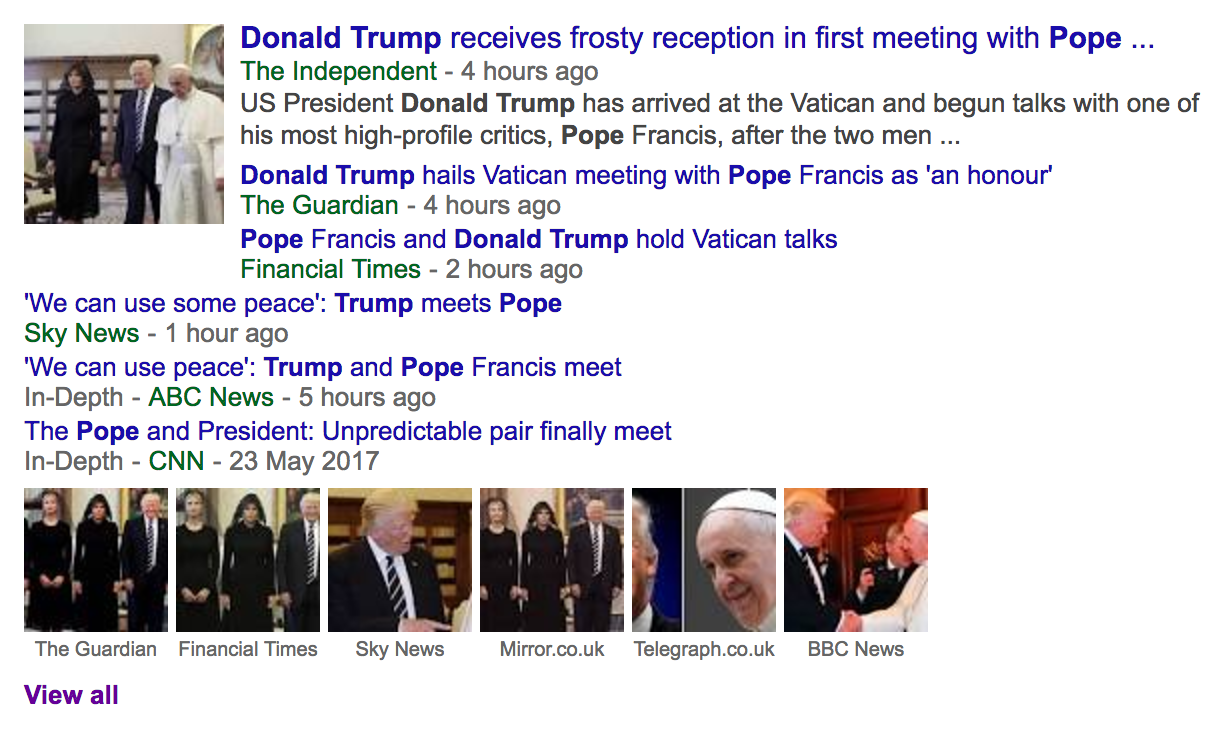
\includegraphics[width=\textwidth]{DonaldTrumpPope.png}
   \caption[A Google News Search on 24th May 2017]{A Google News search for stories about President Trump's visit to the Vatican on 24th May 2017.}
   \label{DonaldTrumpPope}
\end{figure}

When a consumer has to search for the news and find these sources themselves, it's more than probable that they will end up missing something. Also, which sources should they go to? And how many sources are enough to get a full and accurate picture? 

News Aggregators, such as Flipboard \cite{flipboard} and Apple News \cite{appleNews}, remove the requirement for a user to source articles themselves. The aggregators find the news and present it to the user in a way that is nicely grouped by topic. Other aggregators, such as Google News, allow consumers to search for news topics of their choosing as well, and present all the articles it finds on the same topic.

But these solutions don't go far enough, as they don't address a major issue - there is still a very high volume of news.

In July 2016, a study was conducted by the Statistic Brain Research Institute \cite{statisticBrain} that said that the average attention span of a person is now as low as 8.25 seconds \cite{attentionSpan}. In addition to this, the Institute's findings also said that the average person only reads 28\% of a webpage of average length (593 words). Another key finding was that users spend only 4.4 seconds to cover each additional 100 words on a webpage. It's simply not feasible for a consumer to go through several different sources' take on a piece of news, which is what many aggregators still expect them to do.

The primary objectives of my project are therefore two-fold. Firstly, the solution to the project needs to tackle the issue of users missing information because they need to find multiple sources for a topic. Secondly, the project will have to present a solution to the very high volume of news that a consumer needs to read. 

My solution is for a news aggregator that goes further than current products. NewSumm would have a primary aim of not only aggregating news, but of combining multiple sources' articles on a piece of news, and summarising them into one short piece. Using the example from before, the intention would be that the consumer only has to read one summary that incorporates the facts from several different sources on Trump's visit to the Vatican.

There is also the issue of reliability and trust to consider. The Digital News Report 2016 \cite{digitalNewsReport} found that in the United Kingdom only 50\% of readers trust what they see in the news. Could this be a case that there is simply so much news that it is hard to tell which is real? This could be the case because some readers will also be aware that a consequence of the new digital age is that anyone with an internet connection can create a blog and start spreading "fake news". 

\begin{figure}[h]
  \centering
    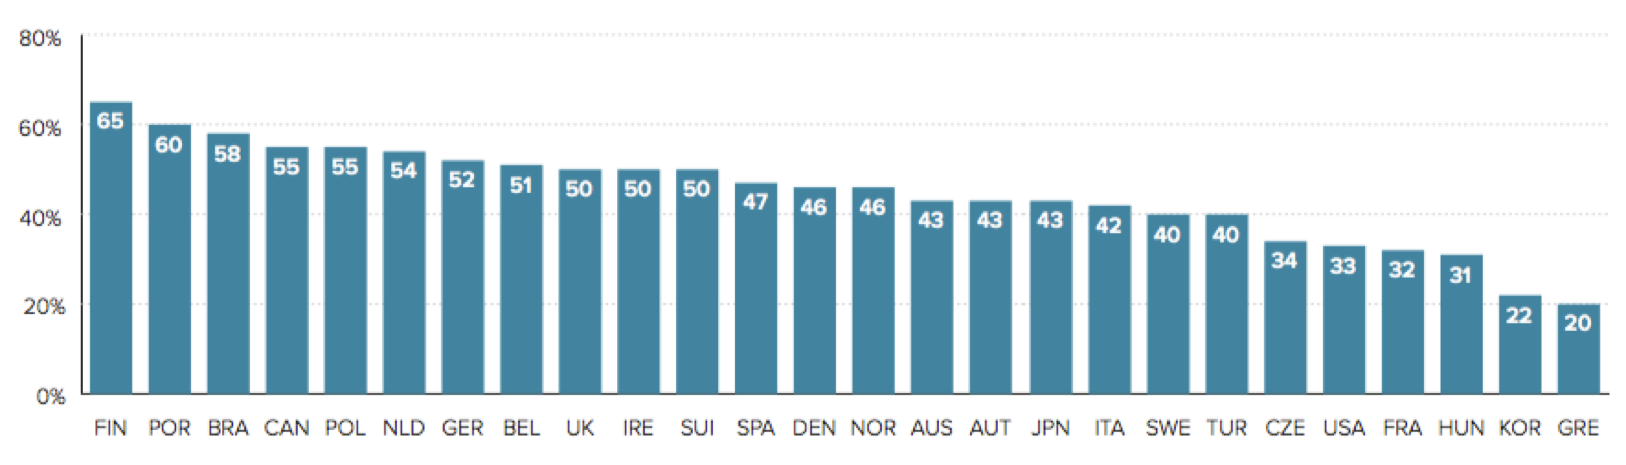
\includegraphics[width=\textwidth]{TrustInNews.png}
   \caption[The Digital News Report 2016 on trust in the news]{Digital News Report findings showed that when it came to trust in the news, in only a few countries was trust as high as 50\% in the accuracy of a piece of news. In countries such as the United States it is far lower.}
   \label{TrustInNews}
\end{figure}

Leading from this issue of trust, a secondary objective of the news aggregator would be that it produces content that users can be near certain is trustworthy and reliable - effectively a news aggregator that is free from "fake news".

Whilst it should be emphasised that the primary aim of NewSumm would be to reduce the sheer volume of news that a consumer has to read, it could be argued that the problem of "fake news" could be indirectly minimised in the same way that other news aggregators attempt to tackle the issue. This would be by limiting articles to trusted sources from across the political spectrum, by using only reputable news organisations and not considering articles from random blogs on the Internet. In addition to this, a clear indication when reading the summary of what facts different outlets all agree on, and what facts they either differ on or omit, will allow the user to easily corroborate parts of the story.

Beyond this, another objective of the project should be for the News Aggregator to allow users to eliminate elements of news, or sources themselves that they deem to be untrustworthy, thus alleviating consumer concerns about fake news.

A further secondary aim to this could be to allow a user to customise their summary, taking in information from the outlets of their choice (from the original "trusted" list). The advantage to this would potentially be that if a user decides that too many issues from one source are uncorroborated, they can remove them, and see only information from the other sources that have written about a topic. The disadvantage to this could be that if a user dismisses an entire section of the political spectrum as uncorroborated continuously, they'll pick up a political bias on the facts of the topic. Although, it could be said that the Digital News Report 2016 findings suggest that this is a feature that won't be used much. One of the more interesting findings in the report was that more than 60\% (in the United Kingdom) were concerned about the potential impact of personalising their news feeds. They felt that it could lead to both "missing information" and "missing challenging viewpoints".   

Using these aims and objectives as an indicator of future success, I then created NewSumm, as both a website and as an iOS application. The following sections set out NewSumm as an ambitious project that automatically fetches, labels, clusters and summarises articles without supervision. NewSumm was outlined as a user-friendly application that allows consumers a large level of control over what they read, through topic subscriptions and the ability to alter sources for summaries, as well as providing a daily digest for users who want them.

Whilst the ultimate goal of an abstractive summarisation tool in the back end proved to be infeasible, NewSumm, after thorough evaluation, was found to be an application that provides more than competent summarisation of articles and effective clustering that goes a large way to reducing the large volume of news that a consumer has to get through, thus satisfying the first primary aim. This was backed up by feedback from potential users through extensive surveys. Users spoke of the clean and slick design that NewSumm has, and were captivated by the concept of being able to "gather all sources on a particular topic at once", thus "saving time".

Going side by side with this evaluation of the fundamentals of the system itself was a rigorous analysis of the summaries produced to establish whether the system can be affected by the various political biases of its sources. The analysis exposed a potential vulnerability in the summariser, in that articles from sources that are considered to be purely factual can be marginalised, which in turn affects the success of the secondary aim of providing a near guarantee that all news produced is trustworthy. This is mitigated, however, by the theory presented earlier that by limiting the sources of news to trustworthy outlets the issue of "fake news" is largely solved.

%%%%%%%%%%%%%%%%%%%%%%%%%%%%%%%%%%%%%%%%%%%%%%%%%%%%%%%%%%%%%%%%%%%%%%%%%%%%%%%%%%%%%%%%%

\pagebreak

\section{Market Research}

\subsection{News Reading Habits}

\subsubsection{Digital News Report 2016}

\label{DigitalNewsReport}

Conducted by the Reuters Institute for the Study of Journalism \cite{reutersInstitute}\index{Reuters Institute for the Study of Journalism} in Oxford University \cite{oxford}\index{University of Oxford}, the Digital News Report\index{Digital News Report} \cite{digitalNewsReport} is an annual study that serves to investigate how people access and find out about news in various countries across the globe, including the United Kingdom\index{United Kingdom}.

The study attempts to cover, amongst other things how people get the news, how they use social media\index{Social Media}, what types of news they trust, and both the reasons to use and concerns about news aggregators. Findings of the report relevant to my concept are listed below:

\textbf{Reasons to use News Aggregators\index{News Aggregator!Reasons for use}}

\begin{figure}[h]
  \centering
    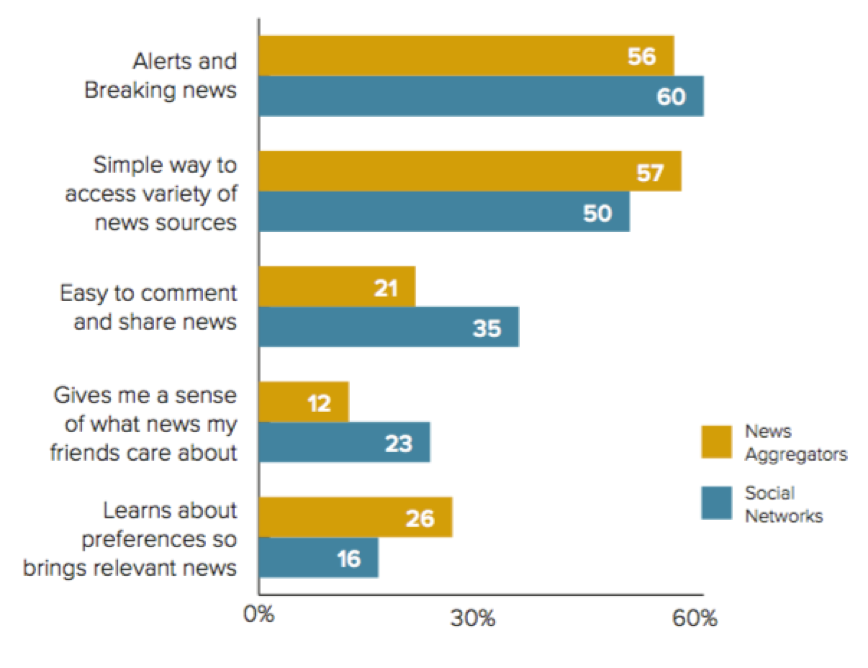
\includegraphics[scale=0.6]{WhySocialAggregatedNews.png}
   \caption[Why people use News Aggregators]{A graph showing why people use News Aggregators and Social Networks as news sources.}
   \label{WhySocialAggregatedNews}
\end{figure}

As shown in the graph in Figure \ref{WhySocialAggregatedNews} the key to the popularity of a News Aggregator is that it's simplicity and speed. It's important to bring news as soon as it happens, and it needs to provide access to a variety of different news sources. Of lesser importance is the social aspect - the need to comment and share the news, although the fact that 26\% of people want their preferences to influence the news that they're interested in should not be discounted.

\textbf{Concerns about Personalised News\index{News ! Personalised}}

\begin{figure}[h]
  \centering
    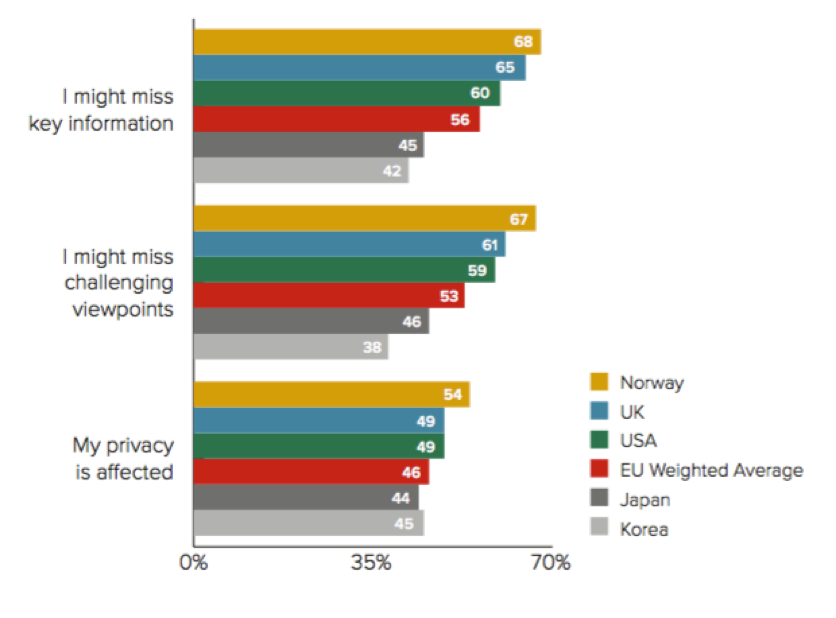
\includegraphics[scale=0.6]{PersonalisedNewsConcerns.png}
   \caption[Concerns with personalisation of News Feeds]{A graph showing the main three concerns that people have with Personalised News Feeds determining what they read.}
   \label{PersonalisedNewsConcerns}
\end{figure}

Key concerns, especially in the United Kingdom\index{United Kingdom}, with Personalised News\index{News ! Personalised} is that information might be incomplete. It is not difficult to see why this may be a concern - if you limit your news to a subset of the sources that might be available then it's possible to miss parts of the story - the parts that challenge aspects of the articles you're reading. It's therefore important that the project reflects this concern, which is why it is considered a secondary aim (see Section \ref{intro}). \\

\textbf{What should determine what someone reads next}

\begin{figure}[h]
  \centering
    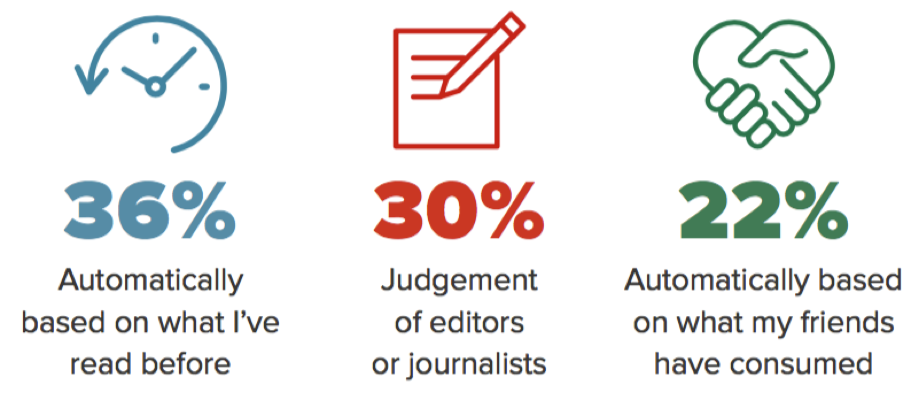
\includegraphics[scale=0.6]{HowPeopleTrustNews.png}
   \caption[What is a good way to get to the news?]{Key statistics in response to the question: Is this a good way to get the news?}
   \label{HowPeopleTrustNews}
\end{figure}

Least popular are algorithms that present news based on what people's friends have been reading. In general, according to the Reuters Institute \cite{reutersInstitute}\index{Reuters Institute for the Study of Journalism}, "People think *they* are the best judge of what's important to them." More interesting, is that people are now less inclined to allow journalists or editors to push articles to the top of reading lists than having an algorithm suggest similar stories to what they've just consumed. This could perhaps indicate that they aren't as trusting in journalists and editors as before - something that the Reuters Institute\index{Reuters Institute for the Study of Journalism} touches upon in an essay near the end of the report. \\

\textbf{Conclusions}

The Reuters Institute for the Study of Journalism\index{Reuters Institute for the Study of Journalism} is a trusted and respected organisation, and this study has been supported by institutions varying from media outlets such as the BBC \cite{bbc}\index{BBC}, news search engines such as Google\index{Google}\index{Google!Search Engine}, and other Universities, such as University of Canberra \cite{canberra}\index{University of Canberra}. Importantly, it's also supported by regulators, including Ofcom \cite{ofcom}\index{Ofcom}, which is the regulator in the United Kingdom\index{United Kingdom}. 

The survey was conducted on their behalf by YouGov \cite{yougov}\index{YouGov}, which is a highly respected polling company in the United Kingdom\index{United Kingdom}, and it surveyed more than 50,000 people, including over 2000 in the United Kingdom. In addition, the report is coupled with numerous essays on various key points that arose from the study. The writers of these essays varied from the Director of Research at the Reuters Institute\index{Reuters Institute for the Study of Journalism} to the Chief Executive Officer of The New York Times \cite{newYorkTimes}\index{New York Times}.

As a result of this, I deemed the Digital News Report 2016\index{Digital News Report} \cite{digitalNewsReport} to be a very reliable source of information with regards to how people read the news, and their preferences in the field. 

\subsubsection{Potential User Survey\index{User!Survey}}

\label{survey}

Following this initial research I decided to conduct a survey of potential users to delve into more specific aspects of News Reading Habits. I was more focused on the number of sources people use to ascertain the facts about a piece of news. I also asked questions regarding the summarisation\index{Summarisation} of news and news digests.

I was interested in the questions about summarisation and digests after reading some data from a study conducted by the Statistic Brain Research Institute \cite{statisticBrain}\index{Statistic Brain Research Institute}. Statistic Brain conducted a study in July 2016 that suggested that the average attention span of a human is now only 8.25 seconds \cite{attentionSpan}. They coupled the presentation of this data with statistics about people browsing the internet taken from the paper \emph{Not Quite the Average:
An Empirical Study of Web Use}\index{Not Quite the Average: An Empirical Study of Web Use} \cite{empiricalStudyofWebUse}. The statistics suggest that the average user only reads 28\% of the words on the average webpage, and that for each additional 100 words beyond that, the user would only spend an additional 4.4 seconds on the page.

Admittedly, the paper was written in 2008, and so might not reflect average web browsing activity, but it raised a question worth answering in my opinion. Do users actually read full articles on the news, and if not, would summarising articles help make sure they didn't miss out on key points, thus counteracting an issue discovered in the Digital News Report 2016\index{Digital News Report} \cite{digitalNewsReport} (Section \ref{DigitalNewsReport})? 

The survey was presented on Google Forms \cite{googleForms}\index{Google!Forms} and was answered by 96 respondents. A link to the original survey can be found in Appendix \ref{nrh}. Further findings are shown below:

\begin{enumerate}

\item \textbf{How often do you read the news?}

\begin{figure}[ht!]
  \centering
    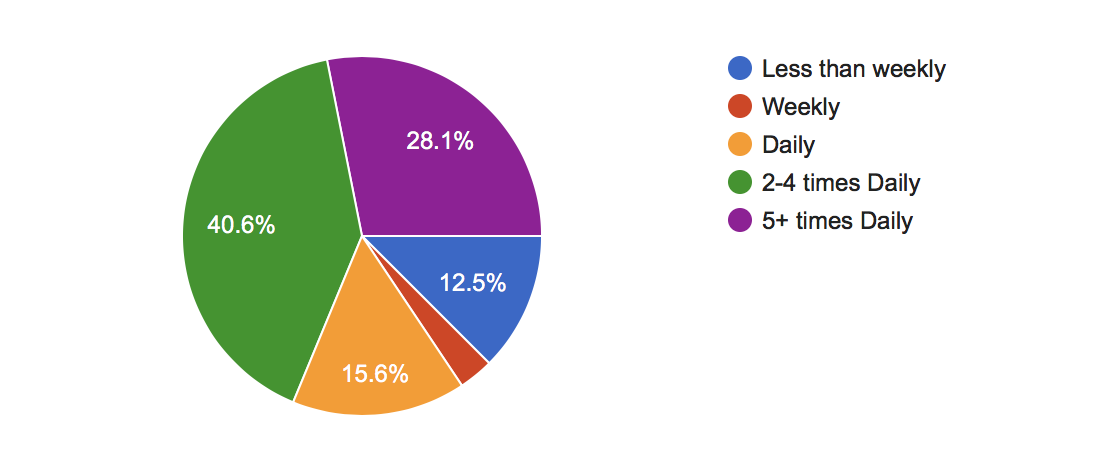
\includegraphics[scale=0.7]{01HowOftenDoYouReadTheNews}
   \caption[Survey Graph surrounding how often news is read]{A pie chart showing how often people read the news.}
   \label{SurveyHowOftenDoYouReadTheNews}
\end{figure}

The first question (Figure \ref{SurveyHowOftenDoYouReadTheNews}) on the survey was designed to ascertain how often people read the news. Overall, well over 80\% of respondents said that they read the news at least daily, and nearly 60\% more than once per day. \\

\item \textbf{How many sources do you read?}

\begin{figure}[ht!]
  \centering
    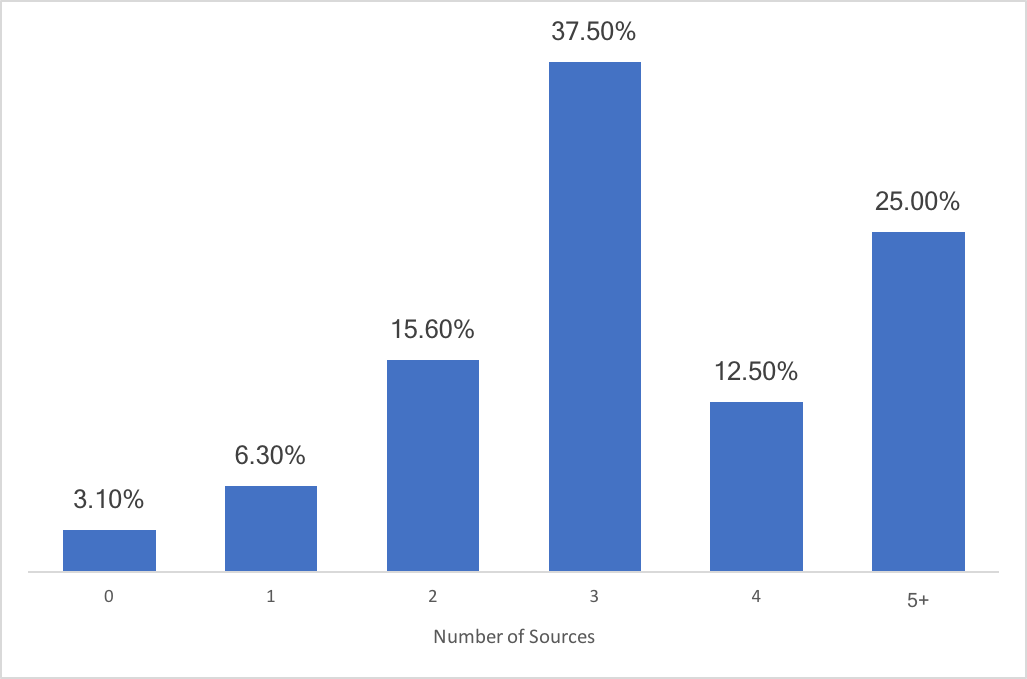
\includegraphics[scale=0.7]{02HowManySourcesDoYouRead}
   \caption[Survey Graph asking how many sources are used]{A bar graph showing how many sources people normally use for a source of news.}
   \label{SurveySources}
\end{figure}

Next I asked about how many sources a user read. It was quite rare for someone to use only one source for a piece of news. In fact, over 90\% said that they used two or more sources, with three and five sources being the most prominent selections. \\

\item \textbf{Are these the same sources every time?}

\begin{figure}[ht!]
  \centering
    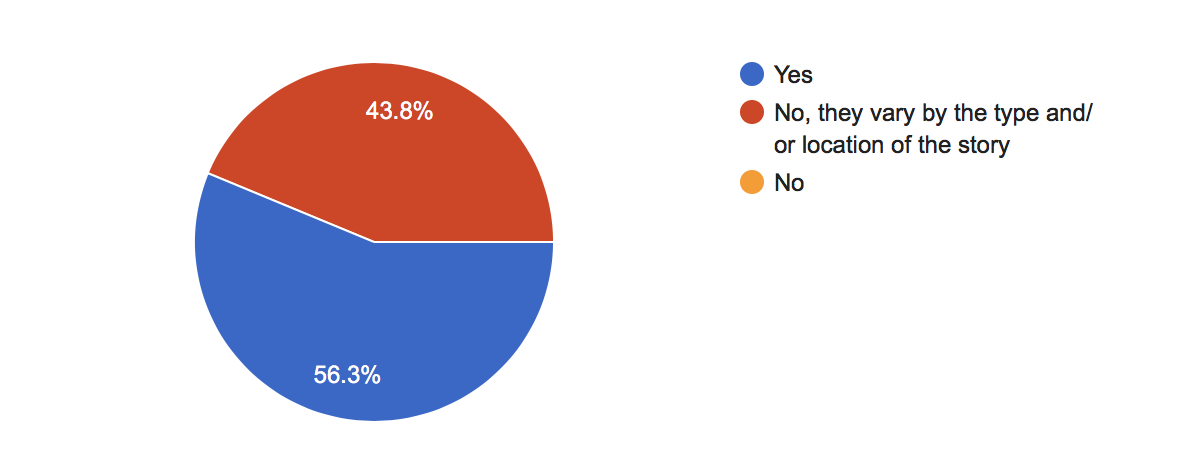
\includegraphics[scale=0.7]{03AreTheseTheSameSourcesEverytime}
   \caption[Survey Graph about consistency of sources]{A pie chart showing whether people use the same sources every time.}
   \label{SurveySourceConsistency}
\end{figure}

The respondents were a lot more split on the question of consistency of sources, although more than half said that they used the same sources every time, with 43.8\% saying that they vary their sources based on the type and/or location of the news story. \\

\item \textbf{How much of an article do you normally read?}

\begin{figure}[ht!]
  \centering
    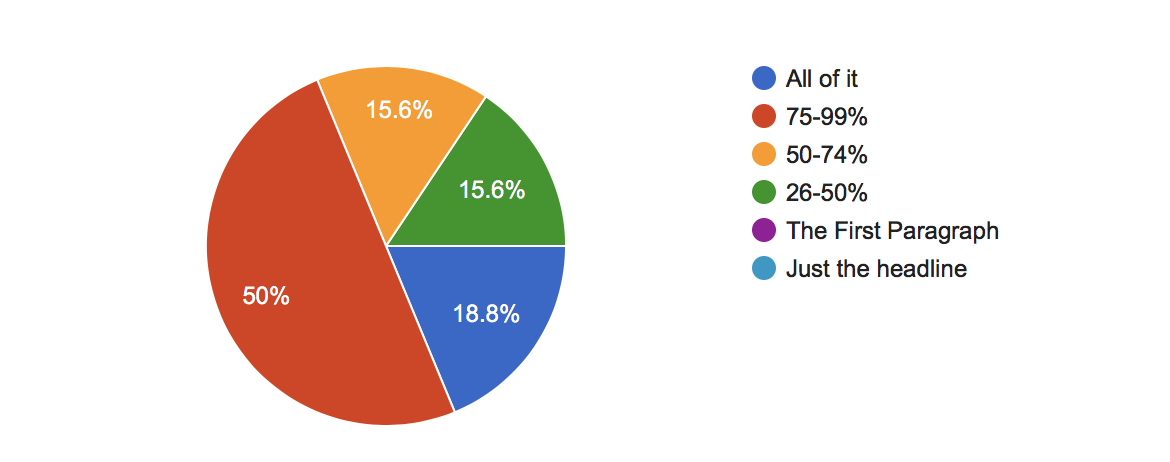
\includegraphics[scale=0.7]{05HowMuchOfAnArticleDoYouRead.png}
   \caption[Survey Graph regarding how much of an article is read]{A pie chart showing how much of articles people normally read.}
   \label{SurveyArticleLength}
\end{figure}

I further expanded upon the initial reading I had done about attention spans by asking potential users how much of articles they normally read. Only 18.8\% of respondents said that they read the entirety of articles (Figure \ref{SurveyArticleLength}), and as much as 15.6\% confess that they read less than 50\% of an article on average. It's plausible that the users could be missing key facts through not reading the entire article. On reflection, I could have also asked if this was a concern to those users. \\

\item \textbf{If an article was presented as a shorter summary, would you read more/all of it?}

\begin{figure}[ht!]
  \centering
    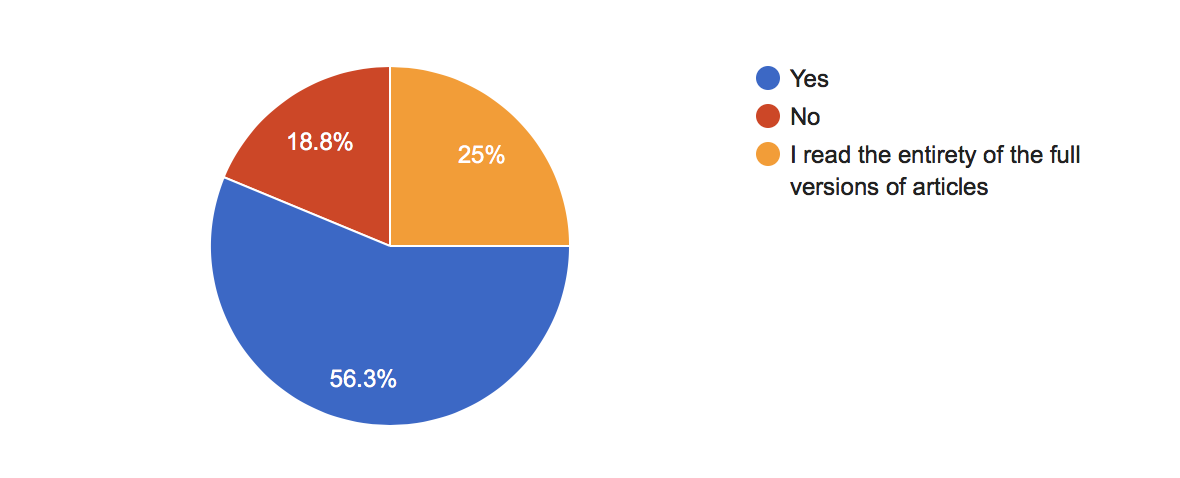
\includegraphics[scale=0.7]{06WouldYouReadAShorterSummary.png}
   \caption[Survey Graph regarding summarisations of articles]{A pie chart showing what percentage of people would read a shorter summary of an article.}
   \label{SurveyArticleLength}
\end{figure}

Another question asked was whether reading a shorter summary would result in users reading more or all of the article. Encouragingly, more than half (56.3\%) of respondents said that they would read a shorter summary. \\

\item \textbf{Would you read a summary of different articles on the same topic combined?}

\begin{figure}[ht!]
  \centering
    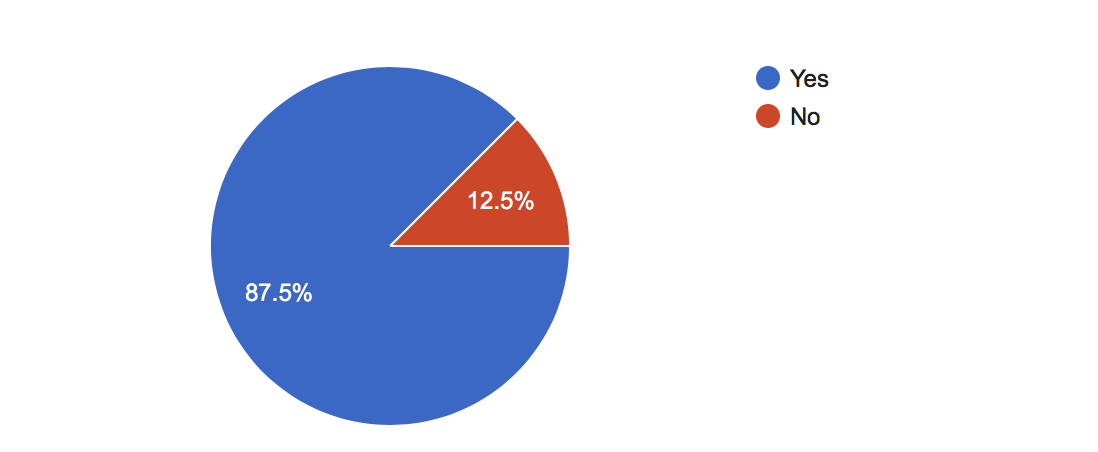
\includegraphics[scale=0.7]{07WouldYouReadASummaryOfArticlesCombined}
   \caption[Survey Graph about combining articles]{A pie chart showing whether people would read a summary of different articles on the same topic combined.}
   \label{SurveySummarisedArticles}
\end{figure}

With this question (Figure \ref{SurveySummarisedArticles}) I aimed to obtain an idea from potential users as to whether combining articles about the same topic from different sources and then summarising it would be considered useful. The question got a resounding response, with as much as 87.5\% saying that they would read a summary like this.  \\

\item \textbf{Would you use a News Aggregator that summarised articles?}

\begin{figure}[ht!]
  \centering
    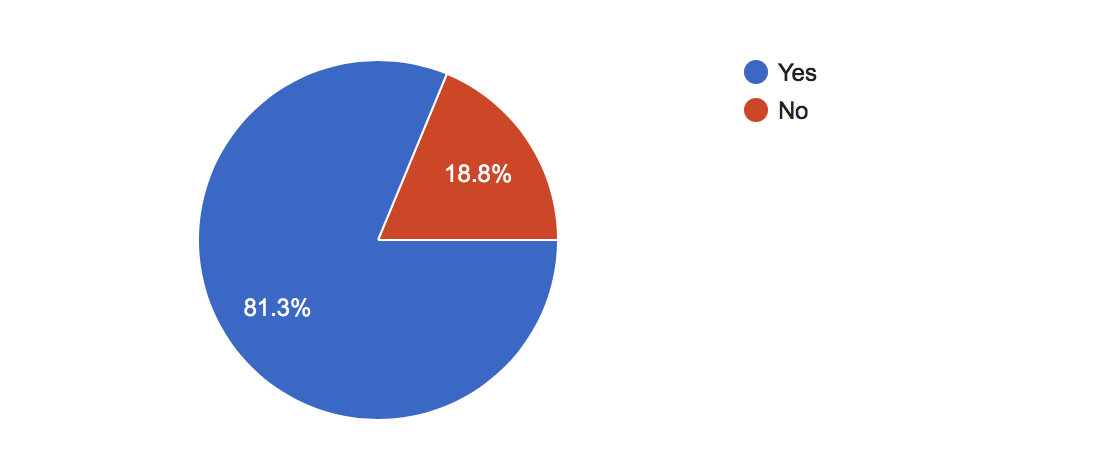
\includegraphics[scale=0.7]{08WouldYouUseANewsAggregatorThatSummarised}
   \caption[Survey Graph concerning News Aggregators and summarisation]{A pie chart showing answers to the question: "Would you use a News Aggregator\index{News Aggregator} that summarised articles".}
  \label{NewsAggregatorThatSummarised}
\end{figure}

Consolidating the findings of the previous question was the fact that 81.3\% said they would use a News Aggregator\index{News Aggregator} that summarised\index{Summarised} articles (Figure \ref{NewsAggregatorThatSummarised}). Amongst those who said they wouldn't, there were comments along the lines of "I'm not great with technology" given as explanation. An interesting comment however, said that "nuance could be lost in the summarisation". This is a valid point, and so a key point of the evaluation\index{Evaluation} process will have to be focused on the summarisation of articles itself, to ensure it's not losing important information at any stage.\\

\item \textbf{How often do you search for news on a specific topic?}

\begin{figure}[ht!]
  \centering
    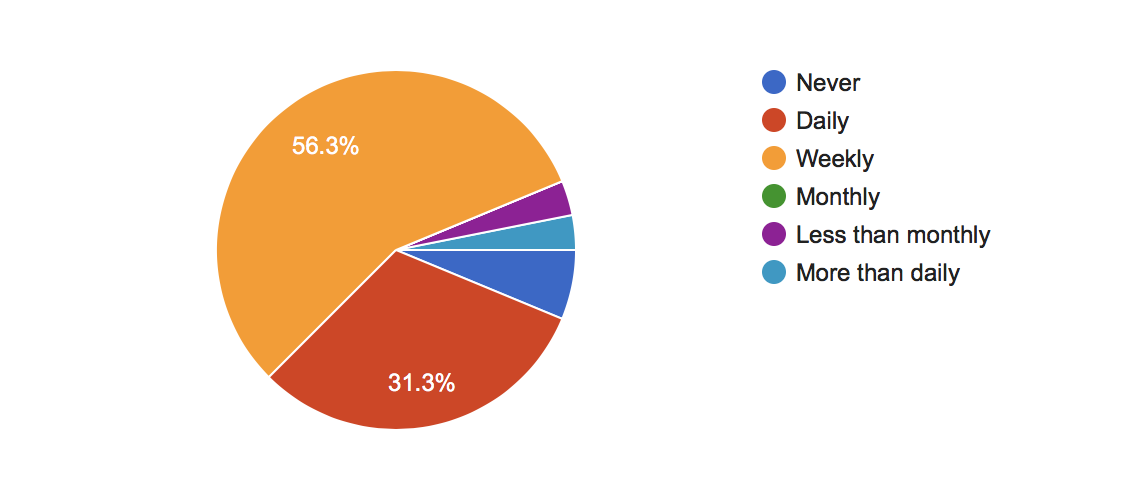
\includegraphics[scale=0.7]{10HowOftenDoYouSearchForASpecificTopic}
   \caption[Survey Graph regarding searching for topics in the news]{A pie chart showing how frequently people search for news on a specific topic.}
   \label{SurveySearchingForTopics}
\end{figure}

For the questions in Figure \ref{SurveySearchingForTopics} I tried to get an idea of how much people search for news on a specific subject of interest to them. In general, this came out to be less frequent then reading the news itself, with just over half the respondents saying that they search for a specific topic weekly. However, a healthy proportion (31.3\%) search daily for specific topics, and some search even more often than this.\\

\item \textbf{Should the news aggregator have the ability to search for a specific topic?}

\begin{figure}[ht!]
  \centering
    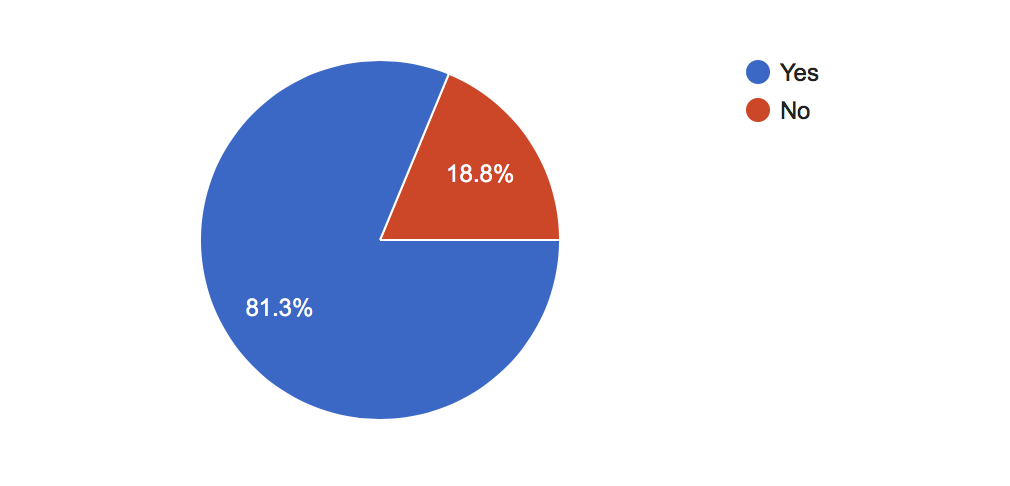
\includegraphics[scale=0.7]{11ShouldNewsAggregatorProvideSearchingForSpecificTopic.png}
   \caption[Survey Graph regarding news aggregators and searching]{The answers to a question asking if the News Aggregator should have the ability to search for a specific topic.}
\end{figure}

As much as 81.3\% of respondents agreed that the News Aggregator\index{News Aggregator} should have a function to search for specific topics. \\

\item \textbf{Do you like services such as news digests that prepare lists of articles each day that apply to a topic you may be interested in?}

\begin{figure}[ht!]
  \centering
    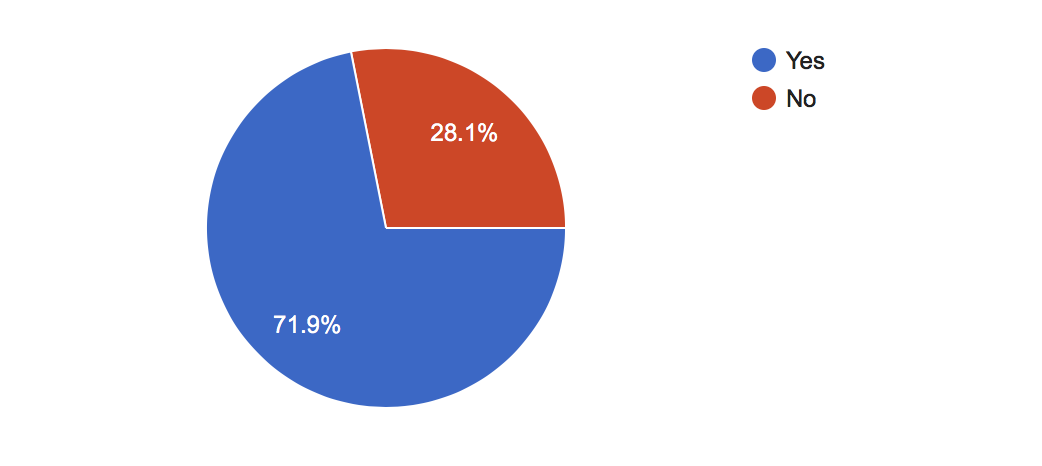
\includegraphics[scale=0.7]{12DoYouLikeServicesThatProduceDigests}
   \caption[Survey Graph about News Digests]{A pie chart showing people's attitudes towards News Digests.}
   \label{SurveyDigests}
\end{figure}

The next question, shown in Figure \ref{SurveyDigests} centred around News Digests\index{News Digests}. Nearly 72\% of respondents said that they liked services that provide news digests.\\

\item \textbf{How often should these news digests be updated?}

\begin{figure}[ht!]
  \centering
    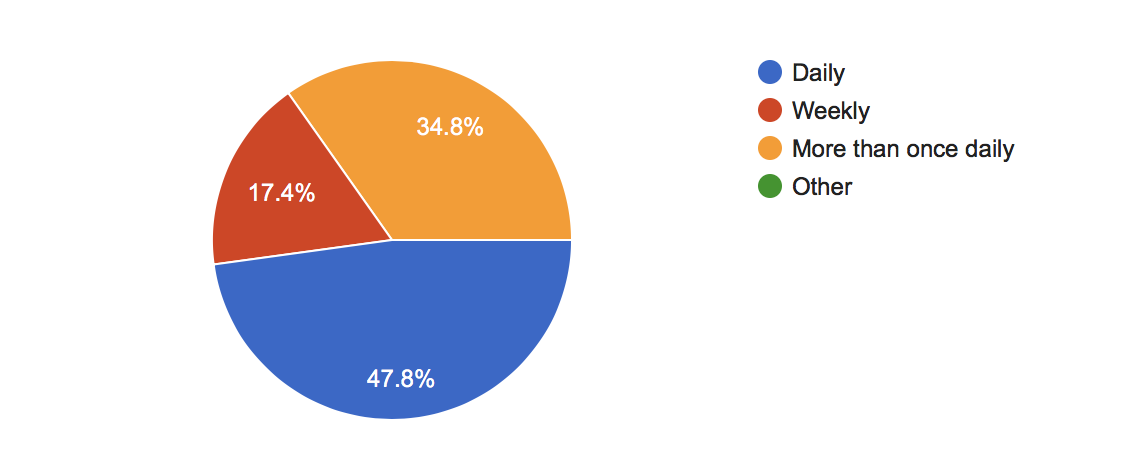
\includegraphics[scale=0.7]{13HowOftenShouldTheseDigestsBeProduced}
   \caption[Survey Graph about News Digests' frequency]{Responses regarding how frequently news digests should be updated.}
\end{figure}

People who were in favour of news digests in general felt that these should be updated at least daily (47.8\%), with a further 34.8\% on top of that saying it should be updated more than once.\\

\item \textbf{What platform should the aggregator be developed for?}

\begin{figure}[ht!]
  \centering
    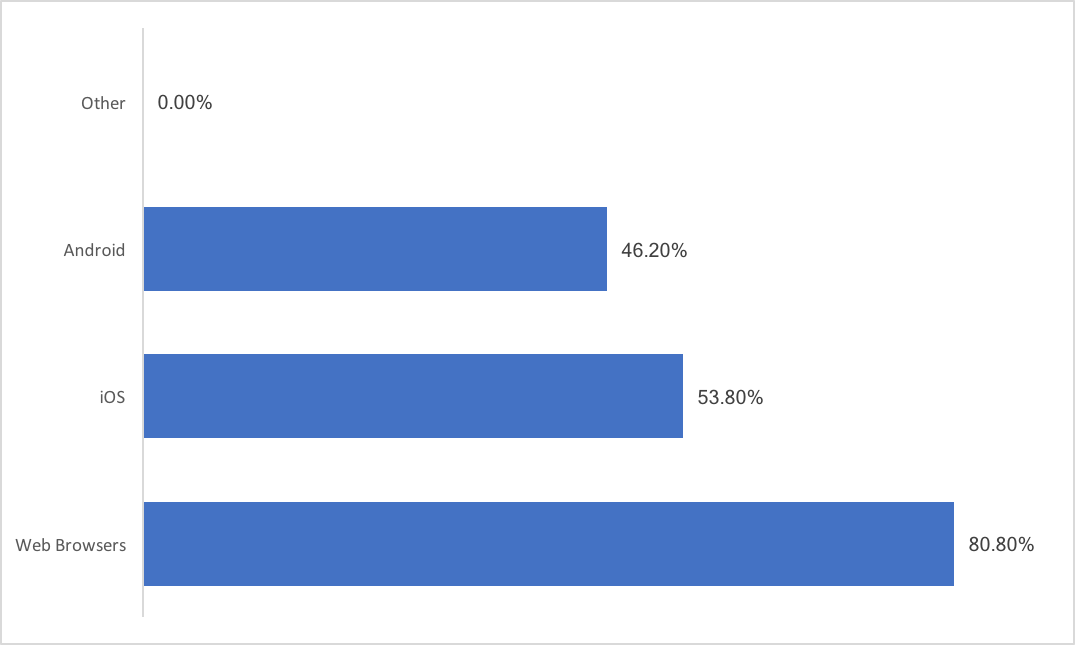
\includegraphics[scale=0.7]{09WhatPlatform.png}
   \caption[Survey Graph concerning potential platforms]{A bar chart showing responses when asked which platform they'd rather see the news aggregator developed for.}
   \label{Survey Platform}
\end{figure}

Finally, respondents were asked which platform they would prefer to see the news aggregator developed for. 80.8\% said they'd want a version for web browsers, and 53.8\% for iOS and 46/2\% for Android. This would suggest that I should develop a web solution and then move to a mobile platform afterwards if there is time.\\

\end{enumerate}
 
\subsection{Related Products}

\subsubsection{Google News}\index{Google!News}

\begin{figure}[H]
  \centering
  \begin{subfigure}{0.8\textwidth}
        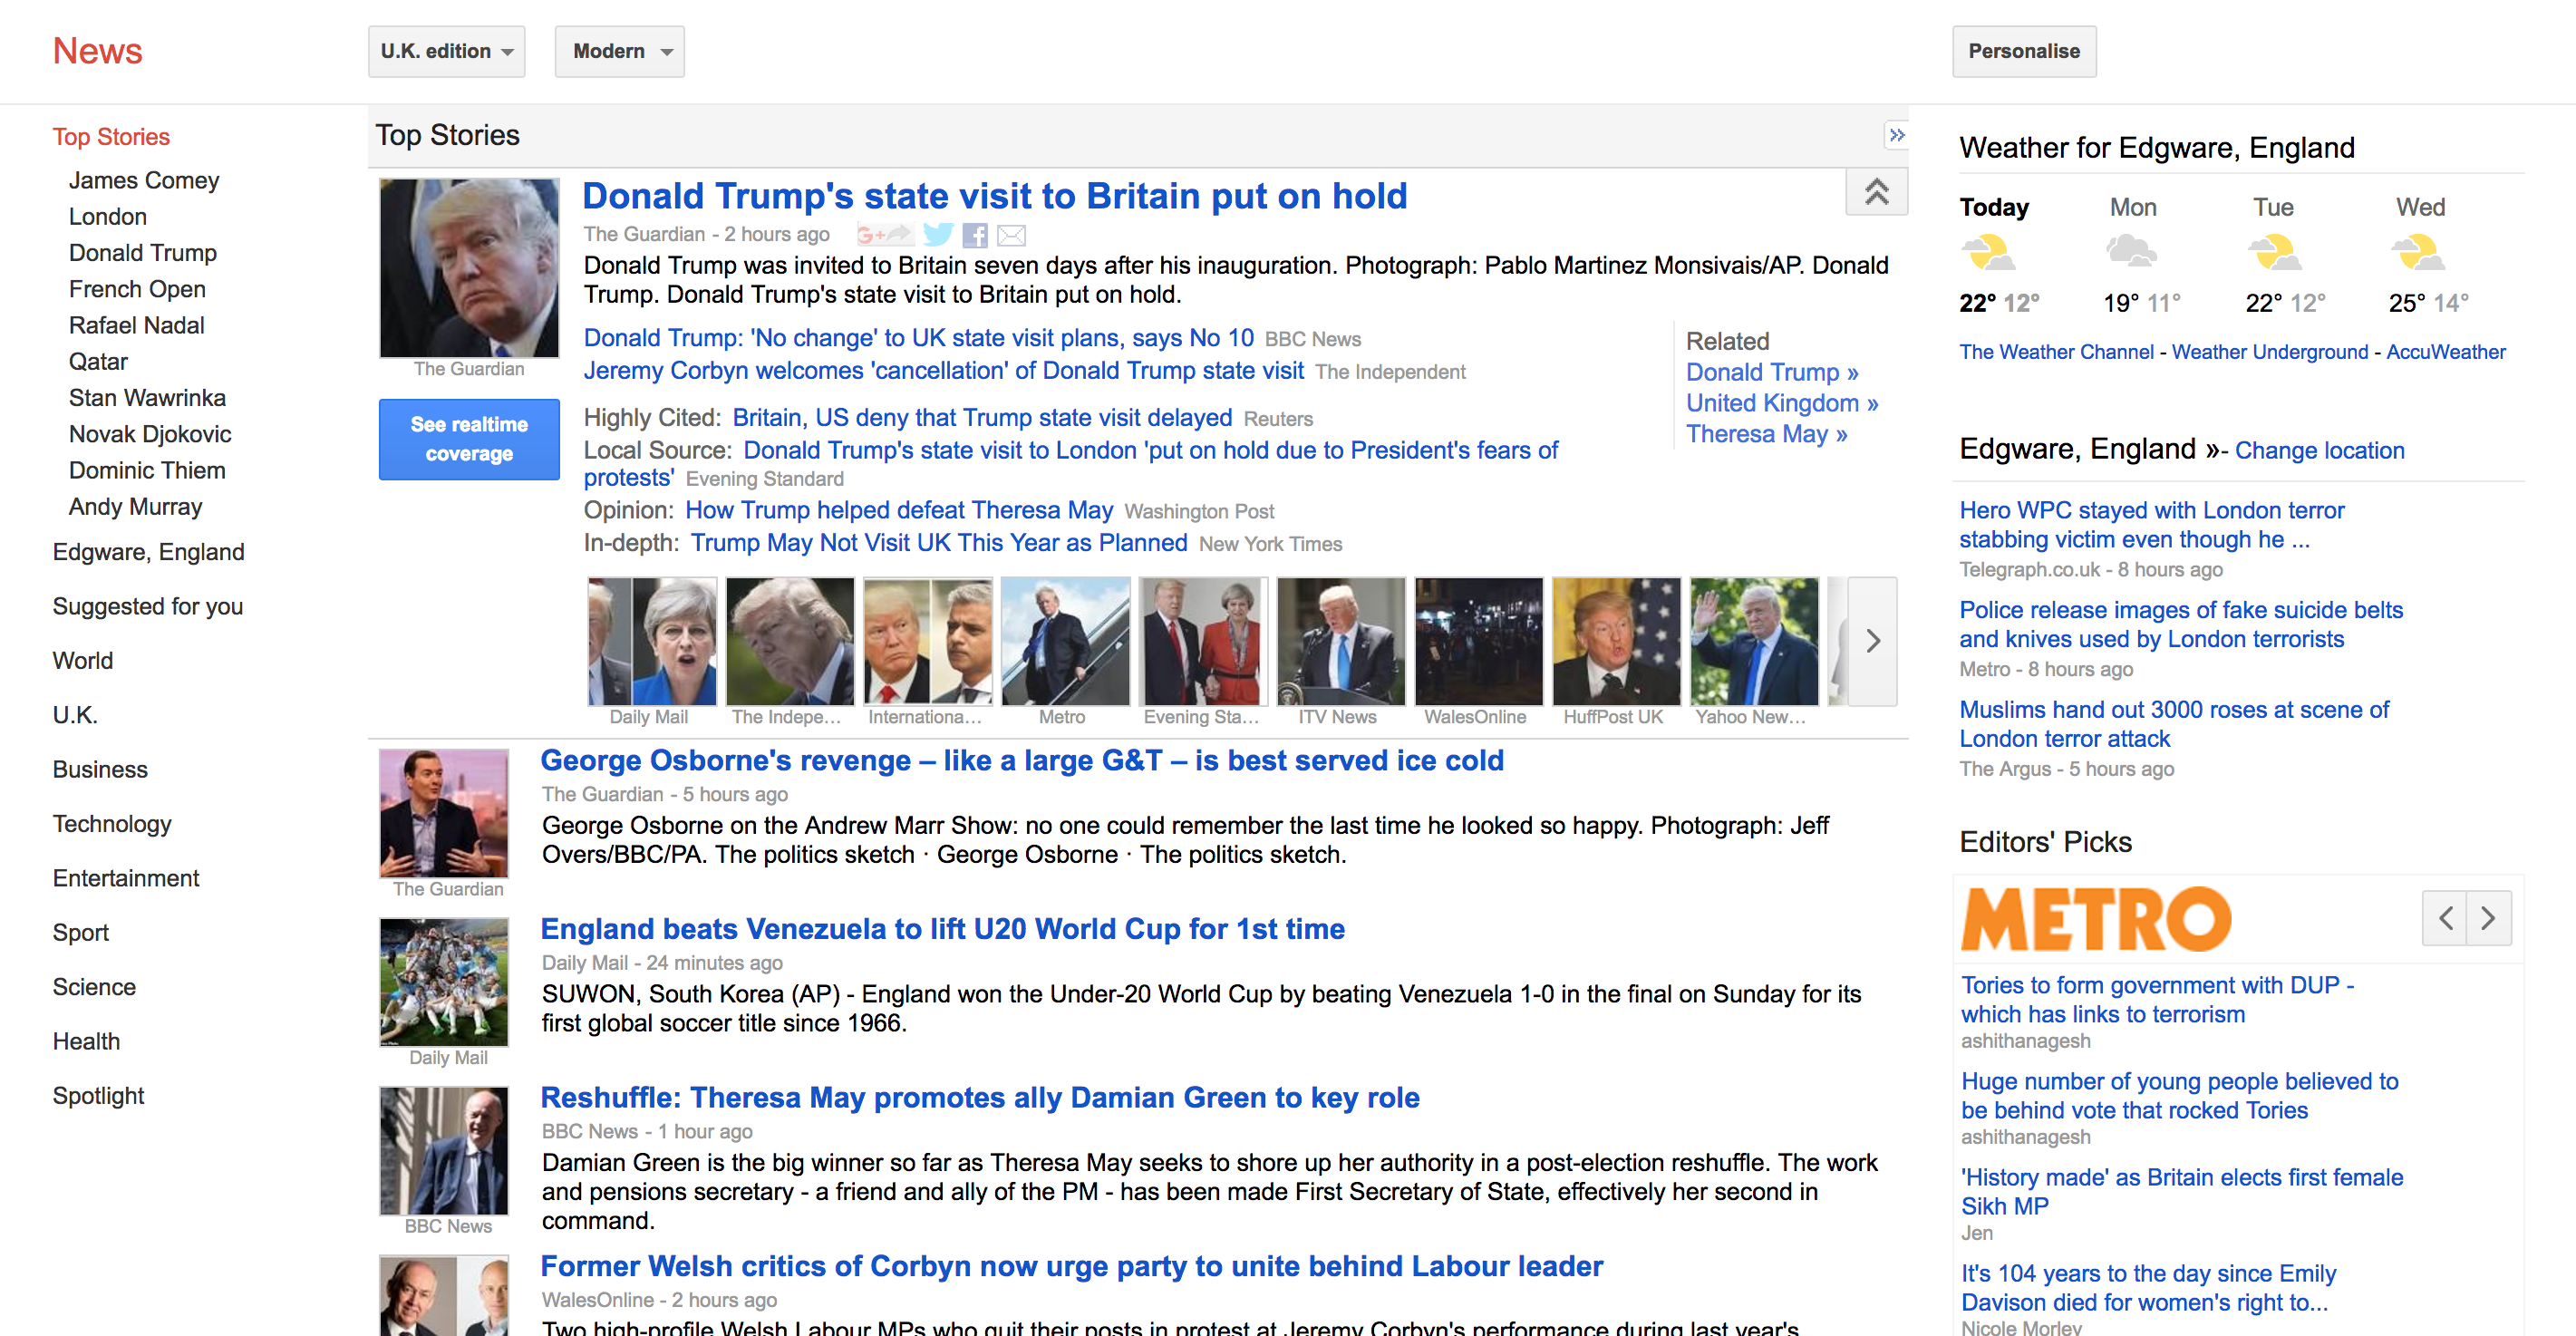
\includegraphics[width=\textwidth]{GoogleHome}
        \caption[Screenshot from the Google News home page]{A Section of the homepage for Google News \cite{googleNews}.}
        \label{GoogleNewsHome}
    \end{subfigure}
    
    \begin{subfigure}{\textwidth}
    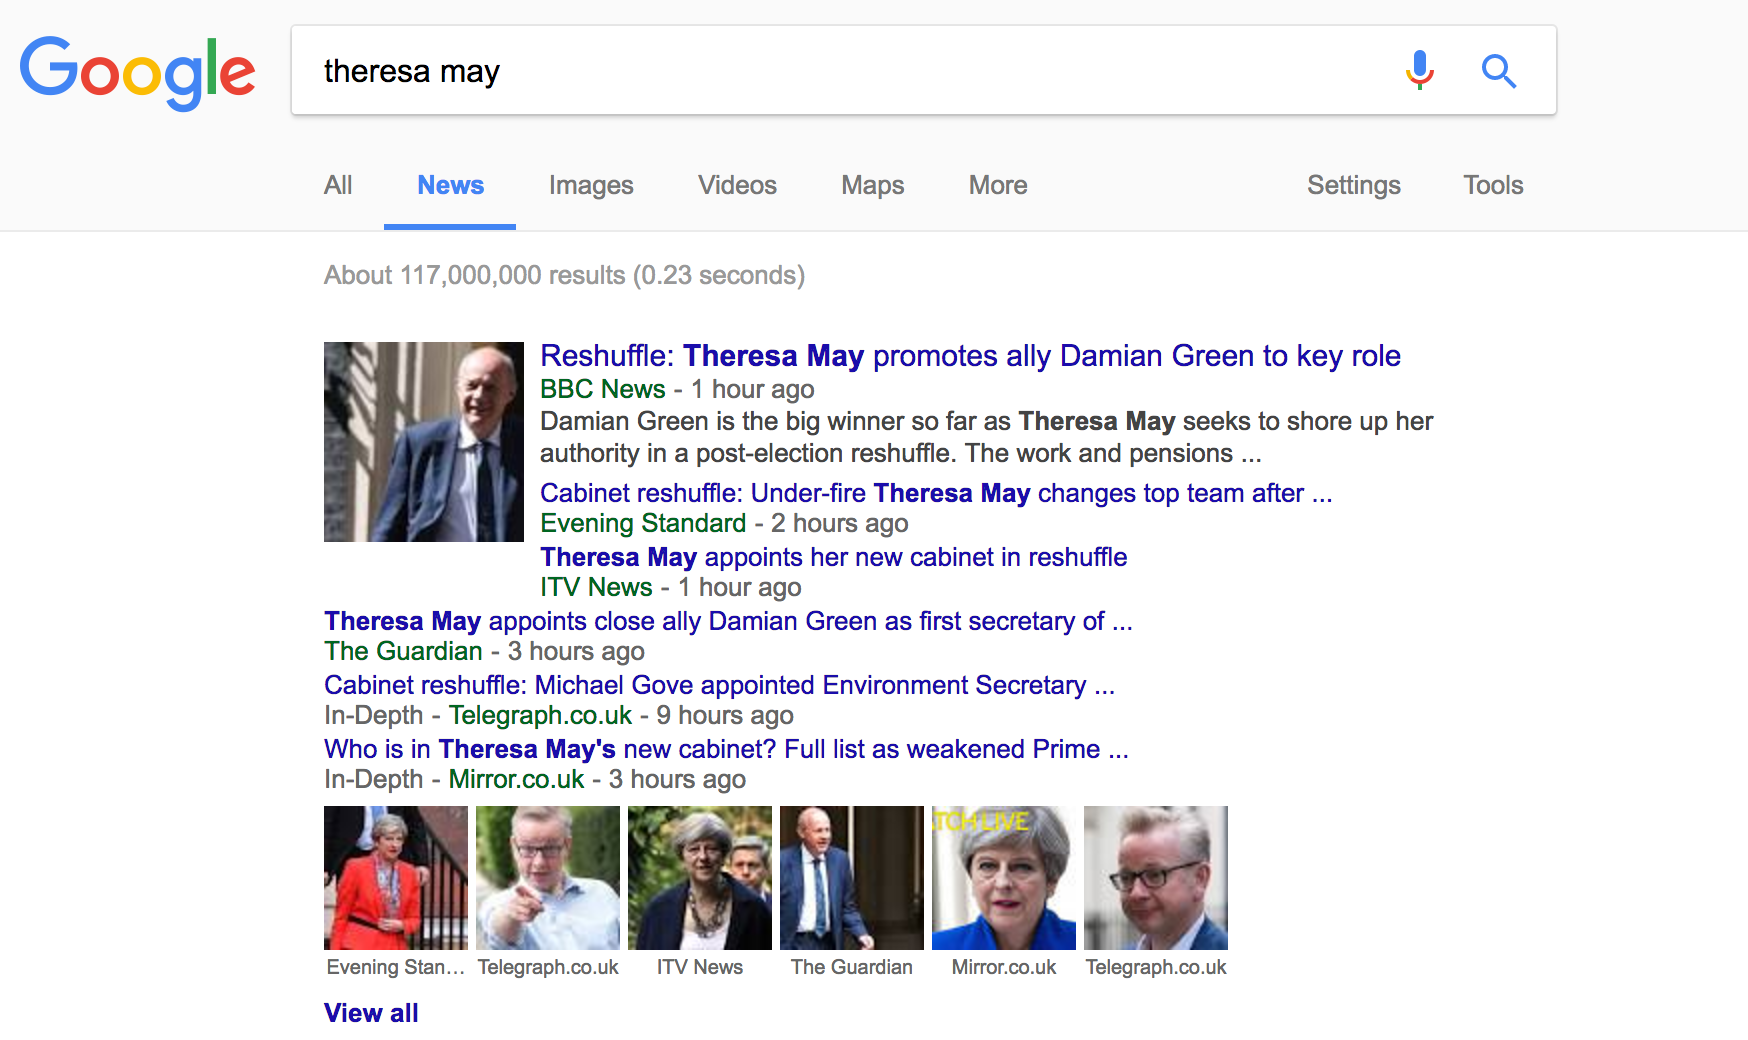
\includegraphics[width=\textwidth]{GoogleUber}
   \caption[Screenshots from a Google News search]{Google News uses clustering techniques to group articles about the same topic together. }
   \label{GoogleNewsUber}
   \end{subfigure}
   \caption[Screenshots from Google News]{Screenshots from Google News.}
\end{figure}

Initially developed early in the century and released in 2006, Google News \cite{googleNews} is a free-to-use news aggregator. Google News operates in a similar manner to the traditional Google \cite{google} search engine, thus making it a go to aggregator when searching for a specific topic. Google News also groups "similar" articles together using Clustering\index{Clustering} techniques \cite{googleClustering}. Google News operates purely as a go-between - when clicking on an article the user is taken straight to the media source itself, rather than being able to read the article on Google News itself. 

\subsubsection{Flipboard}\index{Flipboard}

\begin{figure}[H]
  \centering
  \begin{subfigure}[t]{0.3\textwidth}
        
\includegraphics[width=\textwidth]{FlipboardHome.PNG}
        \caption{Users can subscribe to "magazines" that they may be interested in.}
        \label{FlipboardHome}
    \end{subfigure}
    \qquad
    \begin{subfigure}[t]{0.3\textwidth}
    
\includegraphics[width=\textwidth]{Flipboard.PNG}
   \caption{All users are subscribed to \emph{Cover Stories}, which puts together the latest most popular news.}
   \label{FlipboardDailyEdition}
   \end{subfigure}
   \caption[Screenshots from the Flipboard app]{Screenshots from the Flipboard app.}
\end{figure}

Flipboard \cite{flipboard} is a much more recent attempt at a news aggregator (developed in 2010), and relies on the concept of users subscribing to "magazines" on different topics. There's a central "cover page" on the home page that shows the most recent stories from across all a user's subscriptions. Like Google News\index{Google!News}, links from the desktop website send the user to the original media source, while links from within the mobile applications open a browser within the app itself.

\subsubsection{Yahoo News Digest}\index{Yahoo News Digest}

\begin{figure}[ht!]
  \centering
  \begin{subfigure}[t]{0.3\textwidth}
        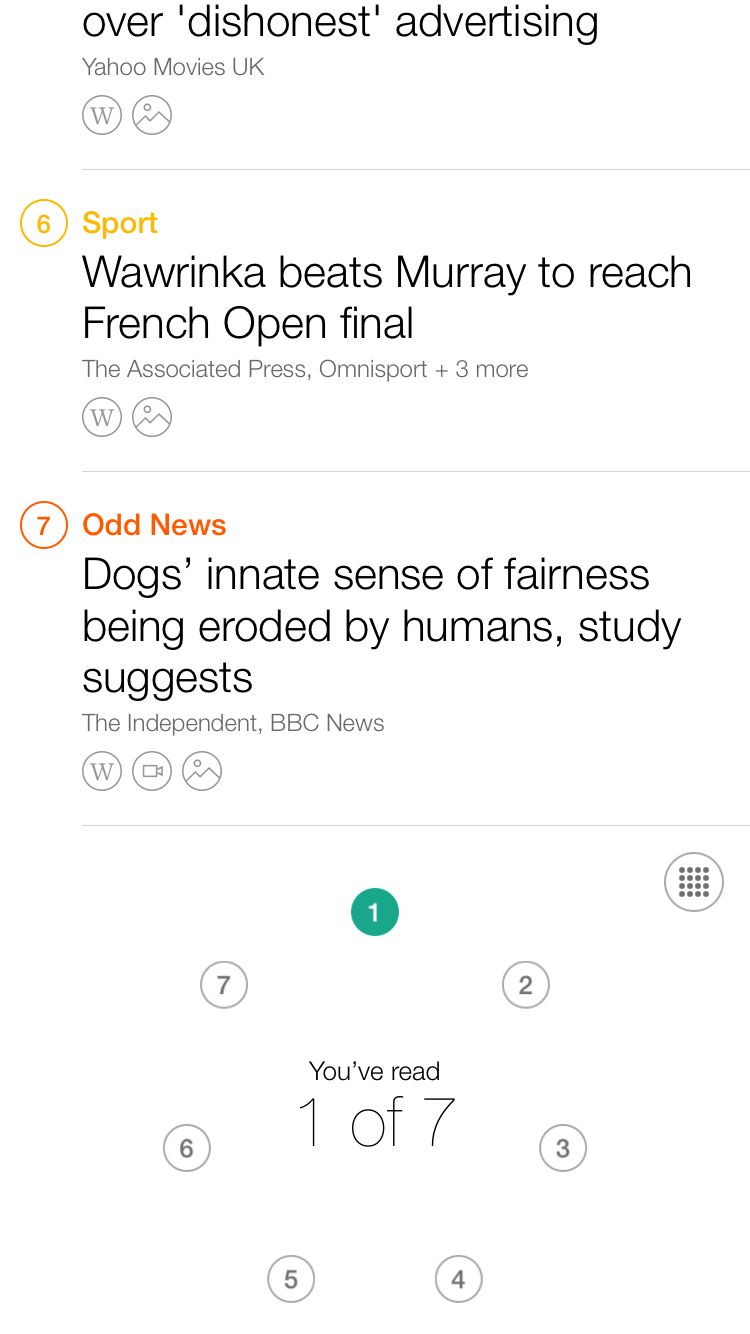
\includegraphics[width=\textwidth]{YNDHome.PNG}
        \caption{A Section of the home screen, which displays the top ten stories for the day.}
        \label{YNDHome}
    \end{subfigure}
    \qquad
    \begin{subfigure}[t]{0.3\textwidth}
    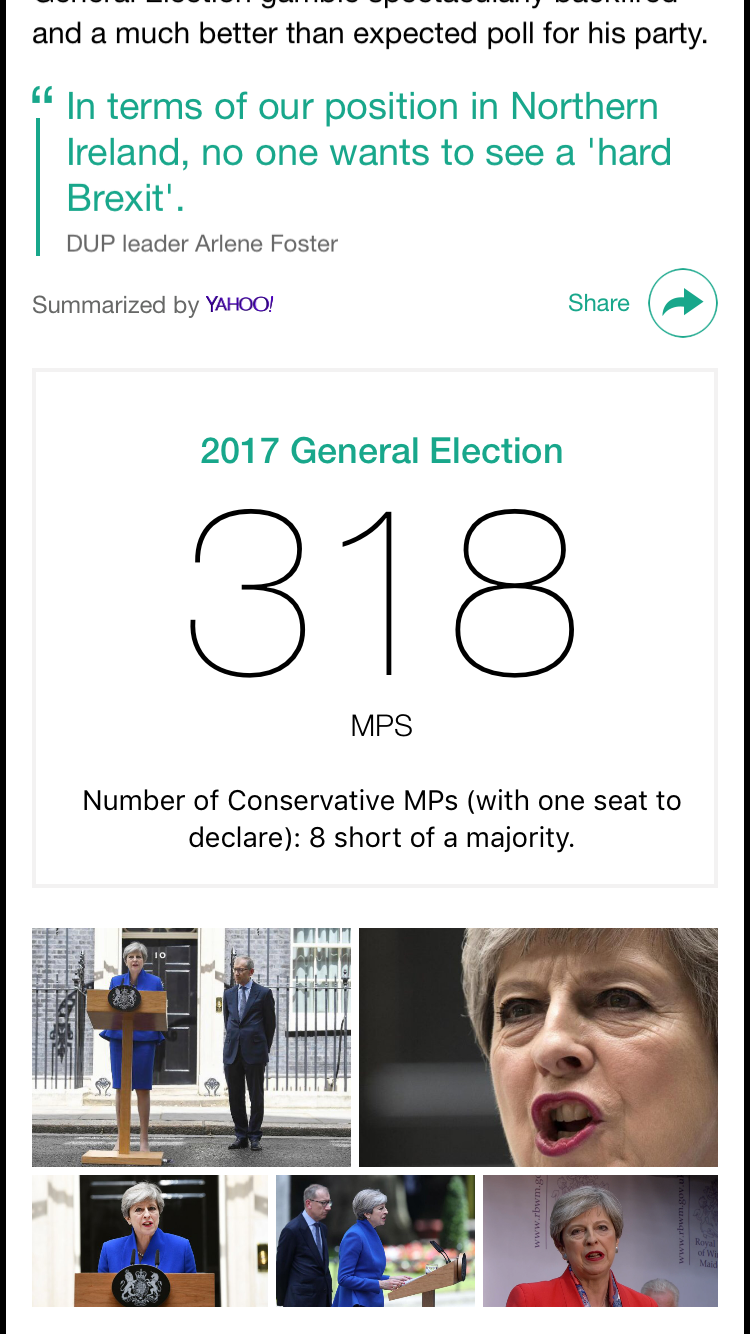
\includegraphics[width=\textwidth]{YNDInfo.PNG}
   \caption{The Yahoo News Digest app provides links and infographics that are relevant to the article.}
   \label{YNDInfo}
   \end{subfigure}
   \caption[Screenshots from the Yahoo News Digest app]{Screenshots from the Yahoo News Digest app \cite{yahooNewsDigest}.}
\end{figure}

Yahoo News Digest \cite{yahooNewsDigest} is a direct evolution from Summly \cite{summly}, which was an app that summarised news. Yahoo News Digest is a phone application that creates two digests a day: one in the morning and one in the evening. Each digest contains the ten leading articles from the previous 12 hours. Each article provides a summary of the story and links to relevant other pages - such as articles from Wikipedia \cite{wikipedia}.

\subsubsection{Apple News}\index{Apple!News}

\begin{figure}[ht!]
  \centering
  \begin{subfigure}[t]{0.3\textwidth}
        
\includegraphics[width=\textwidth]{AppleHome.PNG}
        \caption{The home screen for the Apple News app.}
        \label{AppleHome}
    \end{subfigure}
    \qquad
    \begin{subfigure}[t]{0.3\textwidth}
    
\includegraphics[width=\textwidth]{AppleSources.PNG}
   \caption{Apple News allows users to select sources and topics to be their favourites.}
   \label{AppleSources}
   \end{subfigure}
   \caption[Screenshots from the Apple News app]{Screenshots from the Apple News app \cite{appleNews}.}
\end{figure}

Apple News \cite{appleNews} is an application that is installed by default on all recent iOS devices. Apple's default attempt at a news aggregator allows users to select their preferred news sources, and from a selection of topics. Apple \cite{apple} then presents on a home screen news from those sources and topics. Clicking on each article keeps it in the native application, rather than sending the user to the media source itself.

\subsubsection{Comparing the existing products}

The existing products are compared in Table \ref{relatedProductsTable} on page \pageref{relatedProductsTable}.

\begin{sidewaystable}
    \begin{tabular}{p{2.5cm}|p{8.75cm}|p{8.75cm}}
    \textbf{Product} & \textbf{What it does well} & \textbf{What it doesn't do well} \\ \hline
    Google News & \tabitem Groups similar articles together & \tabitem Doesn\'t host articles itself - therefore making it harder to navigate than perhaps could be possible. Although, this could be to avoid any copyright issues. \\ & \tabitem Similar to a traditional search engine and so is easy to use\\ & \tabitem Obtains articles instantly, thus providing most up-to-date information when searching  \\ \hline
    Flipboard & \tabitem Provides a home page that allows a user to see the most popular stories at the time related to the user's subscriptions. & \tabitem Topics are much broader than Google News, thus meaning that users can't necessarily search for topics specific-enough for them.\\ & \tabitem Available as a mobile application & \tabitem Flipboard requires registration before being able to read articles \\ \hline
    Yahoo News Digest & \tabitem Yahoo News Digest won the 2014 Apple\index{Apple} Design award \cite{appleDesignAward}\index{Apple!Design award}. & \tabitem There are only ten articles available per digest, and no capability for searching by topic. \\ & \tabitem The articles also provide key infographics, quotes, and other information potentially relevant to the article. & \tabitem Digests are only produced in the morning and the evening, so the news articles presented could be out of date. \\ \hline
    Apple News & \tabitem Allows selection based off both topics and the news sources themselves. & \tabitem Navigation on the application is not simple. If a user has accessed many articles from push notifications, then the user could have to press the back button several times to get back to the home screen.\\ & \tabitem The home screen for the app allows users to see a lot of headlines at a glance. & \tabitem The topics that a user can subscribe to can be quite limited, and aren't reactive to current affairs - for example, if a natural disaster occurs, you couldn't then subscribe to that natural disaster as a topic. \\
  \end{tabular}
  \caption[Related Products in the market and their benefits and drawbacks]{Comparing the relative benefits and drawbacks of Google News, Flipboard, Yahoo News Digest and Apple News.}
  \label{relatedProductsTable}
\end{sidewaystable}

%%%%%%%%%%%%%%%%%%%%%%%%%%%%%%%%%%%%%%%%%%%%%%%%%%%%%%%%%%%%%%%%%%%%%%%%%%%%%%%%%%%%%%%%%%

\pagebreak

\section{Background Research}

\subsection{Machine Learning Techniques}

\subsubsection{Topic Modelling Techniques}\index{Topic Modelling}

\label{TopicModellingTechniques}

Topic modelling is a subsection of Machine Learning\index{Machine Learning} that aims to determine what topic a given document is about. The topics wouldn't be named at this stage, they would simply be given generic names such as Topic A and Topic B. Assigning names to topics will be done at a later stage (see Section \ref{TopicLabelingTechniques}).

\textbf{Latent Semantic Indexing}\index{Latent Semantic Indexing}\index{Topic Modelling!Latent Semantic Indexing}

Also known as Latent Semantic Analysis\index{Latent Semantic Analysis} \cite{lsa}, Latent Semantic Indexing (LSI) was one of the initial forerunners in the field of topic modelling. It uses singular value decomposition to locate patterns in the text of a document and thus form a basis on which to categorise the document. A major benefit of LSI\index{LSI} is that it is fast to train, but in general it has lower accuracy when compared to models that are probabilistic, such as Latent Dirichlet Allocation\index{Latent Dirichlet Allocation} \cite{differenceBetweenLSIAndLDA}.

\textbf{Latent Dirichlet Allocation}

Latent Dirichlet Allocation\index{Latent Dirichlet Allocation} (LDA)\index{LDA}\index{Topic Modelling!Latent Dirichlet Allocation} is a generative probablistic model that assumes that the topic distribution has a Dirichlet prior. The theory behind LDA is that a document of words contains a mixture of different topics, and this is reflected in the final answers given for the algorithm.

\emph{A rough algorithm for performing LDA \cite{ldaExplanation}:}

\begin{enumerate}
	\item \textbf{Set \emph{n} to be the number of topics there are in the document.} We can do this by trial and error. 
	\item \textbf{Assign every word \emph{w} in the document {d} to a random topic.} These topics are temporary. At this stage we can remove function words, such as "the". However, we keep duplicates - in fact, at this stage they could be in different topics. 
	\item \textbf{Check and update topic assignments.} To do this, we loop through each word in the document, taking note of how prevalent the word is across documents, and prevalent those topics are in the document. These two probabilities are then passed to a sampling algorithm to generate a new topic for the word. This step is usually completed using the statistical model \emph{Gibbs Sampling}\index{Gibbs Sampling}.
	\item \textbf{Repeat step 3 until there are no more topic-reassignments}. 
\end{enumerate}

\subsubsection{Topic Labelling Techniques}\index{Topic Labelling}

Topic Labelling techniques in the project for labelling the topics that are generated from the LDA analysis of the document in Section \ref{TopicModellingTechniques}. When conducting research into this topic specifically, I found a paper (\emph{Automatic Labelling of Topic Models}\index{Automatic Labelling of Topic Models} by Lau, Grieser, Newman and Baldwin in 2011 \cite{topicLabelling}) that documents the creation of an algorithm that labels topics using Wikipedia \cite{wikipedia}\index{Wikipedia} titles. This could work very well in my project, as Wikipedia titles as title headings would allow users to search for topics that are both broad and specific. 

\emph{A rough version of Lau, Grieser, Newman and Baldwin's algorithm:}

\label{labellingalgorithm}

\begin{enumerate}
	\item \textbf{Calculate the top 10 topic terms.} This is done by finding the marginal probabilities of each word from the original topic models, and taking the top ten. The marginal probability of a term is the probability of that term being randomly selected given a topic \emph{t}. 
	\item \textbf{Search Wikipedia\index{Wikipedia} using these terms.} We also search Google \cite{google}\index{Google} using a site restricted search (to Wikipedia) and take the top eight results from each. These are called the \emph{primary labels}. 
	\item \textbf{Isolate all "noun chunks" from the terms.} In this case noun chunks are combinations of words from the terms that appear next to each other. For example, with the term "Summer Olympic Games" the noun chunks would be "Summer", "Olympic", "Games", "Summer Olympic", "Olympic Games" and "Summer Olympic Games". Note that "Summer Games" is not a noun chunk as the words don't appear juxtaposed. These noun chunks are added to the primary labels from step 2 and are deemed \emph{secondary labels}. 
	\item \textbf{For each noun chunk:} 
		\begin{itemize}
			\item Check to see if the noun chunk is the title for a Wikipedia article
			\item Remove the noun chunk if it doesn't correspond to a Wikipedia article
		\end{itemize}
		
	\item \textbf{Calculate the \emph{Related Article Conceptual Overlap}\index{Related Article Conceptual Overlap} scores.} Related Article Conceptual Overlap (RACO), developed by Grieser et al in 2011 \cite{racoCalculation},  is a calculation designed to identify the strength of relationship between terms by inspecting the category overlap between the terms' corresponding articles. We do this for each secondary label still remaining - details on how to calculate the RACO scores are explained in further detail below. 
	\item \textbf{Discard all secondary labels with RACO\index{Related Article Conceptual Overlap}  score of less than 0.1.} 
	\item \textbf{Add five highest topic terms to the list.} Now we return to the original list of topic terms from step 1 and add the five highest to the remaining candidates. 
	\item \textbf{Perform candidate ranking.} There are multiple ways to do this, but the original paper recommends using a variety of statistical methods, based around a T-test, the Chi-squared test and a log-likelihood test. The aim is to estimate how closely related the candidate is to all the terms in the topic. We then take the top candidate as our final answer. \\
\end{enumerate}

\textbf{Calculating the \emph{Related Article Conceptual Overlap}\index{Related Article Conceptual Overlap} }

\label{RACOcalculation}

\emph{Related Article Conceptual Overlap\index{Related Article Conceptual Overlap} } (RACO) was first introduced as a concept in the paper \emph{Using Ontological and Document Similarity to Estimate Museum Exhibit Relatedness} \cite{racoCalculation} \index{Using Ontological and Document Similarity to Estimate Museum Exhibit Relatedness}by Grieser, Baldwin, Bohnert and Sonenberg in 2011. It compares two terms and estimates their similarity by comparing the two terms' similarity on Wikipedia. The core calculation for RACO goes as follows: 
\[Category-Overlap(a,b) = \left|
\left(\bigcup_{p \in O(a)} C(p)\right) \bigcap \left(\bigcup_{p \in O(b)} C(p)\right)\right|
\]

In this equation, \emph{O(a)} represents the outlinks (the links to other articles from the Wikipedia\index{Wikipedia} article) of an article \emph{a} and \emph{C(p)} represents the set of categories that article \emph{p} is a part of.

An issue with the Category-Overlap calculation as it is, is that there's a bias for articles that are larger than others as they will have more outlinks but won't necessarily be in more categories. As a result it's normalised using Dice's coefficient \index{Dice's coefficient} to produce the final RACO equation:

\[sim_{RACO}(a,b) = \frac{2 \times \left|
\left(\bigcup_{p \in O(a)} C(p)\right) \bigcap \left(\bigcup_{p \in O(b)} C(p)\right)\right|}
{\left(\bigcup_{p \in O(a)} C(p)\right) + \left(\bigcup_{p \in O(b)} C(p)\right)}
\]

\label{TopicLabelingTechniques}

\subsubsection{Clustering Techniques}\index{Clustering}

\label{ClusteringTechniques}

Cluster analysis is a machine learning technique that is used to put items that are similar to each other into groups. In practice it's used by Google News \cite{googleNews} to put articles about the same topic together for a user \cite{googleClustering}. There are multiple commonly used types of cluster analysis: \\

\textbf{Centroid Clustering}\index{Centroid Clustering}\index{Clustering!Centroid}

In Centroid Clustering \cite{clusteringWikipedia}, also known as k-means clustering\index{Clustering!k-means}, there are \emph{k} clusters. A vector is calculated for each article in the list. The article is then assigned to the cluster that is closest to it's vector score. A major downside to this method however is that it requires \emph{k} to be defined in advance. In the context of this project, that's not applicable as we don't know how many different articles we are clustering based on. \\

\textbf{Density Clustering}\index{Density Clustering}\index{Clustering!Density}

Density Clustering \cite{clusteringWikipedia} also involves calculating a vector score for each article. Once these have been calculated, they can be graphed, and the areas of the graph that have highest density are chosen as the clusters. An advantage of this over the centroid clustering methods is that we don't need to know the number of clusters beforehand. However, density clustering can become less accurate as it requires areas of sparse density on the graph to precisely separate the different groups, which isn't always possible. \\

\textbf{Hierarchical Clustering}\index{Hierarchical Clustering}\index{Clustering!Hierarchical}

Hierarchical Clustering \cite{hierarchicalClustering}, which is also known as Connectivity Clustering\index{Clustering}\index{Connectivity}, is based on the idea of using distance measures between articles to identify which ones are most similar. There are two approaches to Hierarchical Clustering: 
 \begin{itemize}
 	\item \emph{Agglomerative}\index{Hierarchical Clustering!Agglomerative}, which is a bottom-up approach, assigns each item to its own cluster and then merges pairs that are closer together. 
	\item \emph{Divisive}\index{Hierarchical Clustering!Divisive}, a top-down approach, that begins with all items in a single cluster, and then proceeds to split it into multiple clusters. \\
\end{itemize}

\textbf{Creating a vector score for each item}

The first step in each of the three clustering techniques is to create a vector score for each item. As this will play a big part in the final results, it's important to get this stage right. This can be split into two steps: \\

\begin{enumerate}
	\item \textbf{Find definitive terms within the article.} This can be done using techniques such as the popular \emph{Term Frequency-Inverse Document Frequency}\index{Term Frequency-Inverse Document Frequency}  (TF-IDF)\index{TF-IDF} , which is explained in further detail below. Proper nouns would be useful in this step, as they are more likely to be relevant to what the article is specifically about. 
	\item \textbf{Create a vector.} This vector, based from the definitive terms from the first step, would be a set of keywords and corresponding weights. \\
\end{enumerate}

\textbf{Term Frequency-Inverse Document Frequency}\index{Term Frequency-Inverse Document Frequency}

TF-IDF \cite{tfidf} is designed to identify terms that appear frequently in one article that don't occur a lot over the entire set of articles (also known as the \emph{corpus}). Variations of it are commonly used by search engines to identify search results that are most relevant to a query. The calculation for TF-IDF is as follows: \\

\emph{Term Frequency}\index{Term Frequency-Inverse Document Frequency!Term Frequency}

Term Frequency can be most simply calculated as the frequency of a term in a document. However, this could result in a bias towards terms that appear in longer articles. A more accepted way to calculate the Term Frequency therefore is to use a normalising function, called augmented frequency:

\[tf(t,d) = 0.5 + 0.5 \times \frac{f_{t,d}}{max\{f_{t',d} : t' \in d\}} \] \\

\emph{Inverse Document Frequency}\index{Term Frequency-Inverse Document Frequency!Inverse Document Frequency}

Inverse Document Frequency is used to check in how many documents of a corpus \emph{D} a given term \emph{t} occurs. It is an inverse function, so as to minimise the value for the term when it is common amongst various different documents. It is also logarithmically scaled. It is calculated using the following formula:

\[idf(t,D) = \log{\frac{\left|D\right|}{\left|d \in D : t \in d\right|}} \] \\

\emph{Term Frequency-Inverse Document Frequency}\index{Term Frequency-Inverse Document Frequency}

\[tfidf(t,d,D) = tf(t,d) \times idf(t,D)\] 

\subsection{Summarisation Techniques} 

\label{summarisation}      

Summarisation\index{Summarisation} techniques will be (predictably) used for summarising the merged articles that were identified by the processes of Topic Modelling \index{Topic Modelling}, Topic Labelling\index{Topic Labelling} and Clustering\index{Clustering}. There are two types of summarisation: 

\begin{itemize}
	\item \textbf{Extractive Summarisation}\index{Summarisation!Extractive}, which consists of taking sentences that are important from the original text, and discarding the rest \cite{extractiveTechniques}. 
	\item \textbf{Abstractive Summarisation}\index{Summarisation!Abstractive}, which aims to generate a piece of text using natural language techniques. A key to this is that some words in the final summary may not have been the original piece of text.
\end{itemize}

\subsubsection{Extractive Summarisation Techniques}

\label{extractiveSummarisation}

\textbf{LexRank and TextRank}\index{LexRank}\index{TextRank}

There are two well known examples of extractive summarisation: LexRank and TextRank.

LexRank and TextRank have very similar methods for extracting a summary \cite{lexRank}. Initially a graph is constructed, that consists of one node for each sentence in the corpus. Then a clustering algorithm is applied, using a TF-IDF\index{TF-IDF} calculation to determine similarities. 

There are a couple of key differences between LexRank and TextRank. The first arises in the calculation. Both use a TF-IDF calculation, but they are varied slightly. LexRank uses a cosine similarity function in order to weight the final calculation, whereas TextRank uses a more simple logarithmic weighting to perform the calculation. 

Both use Google's PageRank\index{PageRank} algorithm to then rank the importance of each sentence based on the calculations in the previous step. With \emph{d} being a damping factor, the PageRank of a node \emph{u} is given as:

\[p(u) = \frac{d}{N} + (1-d)\sum_{v \in adj[u]}\frac{p(v)}{deg(v)} \] 

After this has been calculated, the top ranked sentences are taken by the TextRank algorithm to form the summary. However, in the LexRank algorithm sentence position and length are also taken into consideration. Also, when adding a sentence to the summary, the LexRank checks the sentence against the summary to ensure that it won't be redundant. As a result of this extra step, LexRank is considered more suitable than TextRank when summarising multiple documents, whereas TextRank is only normally used for summarising a single document.

\subsubsection{Abstractive Summarisation Techniques}\index{Summarisation!Abstractive}

\label{abstractiveSummarisation}

There are six common methods for abstractive summarisation, which can be split evenly into two distinct categories \cite{abstractiveTechniques}. These two categories centre around the creation of a representation of the given document: \\

\begin{itemize}
	\item \textbf{Structure based methods} consist of techniques that involve determining the important information in a document by considering its structure \cite{abstractiveTechniquesOriginal}. Ways of doing this include fitting the given document to a template, or converting the text in a tree-like structure. 
	\item \textbf{Semantic based methods} involve building a semantic representation of the given document and then feeding that into an algorithm that generates natural language that forms the final summary. \\
\end{itemize}

\textbf{Structure based summarisation} \\

\emph{Tree based summarisation}\index{Summarisation!Tree based}

With tree based structuring, the first step is to create a dependency tree to represent the document. A dependency tree\index{Dependency Tree} is a tree with a node for each word in a sentence, the links between the trees show which words depend on each other. For example, given the sentence \emph{This is an example}, we can construct a tree as in Figure \ref{dependencyTree}:

\begin{figure}[ht!]
  \centering
    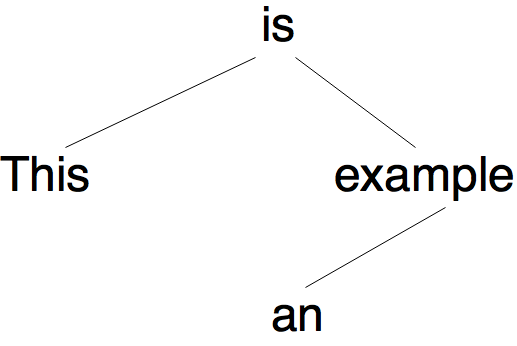
\includegraphics[scale=0.4]{DependencyTree.png}
   \caption[An example of a Dependency Tree]{A possible dependency tree for the sentence \emph{This is an example}.}
   \label{dependencyTree}
\end{figure}

In the tree (Figure \ref{dependencyTree}), the word \emph{This} is dependent on \emph{is} and so is linked. \emph{an} is linked to \emph{example} in a similar way, and \emph{an example} is dependent on the verb \emph{is} and so also has a link to it. 

Once dependency trees have been created for each of the sentences a similarity algorithm is used to find sentences that are similar. The common phrases between these similar sentences are then taken and form the basis of the final summary. A language generator then combines the common phrases and arranges it to create a final set of summary sentences.

An obvious disadvantage to this method is that if only common phrases are taken from the sentences, context could be lost from some of the sentences. However, on the other hand, the use of a language generator means that a more coherent, more grammatically correct summary is formed. \\

\emph{Rule based summarisation}\index{Summarisation!Rule based}

In rule based summarisation \cite{ruleBasedSummarisation}, the process is centred around a list of pre-determined categories. With each of these categories, there is a pre-determined set of questions to be answered. 

For example, with a theoretical category \emph{Product Launch} we could have the following questions:

\begin{enumerate}
	\item What is the name of the product?
	\item What company is launching it?
	\item What type of product is it?
	\item What's new about it?
	\item What price is it retailing at?
\end{enumerate}

This represents only a subset of the possible questions we could have for this category.

To perform rule based summarisation, the first step is to analyse the document and determine which category it fits best. Once that's been determined, the next stage is to analyse the text to find answers to the questions corresponding to that category. These answers are then fed in to a natural language generator that forms sentences, and thus the summary.

Results for this method of abstractive summarisation have been promising, but the method has a major disadvantage in that the list of categories and questions needs to be pre-determined. As a result, it might not be an optimal algorithm to use for the ever-changing world of news reporting. \\

\emph{Ontology based summarisation}\index{Summarisation!Ontology based}

Methods of ontology based summarisation have been developed, primarily using domain based ontology. In this method a "domain expert" defines a domain ontology for a news event. Each new document is then classified into a topic using these domain ontologies\index{Domain Ontology}. Important phrases are determined by how close they are to items in the ontology. These phrases are then passed into a natural language generator to form the final summary sentences.

A key disadvantage to this method is that a lot of the domain ontologies has to be manually determined by the "domain experts" and so can be very time consuming. As a result this may also not be particularly optimal for summarisation of news events. \\

\textbf{Semantic based summarisation} \\

\emph{Multimodal Semantic summarisation}\index{Summarisation!Multimodal Semantic}

Multimodal semantic summarisation can work on documents that contains both text and images. First, a semantic model is built to represent the document. This model is made up of different concepts that are surmised from the text. For example, the sentence \emph{Multimodal Semantic summarisation is an example of an algorithm that performs abstractive summarisation}\index{Summarisation!Abstractive} could form the concept shown in Figure \ref{multimodalSummarisation}:

\begin{figure}[ht!]
  \centering
    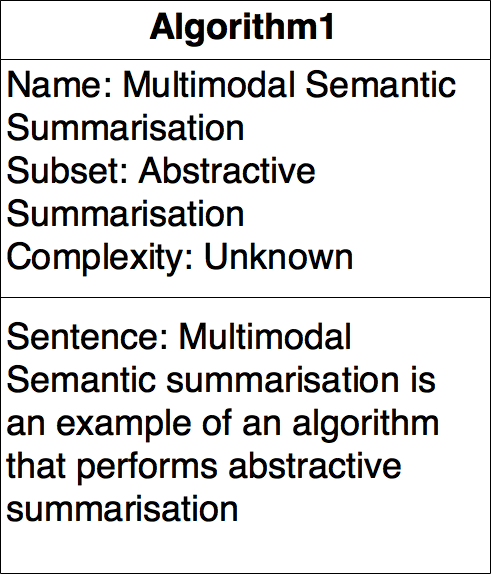
\includegraphics[scale=0.3]{MultimodalSummarisation.png}
   \caption[A concept created during multimodal semantic summarisation]{A possible concept created from the analysis of the sentence \emph{Multimodal Semantic summarisation is an example of an algorithm that performs abstractive summarisation}.}
   \label{multimodalSummarisation}
\end{figure}

Concepts\index{Concept!Multimodal Summarisation} are gradually filled with more information as the entire text is analysed. Links are also added between concepts that share some relationship. For example in Figure \ref{multimodalSummarisation} if there was another sentence that surmised a concept called \emph{Abstractive Summarisation} then there would be a link from \emph{Algorithm1} to that new concept. 

The next step is to rank the concepts. This is done by taking into account the completeness of the concept, and the number of links that the concept as to others. This way, the concepts are ranked by which is most important to the original document. Once the key concepts have been identified summary sentences can be generated featuring these concepts. \\

\emph{Information Item based method}\index{Summarisation!Information Item}

Information Item based summarisation \cite{informationBasedSummarisation} relies on the content of the summary being determined from an abstract representation of the original document, rather than the sentences from the document themselves. To do this, the document is first scanned so that Information Items (InIt) can be generated. An information item is defined as being "the smallest element of coherent information in a text or sentence". 

Once the information items have been created, they are then ranked using frequency analysis to find the most important predicates and entities from the original document. This step is near identical to the term frequency stage in extractive summarisation (Section \ref{extractiveSummarisation})\index{Summarisation!Extractive}. These information items that are ranked highly are then combined and fed into a natural language generator to form the final summary sentences. \\

\emph{Semantic Graph summarisation}\index{Summarisation!Semantic Graph}

Semantic Graph summarisation centres around a rich semantic graph (RSG)\index{Rich Semantic Graph}. The document is first converted into a RSG. Each node in the RSG represents a noun or verb in the document, and the links between the nodes represent the semantic and topological relations between these nouns and verbs. In the second stage, heuristic rules are used to reduce the semantic graph to a more minimalistic version. This will form the basis of the final summary. In the final step, the minimised RSG is passed into a generator that creates the final summary sentences.

The steps are outlined in the flowchart provided in Figure \ref{semanticGraphSummarisation}.

\begin{figure}[ht!]
  \centering
    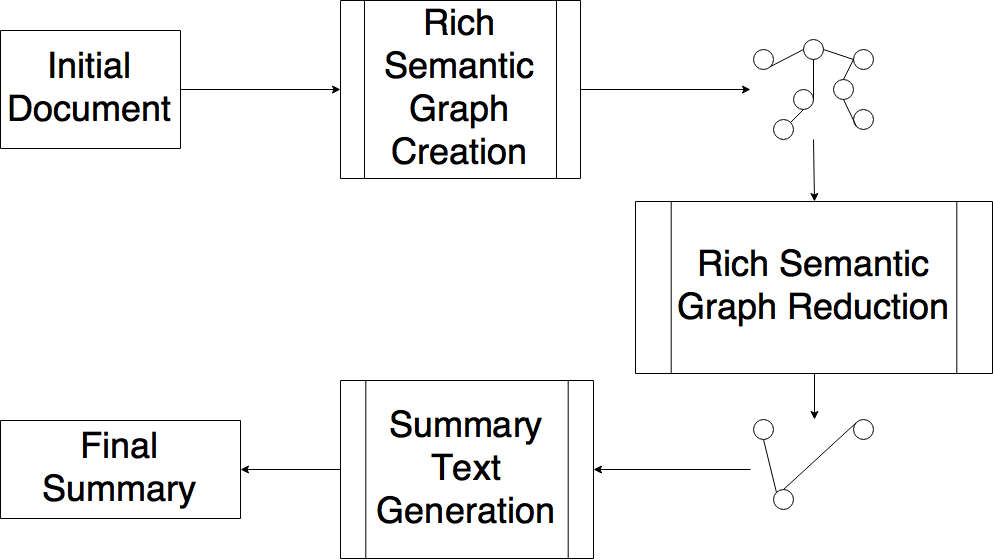
\includegraphics[scale=0.4]{SemanticGraphSummarisation.png}
   \caption[A flowchart showing the process of semantic graph summarisation]{This shows the process of semantic graph summarisation in a flowchart based on those provided in  \cite{abstractiveTechniques, abstractiveTechniquesOriginal}.}
   \label{semanticGraphSummarisation}
\end{figure}

Semantic Graph summarisation has had success with producing an abstractive summary that has fewer redundant sentences, and is also good at producing grammatically correct sentences. However, it's only designed for use with a single document as input. As a result it might not be suitable as a method for summarising the multiple documents needed for the aggregator, unless it's combined with another method.

\subsection{Natural Language Processing Libraries} 

A lot of the summarisation techniques specified earlier, especially for abstractive summarisation, would require a full analysis of the semantics of a body of text. As a result, it's clear that a Natural Language Processing library will be needed for this task.

Writing in the LA Times \cite{latimes}, in his article \emph{Natural Language Processing in the kitchen} \cite{nlpkitchen}, Anthony Pesce says "Natural Language Processing is a field that covers computer understanding and manipulation of human language, and it's ripe with possibilities of for newsgathering. You usually hear about it in the context of analyzing (sic) large pools of legislation or other document sets, attempting to discover patterns or root out corruption."

Therefore, a Natural Language Processing (NLP) library could you be used for various aspects of summarisation, as well as potentially in areas such as clustering and labelling. With this in mind I started to do some research in the area to identify what features could prove useful going forward.

\subsubsection{Aspects of Natural Language Processing} 

\label{nlptypes}

There are several different tasks that a Natural Language Processor \cite{nlpwiki}. A few key ones that are most likely to be required for the project are explained briefly below: 

\begin{itemize}
	\item \textbf{Tokenisation} is the splitting of words in a given document. 
	\item \textbf{Sentence Segmentation} is the splitting of sentences in a given document. 
	\item \textbf{Part-of-Speech (POS) tagging} takes a list of tokens and analyses them, returning tags for each. A tag represents the grammatical function of the token in the sentence (for example if it is a noun, verb or adjective). 
	\item \textbf{Named entity extraction} identifies the proper nouns within a document, such as people, dates or locations, as well as other categories of noun. 
	\item \textbf{Chunking} takes a list of tags from a POS tagger and groups sets of tokens by their function in a sentence. Examples can include noun phrases and verb phrases. 
	\item \textbf{Parsing} takes a sentence and develops a tree showing the functions of each Section of the sentence. 
	\item \textbf{Coreference Resolution} identifies noun phrases within a document that are the same. This can commonly be used for replacing pronouns with the original noun phrase. 
\end{itemize}

\subsection{Conclusions}

After conducting the background research I was able to come up with the following basic conclusions as to how to lead in to the design phase of the project.

\begin{itemize}
	\item In \textbf{Topic Modelling} (Section \ref{TopicModellingTechniques}) the better initial approach will be to employ (or to use a library that employs) Latent Dirichlet Allocation (LDA) as opposed to Latent Semantic Indexing (LSI). LDA uses a generative probabilistic model, which has in practice produced significantly more accurate results. Time shouldn't be of much concern in this case, as the model won't have to be generated very often. As a result, LSI's major advantage is rendered irrelevant.
	\item For \textbf{Topic Labelling} (Section \ref{labellingalgorithm}) following the algorithm set out by Lau, Grieser, Newman Baldwin \cite{topicLabelling} would be the best option, as it has had strong success in its methods (although admittedly this is their own claim). A potential issue to consider however is that the algorithm would require several (and perhaps dozens) of calls to Wikipedia \cite{wikipedia}. This could be time intensive.
	\item With \textbf{Clustering} (Section \ref{ClusteringTechniques}), there are significant disadvantages with the techniques of centroid clustering and density clustering. With the first, the number of clusters need to be known, and with density clustering accuracy can be lower than needed. Out of the two hierarchical clustering approaches, agglomerative would probably be the most useful, as it could be slightly faster than a top-down divisive approach. A vector score based on Term Frequency-Inverse Document Frequency \cite{tfidf} is a tried and tested metric for clustering, and will also come in handy.
	\item For \textbf{Summarisation} (Section \ref{summarisation}), a combination of extractive and abstractive summarisation would probably be best. The LexRank \cite{lexRank} approach for extractive summarisation could help combine the multiple articles into one document, which could then be fed into the semantic graph abstractive summarisation algorithm \cite{abstractiveTechniques, abstractiveTechniquesOriginal}.
	\item \textbf{Natural Language Processing}, (Section \ref{nlptypes}) will come in handy, especially in the summarisation phase. For example, with abstractive summarisation, it could be used to analyse the grammatical structures of the text in the semantic graphing phase.  
\end{itemize}

%%%%%%%%%%%%%%%%%%%%%%%%%%%%%%%%%%%%%%%%%%%%%%%%%%%%%%%%%%%%%%%%%%%%%%%%%%%%%%%%%%%%%%%%%%%%%%%%

\newpage

\section{Design}

In this section I set out the overview of the design for the product. There are three important aspects to consider. 

\begin{itemize}
	\item How the front end should look, and what the underlying infrastructure and flow of it should be. 
	\item The back end, and more importantly the process of an article being summarised, starting with taking an article from an outlet and going all the way until the summary itself is generated. 
	\item The infrastructure of the back end, namely the storage system and the company used to host the server. 
\end{itemize}

\subsection{Front End Architecture\index{Front End}\index{Architecture} Diagram}

\begin{figure}[ht!]
  \centering
    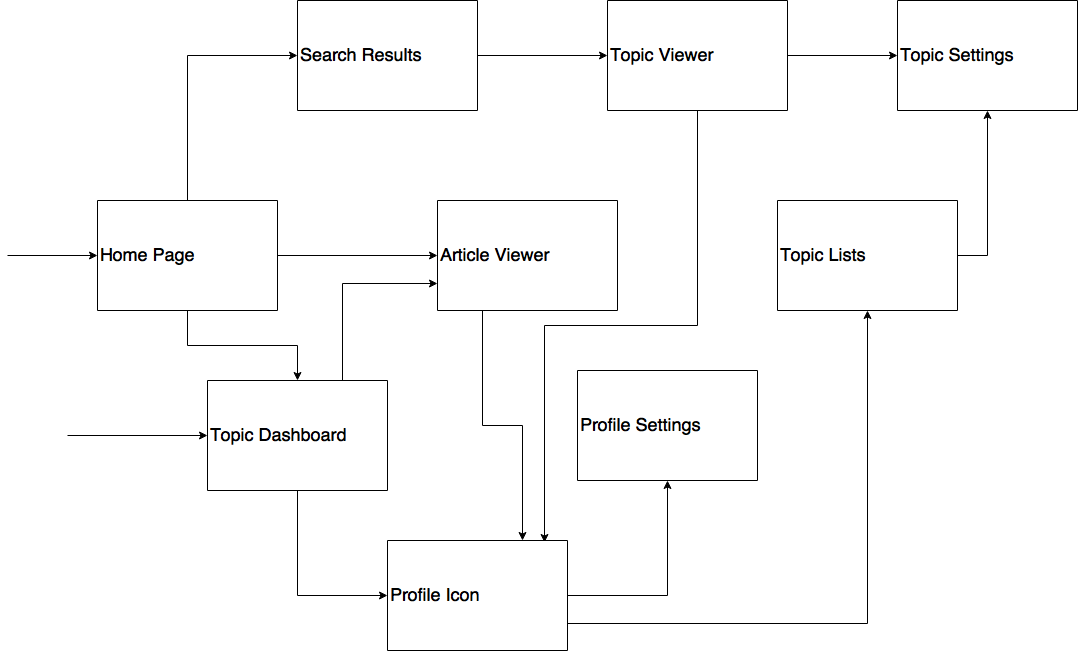
\includegraphics[scale=0.4]{FrontEndArchitecture.png}
   \caption[A basic diagram of the expected architecture of the front end]{A diagram showing the expected architecture of the front end application.}
   \label{frontEndArchitecture}
\end{figure}

Figure \ref{frontEndArchitecture} depicts the expected flow for the front end. A navigation bar will be present on all screens, and will provide links to the Home Page (Section \ref{homepage}), the Topic Dashboard (Section \ref{topicdashboard}) and Settings pages (Appendix \ref{topicsettings}). 

From the Home Page, the user can search for a topic, taking them to the Search Results screen (Appendix \ref{searchresults}). They can alternatively click on one of the latest articles, which will in turn take them to the Article Viewer (Section \ref{articleviewer}).

Both the Topic Dashboard and the Search Results screen will display a list of topics in some form - in the case of the dashboard, it will be a list of the user's subscriptions, and in the latter a list of search results. They thus both have a direct link to the Topic Viewer (Appendix \ref{topicviewer}), which can be accessed by clicking on one of the items in the list.

The Topic Viewer presents the articles for the topic, and clicking on one will take the user to the aforementioned Article Viewer.

The Topic Settings screen is a standalone screen accessible from the Navigation Bar on any page.

\subsection{User Story}

\label{userstory}

In the following the designs and justifications for the Home Page, Topic Dashboard and Article Viewer screens are presented. Other screens, including the Search Results screen, Topic Viewer and Topic Settings pages can be found in Appendix \ref{wireframes}.

\subsubsection{Home Page}

The first page that a consumer will see on the website is the Home Page (Figure \ref{homePage}). The key to the design of the home page is that it's easy to get started for a user. They are presented with a large search box that they can use without having to sign in. There'll also be a row of trending articles displayed below the search bar. This row will consist of icons consisting of images and titles below, as shown in the wireframe\index{Wireframe} of Figure \ref{homePage}. There's a navigation bar at the top, that is present on all screens, with a button to register and a button to sign in on the top right, and a link to information about the application itself on the top left.

\label{homepage}

\begin{figure}[ht!]
  \centering
    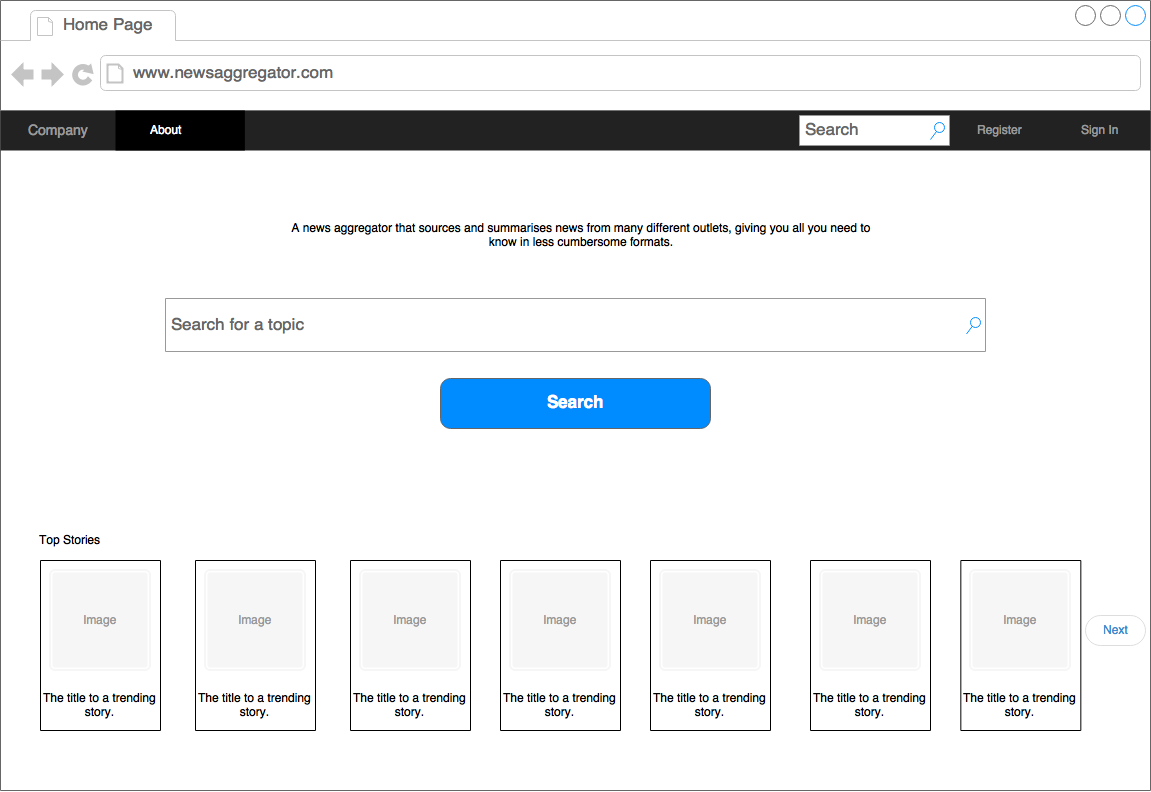
\includegraphics[scale=0.3]{HomePage.png}
   \caption[A wireframe of the Home Screen]{A key focus of the home page is that the user can easily search for articles without having to sign in or register.}
   \label{homePage}
\end{figure}

\subsubsection{Topic Dashboard}

Clicking on the "My Topics" button in the navigation bar will take the user to the Topic Dashboard, assuming they have logged in. If they haven't, they will first be prompted to log in. Here the user can see all the topics that they have subscribed to. As shown in Figure \ref{topicDashboard}, there is a section showing the various articles in a topic, along with a tab bar at the bottom indicating the topics that a consumer is subscribed to. They can drag to one direction (akin to a sideways swipe on a phone or tablet) to see articles pertaining to the next topic. 

Articles themselves are presented as panels. On a panel is an image for the article, with the title overlaid. In the top right hand corner are icons corresponding to the sources that the article has been summarised from. Leading articles (those out of the most recent that have the most sources attached) are placed in the larger panels on the top left and bottom right of the screen, as shown in the diagram.

\label{topicdashboard}

\begin{figure}[ht!]
  \centering
    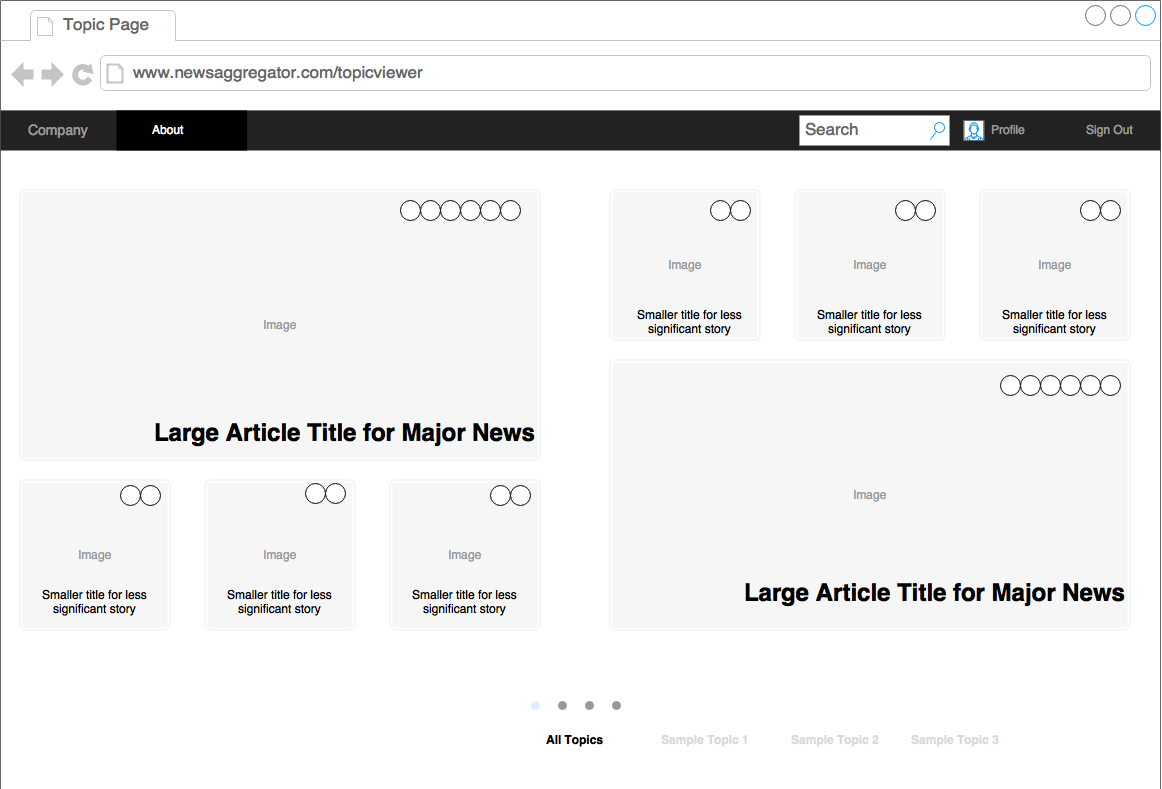
\includegraphics[scale=0.3]{TopicDashboard.png}
   \caption[A wireframe of the Topic Dashboard]{The topic dashboard has the ability to show articles across all topics, or pertaining to a specific topic.}
   \label{topicDashboard}
\end{figure}

\subsubsection{Article Viewer}

When the user clicks on an article panel in the topic viewer or topic dashboard they are presented with the summarised article itself. This screen (Figure \ref{articleViewer}) is modelled on standard news interfaces, and produces the headline, image and article body on the left hand side of the page. On the right hand side are links to the original articles that the summary was generated from, and links to other articles that are in the same topic. 

Like most other screens in the application, there is also a share button on the top right, and an email button.

\label{articleviewer}

\begin{figure}[ht!]
  \centering
    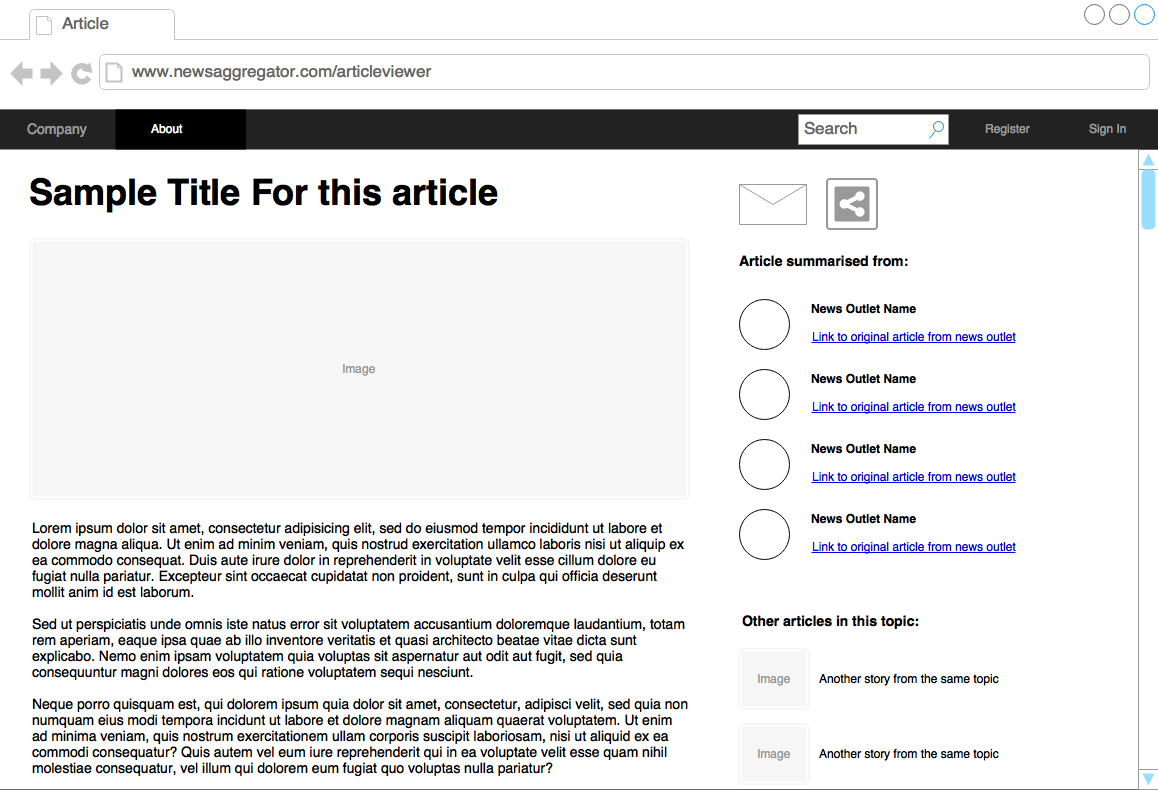
\includegraphics[scale=0.3]{ArticleViewer.png}
   \caption[A wireframe of the Article Viewer]{The Article Viewer is modelled on standard news outlets' interfaces.}
   \label{articleViewer}
\end{figure}

\subsection{Back End\index{Back End} Flow Diagram}

In Figure \ref{backEndArchitecture} the expected flow of the machine learning aspects of the back end is presented. The process of an article being summarised is as follows:

\begin{enumerate}
	\item The \textbf{Article Fetcher} queries the various News APIs used for new articles. 
	\item The \textbf{Article Curator} takes the response from the News APIs and performs any scraping that may be necessary, before passing the article to the Machine Learning phases. 
	\item The article is then passed to the \textbf{Topic Modelling}\index{Topic Modelling} phase, which identifies which topics it consists of. 
	\item The \textbf{Topic Labelling}\index{Topic Labelling} Section takes the results of the Topic Modelling phase, and proceeds to label its topic. 
	\item \textbf{Clustering}\index{Clustering} then occurs. The article, along with its topic label is passed to this phase, and the program pulls articles from the database that have already been assigned the same topic. These articles are then clustered, and the cluster containing this article is passed to the next phase. 
	\item Now that the cluster has been passed, \textbf{Summarisation}\index{Summarisation} occurs on the article, which is then put in the Summarised Articles database, ready to be called for a user to read. 
\end{enumerate}

\begin{figure}[ht!]
  \centering
    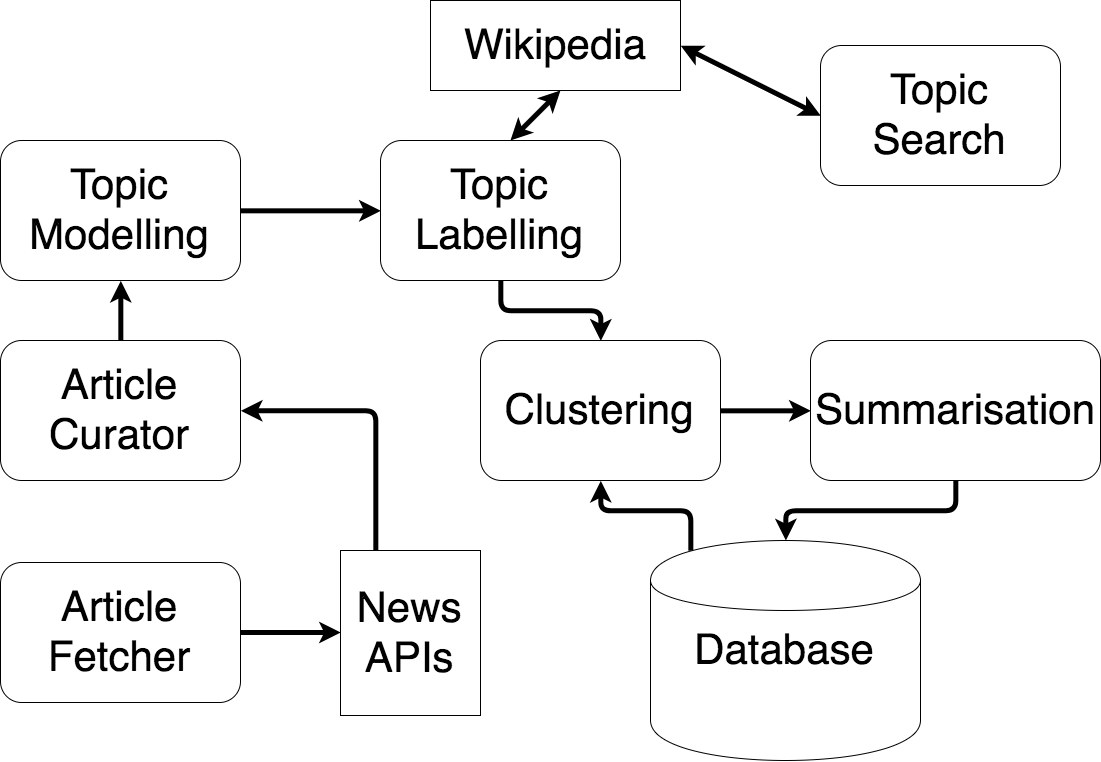
\includegraphics[scale=0.4]{BackEndArchitecture.png}
   \caption[A guide to the expected flow of the Back End]{The expected flow of the Back End.}
   \label{backEndArchitecture}
\end{figure}

\subsection{Infrastructure}

\subsubsection{Hardware}

One of the first key decisions I made about the infrastructure surrounded the hardware that the server would be deployed on.

\textbf{Amazon Web Services}

Amazon Web Services (AWS) \cite{aws} is a set of cloud computing platforms provided by Amazon \cite{amazon}. A key benefit to it is that it has a free tier, which allows for a subset of their services to be used without charge.

Some of the key platforms offered by AWS include: \\

\begin{itemize}
	\item \textbf{EC2} \cite{ec2} allows a user to create a single virtual machine for free on which to run software. This would be with a limit of 750 hours of use per month. In my case this would be used for running the back end of the News Aggregator. 
	\item \textbf{S3} \cite{s3} is a storage system provided by Amazon that allows a user 5GB of space for free. \\
\end{itemize} 

\textbf{Digital Ocean}

Digital Ocean \cite{digitalOcean} is an infrastructure provider that provides "cloud computing for developers". Digital Ocean offers "droplets" that can act as virtual machines, on which I would deploy my backend. There are no free tiers, but the student pack provided by GitHub \cite{github} would cover the first two months of charges. 

In addition to this, one of the advantages of Digital Ocean is that if resizing of the virtual machine is necessary, it can be done in a matter of minutes, thus making the final solution very highly scalable.

In contrast though, unlike Amazon, Digital Ocean don't provide alternative microservices such as S3. Having said that, it could be argued that the droplet itself would offer that with its storage capabilities. In fact, the cheapest droplet offered by Digital Ocean (priced at \$5 a month), entails a virtual machine with a 20GB SSD disk, which is four times the amount provided by the free tier in AWS.

\subsubsection{Database}

\textbf{MongoDB}

The first database solution that I researched was MongoDB \cite{mongodb}, as I have had prior experience with it. 

MongoDB is a document database that is designed to be both flexible and highly scalable. Documents are written in a format that is highly similar to JSON. This format is what results in a Mongo database being flexible, as the schema of documents in the collection can be changed quickly. 

MongoDB allows for the connection of items between tables through linking. Auto-generated "ObjectId"s (that are generated based on the timestamp) allow for easy referencing of an item in another.

A MongoDB database would have to remain in a virtual machine on either Amazon or Digital Ocean, and will therefore have to count against the storage provided by that virtual machine. \\

\textbf{DynamoDB}

DynamoDB \cite{dynamodb} is a No-SQL database provided by Amazon Web Services as a separate micro-service to EC2 and S3. 

The structure of a document in DynamoDB is more rigid than in MongoDB. It is primarily designed as a key-value system, with a primary key. Searching in the database is driven by this primary key, or by "secondary indexes". These secondary indexes need to be declared when the table is first created. Therefore this means that if there needs to be a schema change, the table needs to be recreated.

A DynamoDB database doesn't need to be stored in the virtual machine, but there are trade offs. Whilst Amazon Web Services provide 25GB of storage for the database as part of the free tier, there are throttles on the throughput of the database. As part of the free tier, a user is allowed to allocate 25 "units" of throughput to both reading and writing from a database, where one unit corresponds to transfer of 1KB per second. Beyond these 25 units, Amazon would start charging.

\subsubsection{Infrastructure Decisions}

\textbf{Comparison table}

Table \ref{infrastructuretable} shows the key points of comparison between the four main options for hardware and database combinations. \\

\begin{sidewaystable}
    \begin{tabular}{p{4.5cm}|p{7.75cm}|p{7.75cm}}
    \textbf{Infrastructure} & \textbf{Advantages} & \textbf{Disadvantages} \\ \hline
    AWS and MongoDB & \tabitem AWS provide free services & \tabitem Mongo would need to be hosted on the EC2 instance, or on S3, which would limit the free storage to 5GB. \\ & \tabitem Mongo provides a flexible schema, meaning that the table structure can be changed further down the line.  \\ \hline
    AWS and DynamoDB & \tabitem DynamoDB would provide 25GB of storage on its own, meaning that I wouldn't have to use the S3 storage. & \tabitem DynamoDB's key-value schema is quite rigid, meaning that there isn't much flexibility on the model.\\ & & \tabitem The throttling of reads and writes by DynamoDB could severely impact the performance of key back end tasks.\\ \hline
    Digital Ocean and DynamoDB & \tabitem Digital Ocean offers the ability to resize the server as needs be within a matter of minutes. & \tabitem As before, there are some key issues regarding the speed of DynamoDB whilst on the free tier. \\ & &\tabitem This solution would involve maintenance of a database solution provided by one company, and a server on another, which is potentially quite wasteful.  \\ \hline
    Digital Ocean and MongoDB & \tabitem MongoDB database can be stored comfortably on the Digital Ocean droplet & \tabitem Whilst covered by vouchers for the first two months of use at least, the Digital Ocean instance would require expenditure if used for longer than that period, versus AWS EC2 which would be free for at least twelve months.\\ & \tabitem The flexibility of the MongoDB model would mean that fields can be removed and added easily from the schema, allowing for further changes down the line. \\
  \end{tabular}
  \caption[Advantages and Disadvantages of different Infrastructure combinations]{Comparing the advantages and disadvantages of potential combinations of hardware and database options.}
  \label{infrastructuretable}
\end{sidewaystable}


\textbf{Decision Process}

I tried all possible combinations listed in table \ref{infrastructuretable} before finally arriving at the decision of using Digital Ocean and MongoDB.

I initially started with the configuration with AWS and MongoDB. However, it became clear quite quickly that there was a distinct possibility that the memory provided by AWS would not be sufficient to hold a large number of articles (about six weeks or greater) in the database. There certainly would not be scope for adding extra outlets near the end of the project.

In an attempt to counter this, and trying to avoid solutions that would require the spending of money, I then switched the database option to DynamoDB. This worked well for a time, but as the database grew, it became clearer that the throttling of the read and write operations to my database was going to cause major issues down the line for my background jobs on the server, as well as for simple API methods. In order to counteract this, I resolved that I would use vouchers for AWS from the GitHub student pack in order to fund some extra read-write operations per second.

Having resolved to do this, I then decided to make use of Digital Ocean. This was because I wanted to experiment to see the effects of having an instance with extra RAM on the running of my program, and knew that the vouchers on the GitHub student pack would easily cover a Digital Ocean droplet until the end of the project. What I found was that my background jobs (such as pulling in articles, labelling, clustering and summarisation) were being performed faster in general, and so I decided to permanently move to Digital Ocean.

In the end, a final nail in the coffin for my use of Amazon Web Services came when I wanted to change the way my articles table worked in the database. I had wanted the ability to search by date published (as I was considering at the time removing articles published before a certain date), but found that I would have to recreate my entire table in order to add this functionality to my table. As a result, and combined with the fact I now had a much larger amount of storage space on my new Digital Ocean droplet, I took the decision to make a new MongoDB database, knowing that it was still early enough in the development process that losing all my previous database work would not affect the finished product, or the development timeline.



%%%%%%%%%%%%%%%%%%%%%%%%%%%%%%%%%%%%%%%%%%%%%%%%%%%%%%%%%%%%%%%%%%%%%%%%%%%%%%%%%%%%%%%%%

\newpage

\section{Implementation}

Having established the basic design of the front end of the application, and the platforms to be used for the server and database, I moved on to the implementation. In this section I present my ideas and justifications for language choices (Section \ref{languagechoice}), the schema for the database (Section \ref{database}), and use of specific APIs and libraries (Sections \ref{apis} and \ref{libraries}).

In the latter parts of the implementation section, I also present in detail my algorithms for the machine learning and summarisation aspects (Section \ref{machinelearning}).  

\subsection{Language Choices}

\label{languagechoice}

\subsubsection{Front End}

The survey\index{Survey} that was conducted in Section \ref{survey} clearly presented the result that a website would be the preferred option for the application, followed by a mobile application in iOS. Therefore I've decided to follow this and create a WebApp as a primary platform. I'll then develop the application for a second platform, which will be iOS.

For the WebApp I will primarily use Bootstrap \cite{bootstrap} for the Interface. One design framework I used to great effect during my Industrial Placement in Summer 2016 was React \cite{react} and Redux \cite{redux}\index{Redux}\index{React}. React is a JavaScript library developed by Facebook \cite{facebook} that is designed for building scalable and reusable user interfaces. Redux is a design pattern for JavaScript that is designed around a central predictable state container that is the single source of truth for a User Interface. 

The benefit of this framework is that it allows for very clean code in the user interface. This is because the concept of a single source of truth allows for data flow that is purely in only one direction, making it easier to understand.

\subsubsection{Back End}

The back end will be constructed using Java. The reasoning behind this is that I have experience from my Industrial Placement using Java as the basis of a server and a back end.

\subsection{Database Schema}

\label{database}

\subsubsection{Schema Diagram}

Figure \ref{dbschema} shows the basic components of the various collections in the Mongo Database \cite{mongodb}, along with some of the connections involved. Further details on each are given in each of the following sections.

\begin{figure}[ht!]
  \centering
    \includegraphics[width=\textwidth]{DBSchema.png}
   \caption[A diagram of the MongoDB schema]{A diagram of the core MongoDB schema.}
   \label{dbschema}
\end{figure} 

\subsubsection{Articles}

A sample document for an article can be seen below:

\begin{lstlisting}[language=json, firstnumber=1, caption={A sample document in the Article table},captionpos=b]
{
    "_id" : ObjectId("591df7cfacea820abe29709f"),
    "Title" : "Kirsten, Simons on five-man panel in hunt for new SA coach",
    "Body" : "Cricket South Africa has nominated a five-man panel including two former national coaches, Gary Kirsten and Eric Simons, to recommend a suitable candidate for the position of head coach, which it aims to fill by the beginning of September
    ...
    ",
    "ImageURL" : "http://www.espncricinfo.com/db/PICTURES/CMS/157600/157626.5.jpg",
    "ArticleURL" : "http://www.espncricinfo.com/southafrica/content/story/1098337.html",
    "Source" : "espn-cric-info",
    "LastPublished" : "2017-05-18T10:42:38Z",
    "isLabelled" : true
}
\end{lstlisting}

The purpose of the article table is for storage of raw article data that has been brought in by the article fetcher. Most fields are self explanatory. The \emph{isLabelled} field is defaulted to false when an article is first brought in, and is then changed to true when the Topic Labeller has labelled it. This is present so that articles that either weren't labelled, or caused an error when being labelled, can be found with a simple search in the database.

\subsubsection{Topics}

A sample document for a topic can be seen below:

\begin{lstlisting}[language=json, firstnumber=1, caption={A sample document in the Topics table},captionpos=b]
{
    "_id" : ObjectId("591df830acea820aebf55465"),
    "Label" : "Opposition (politics)",
    "Articles" : [ 
        ObjectId("591e172dacea820aebf55a74"), 
        ObjectId("5925f959acea821a75b831bc"), 
        ObjectId("59281cddacea821ab611d3ed"), 
        ObjectId("59291a47acea82594af9ef53"), 
        ObjectId("592aa5daacea8264125210d3")
    ],
    "Clusters" : [ 
        ObjectId("591f8bc7acea821e031f4dc6")
    ],
    "NeedsClustering" : true,
    "imageUrl" : "https://upload.wikimedia.org/wikipedia/commons/d/d1/Stand_in_opposition_city_hall_boston.jpg"
}
\end{lstlisting}

A topic object is a core concept in the back end. It keeps references to all articles that have been labelled with that topic, and also holds references to all the clusters (summaries) that are produced from these articles. The \emph{imageUrl} field holds either the lead image for the corresponding Wikipedia \cite{wikipedia} article, or a placeholder if the Wikipedia article doesn't have an image. 

The \emph{NeedsClustering} flag performs a similar function to the \emph{isLabelled} flag in the Articles table. It is defaulted to true, and is changed to false once all the clustering (but not necessarily summarisation) is completed. It is used again to find topics that may have "slipped through the cracks", either due to an error, or for some other reason. 

\subsubsection{Clusters}

A sample document for a cluster can be seen below:

\begin{lstlisting}[language=json, firstnumber=1, caption={A sample document in the Summaries table},captionpos=b]
{
    "_id" : ObjectId("591e47f7acea8221dcb97c42"),
    "Articles" : [ 
        ObjectId("591df7cfacea820abe2970a9"), 
        ObjectId("591df7cfacea820abe2970b2")
    ],
    "Summaries" : "{\"[http://www.cnn.com/2017/06/01/politics/trump-paris-climate-decision/index.html,http://www.reuters.com/article/us-usa-climatechange-eu-idUSKBN18S5IT]\":[{\"sentence\":\"BRUSSELS The European Union said on Thursday it had made its position on climate change clear and was not engaged in last-minute lobbying of the Trump administration to keep the United States aboard the Paris climate accord.\",\"sentencePosition\":0.0,\"absoluteSentencePosition\":0,\"identifier\":26,\"relatedNodes\":[],\"source\":\"reuters\"}
    ...
    ]}"
}
\end{lstlisting}

An object in this table represents a Summary, and corresponds to the Clusters array in a Topic. It contains an array of references to the original articles used for the summarisation.

The \emph{Summaries} field is a string representation of a map object, with the values representing to a summary, and the corresponding key representing a combination of articles used to make that summary (represented using their URLs). For example, in the full version of the sample document, there would be three keys in the string representation:

\begin{sloppypar}
\begin{itemize}
	\item \textbf{[http://www.cnn.com/2017/06/01/politics/trump-paris-climate-decision/index.html,http://www.reuters.com/article/us-usa-climatechange-eu-idUSKBN18S5IT]{}}, for a summary using articles from \emph{CNN} and \emph{Reuters}.
	\item \textbf{[http://www.cnn.com/2017/06/01/politics/trump-paris-climate-decision/index.html]}, for a summary using an article from \emph{CNN}.
	\item \textbf{[http://www.reuters.com/article/us-usa-climatechange-eu-idUSKBN18S5IT]}, for a summary using an article from \emph{Reuters}. \\
\end{itemize}
\end{sloppypar}

These represent all the possible permutations (of size greater than zero) of the articles in the cluster. Its primary use is in the customisation offered to users, that can be seen in more detail in Section \ref{frontendimplementation}.

\subsubsection{Users}

A sample document for a User can be seen below:

\begin{lstlisting}[language=json, firstnumber=1, caption={A sample document in the Users table},captionpos=b]
{
    "_id" : ObjectId("592c5288acea82147ca7f0d1"),
    "emailAddress" : "fake@gmail.com",
    "topicIds" : "[{\"topicId\":\"591e3c74acea821e2b7e6c02\",\"sources\":[\"wikipedia\",\"business-insider-uk\",\"daily-mail\",\"espn-cric-info\",\"metro\",\"mirror\",\"newsweek\",\"sky-sports-news\",\"the-telegraph\",\"the-times-of-india\",\"bbc-news\",\"bbc-sport\",\"bloomberg\",\"cnn\",\"cnbc\",\"espn\",\"four-four-two\",\"the-washington-post\",\"the-wall-street-journal\",\"associated-press\",\"the-guardian-uk\"],\"digests\":false}]"
}
\end{lstlisting}

A user object is very simple. The only field that is not necessarily self-explanatory is the \emph{topicIds} field. 

This is an array of strings, with each string forming a representation of a user's topic subscription (the topic being represented by the field marked \emph{topicId}), and the settings for that topic. The two core settings for each subscription is the digests setting (a boolean flag indicating whether a user wants to receive email digests that include this topic), and a list of sources that the user would like their news to default to (further information on this feature can be seen in Section \ref{frontendimplementation}). By default, when a user subscribes to a topic, defaults is set to false, and sources is represented by a list comprising all possible sources.

\subsubsection{Digests}

A sample document for a digest can be seen below:

\begin{lstlisting}[language=json, firstnumber=1, caption={A sample document in the Digests table},captionpos=b]
{
    "_id" : ObjectId("591ec5c433625db581d77cc6"),
    "id" : "591ec5c433625db581d77cc6",
    "articleHolders" : "[{\"topicId\":\"593020de5826a72aa697a201\",\"articleId\":\"59322bc5acea820dd0c7ef37\",\"title\":\"Elon Musk 'intrigued' by India's objective of all-electric cars by 2030 - Times of India\",\"imageUrl\":\"http://timesofindia.indiatimes.com/photo/msid-58964385/58964385.jpg?53722\",\"lastPublished\":\"2017-06-03T08:40:00Z\"},{\"topicId\":\"5930210d5826a72aa697a227\",\"articleId\":\"59324084acea820dd0c7f65b\",\"title\":\"Kathy Griffin loses ALL of her tour gigs in wake of Trump scandal\",\"imageUrl\":\"http://i.dailymail.co.uk/i/pix/2017/06/03/05/410C672100000578-0-image-a-41_1496464334669.jpg\",\"lastPublished\":\"2017-06-03T04:39:14Z\"},{\"topicId\":\"593020de5826a72aa697a201\",\"articleId\":\"59323dddacea820dd0c7f566\",\"title\":\"Putin says hacking of Democratic Party may have been CIA false flag op\",\"imageUrl\":\"http://i.dailymail.co.uk/i/pix/2017/06/03/05/410C6AD500000578-0-image-a-92_1496463783859.jpg\",\"lastPublished\":\"2017-06-03T04:28:04Z\"}
    ...
    ",
    "emailAddress" : "specialk109@gmail.com"
}
\end{lstlisting}

A digest document represents a single daily digest for a user. Thus, a user who gets daily digests would have a single object for each day. Having said a user would have a single object for each day, it's worth pointing out that the digests are not linked to the User object. Whilst there is no concrete justification for this to be the case either way, a reason for the digests table and users table to not be linked in some way is that they simply don't need to be. A user is never called when a digest is retrieved, and similar a digest is never called when a user is retrieved.

The \emph{articleHolders} field in the document above represents the articles in a digest. It is an array of strings, with each string a JSON representation of an object containing a topic id, article id, and basic information about the cluster (title, image url, and a publishing date). The reasoning behind having the topic id in addition to the cluster is due to the pattern matching employed in the URL for the article viewer on the website (this is explained in further detail in Section \ref{frontendimplementation}).

\subsection{Useful APIs}

\label{apis}

\subsubsection{News Outlets}\index{News!Outlets}

\textbf{Readership statistics for selected outlets in the United Kingdom\index{United Kingdom}}

Statistics below are taken from the \emph{Digital News Report 2016} \cite{digitalNewsReport}\index{Digital News Report} by the Reuters Institute for the Study of Journalism \cite{reutersInstitute}\index{Reuters Institute for the Study of Journalism}. Viewership is given as a percentage of people who say they use the outlet at least weekly.

\begin{table}[H]
	\centering
	\begin{tabular}{l|c|r}
		\textbf{Outlet} & \textbf{Viewership} &\textbf{Political Stance} \\ \hline
		BBC\index{BBC} & 51\% & Neutral \\ \hline
		Mail Online\index{Mail Online} & 17\% & Right \\ \hline
		Huffington Post\index{Huffington Post} & 14\% & Left \\ \hline
		The Guardian & 14\% & Left \\ \hline
		Sky News Online\index{Sky News} & 11\% & Neutral \\ \hline
		The Telegraph Online\index{Telegraph, The} & 9\% & Right \\ \hline
		The Independent\index{Independent, The} & 6\% & Centrist \\ \hline
	\end{tabular}
	\caption[Readership statistics for selected UK outlets]{Readership statistics for selected outlets in the United Kingdom.}
	\label{viewershipFigures}
\end{table}

\textbf{\\The Guardian }

\emph{The Guardian} \cite{guardian}\index{Guardian, The} is a UK newspaper that commands about 14\% of the viewership as outlined in Table \ref{viewershipFigures}. It is also known for having an API that allows a user full and free access to all articles, including the article text itself. The API can access any article dated on or after 1999, and as long as not used for a commercial purpose, is completely free to use. 

To obtain an article from \emph{The Guardian} there are two calls that need to be made. First, we make a call to the search endpoint, which returns a JSON object similar to this:

\begin{lstlisting}[language=json, firstnumber=1, caption={A sample response to an API call to The Guardian},captionpos=b]
{
    "response": {
        "status": "ok",
        "userTier": "free",
        "total": 1,
        "startIndex": 1,
        "pageSize": 10,
        "currentPage": 1,
        "pages": 1,
        "orderBy": "newest",
        "results": [
            {
                "id": "politics/blog/2014/feb/17/alex-salmond-speech-first-minister-scottish-independence-eu-currency-live",
                "sectionId": "politics",
                "sectionName": "Politics",
                "webPublicationDate": "2014-02-17T12:05:47Z",
                "webTitle": "Alex Salmond speech - first minister hits back over Scottish independence - live",
                "webUrl": "https://www.theguardian.com/politics/blog/2014/feb/17/alex-salmond-speech-first-minister-scottish-independence-eu-currency-live",
                "apiUrl": "https://content.guardianapis.com/politics/blog/2014/feb/17/alex-salmond-speech-first-minister-scottish-independence-eu-currency-live"
            }
        ]
    }
} 
\end{lstlisting}

From this, we extract the apiUrl, and call this, with the API key in the request headers. This will return the raw text for the article. \\

\textbf{News API}

A major issue is that most newspapers (for example, \emph{The New York Times} \cite{newYorkTimes}\index{New York Times}) only give the first paragraph to an article in their API, and don't give out their full articles as standard. There are solutions, such as Webhose \cite{webhose}\index{Webhose}, that offer feeds into this outlets, but at either a cost, or with a very limited number of requests per month. 

News API \cite{newsApi}\index{News API} is a company that provides an API to get headlines for over seventy different news outlets. A call returns data in the JSON format as follows:

\begin{lstlisting}[language=json, firstnumber=1, caption={A sample response to an API call to News API},captionpos=b]
{
"status": "ok",
"source": "the-next-web",
"sortBy": "latest",
"articles": [
{
	"author": "Abhimanyu Ghoshal",
	"title": "Are these ridiculous headphones the way forward for music tech?",
	"description": "All the amazing tech we now have at our disposal for enjoying music is closing us off from other people instead of bringing us together. Is there hope yet?",
	"url": "https://thenextweb.com/gear/2017/01/26/can-music-tech-make-us-sociable-again/",
	"urlToImage": "https://cdn3.tnwcdn.com/wp-content/blogs.dir/1/files/2017/01/Vinci-hed-1.jpg",
	"publishedAt": "2017-01-26T13:12:10Z"
}
]
}
\end{lstlisting}

We can use the url provided for each of these results to get to the webpage of the corresponding article. However at this stage I'll need to create a scraper to extract the raw content of the article. 

News API counts more than 70 sources in its portfolio.

\textbf{Wikipedia}

Wikimedia\index{Wikimedia} (the parent company for Wikipedia \cite{wikipedia}) provides documentation for the Wikipedia\index{Wikipedia} API on its MediaWiki \cite{mediawiki} website. Here, I can search using the search term that a user has used (perhaps in searching for a topic), and get a result that is as follows:

\begin{lstlisting}[language=json, firstnumber=1, caption={A sample response to an API call to Wikipedia's API},captionpos=b]
{
    "query": {
        "searchinfo": {
            "totalhits": 4152
        },
        "search": [
            {
                "ns": 0,
                "title": "Albert Einstein",
                "snippet": "&quot;<span class=\"searchmatch\">Einstein</span>&quot; redirects here. For other uses, see <span class=\"searchmatch\">Albert</span> <span class=\"searchmatch\">Einstein</span> (disambiguation) and <span class=\"searchmatch\">Einstein</span> (disambiguation). <span class=\"searchmatch\">Albert</span> <span class=\"searchmatch\">Einstein</span> (/?alb?rt ?a?n?ta?n/; German:",
                "size": 124479,
                "wordcount": 13398,
                "timestamp": "2015-05-10T12:37:14Z"
            },
            ...
}
\end{lstlisting}

The search query can be altered to provide different information, such as the URL for the lead image, which can be used to show previews of various items to users. The Wikipedia API can also be used in the topic labelling aspect of the Machine Learning techniques (see Section \ref{TopicLabelingTechniques}).

\subsection{Useful libraries}

\label{libraries}

\subsubsection{Mallet}

\label{mallet}

Mallet (Machine Learning for Language Toolkit) \cite{mallet} is a java library that provides an interface for various natural language-based machine learning tasks. These tasks include:

\begin{itemize}
	\item Document Classification
	\item Sequence Tagging
	\item Clustering
	\item Topic Modeling
	\item Information Extraction \\
\end{itemize}

\textbf{Mallet in Topic Modeling}

Mallet is particularly useful for Topic Modeling. Mallet uses a corpus in the form of a list of strings in order to train a set of topics. The library trains the topics using Gibbs Sampling and Latent Dirichlet Allocation.

Mallet also provides an inferencer that allows a user to submit a new document and receive a list of probabilities. Each of these probabilities shows the likelihood that the corresponding topic is an accurate classification of the document we are testing. Thus the user can then infer the actual topics that the document is about by simply taking the topics with the highest probabilities. 
 

\subsubsection{Natural Language Processing}

\label{nlp}

There are several Natural Language Processing libraries available. The following are designed for use in Java: \\

\textbf{Apache OpenNLP} \\

OpenNLP \cite{opennlp} is an open source library developed by Apache \cite{apache}. The aim of the project is to support the basic aspects of natural language processing.

OpenNLP supports all of the basic tasks that were specified in Section \ref{nlptypes} with varying degrees of success, plus "document categorisation".

Document Categorisation, as the name suggests, takes a document and categorises it. This could potentially be used in the topic modelling phase, but has the disadvantage that it doesn't come with a model for training, and the user of the library has to create their own. This is a contrast to the Mallet library, which can create a model when the user passes in the raw data.

When it comes to the other key tasks of Natural Language Processing, OpenNLP provides flexibility on models. They provide a default model in a variety of languages, including English. However, there is at least one different model file for each task, so space constraints need to be considered. \\

\emph{Name Finder}

For using the name finder, there are different model files, depending on what types of proper nouns a user is looking for. These are: 

\begin{itemize}
	\item Date
	\item Location
	\item Money
	\item Organisation
	\item Percentage
	\item Person
	\item Time \\
\end{itemize} 

\emph{Space Constraint Table}

Table \ref{opennlpspace} shows each model and their respective sizes. As Apache's recommended method to bring the files in to the program is through the Java class FileInputStream their sizes can be important, as they make use of the Java heap.

\begin{table}[H]
	\centering
	\begin{tabular}{l|l|r}
		\textbf{Model Name} & \textbf{Task} & \textbf{Size (MB)} \\ \hline
		en-chunker & Chunking & 2.6 \\ \hline
		en-ner-date & Name Finder: Dates & 5.0 \\ \hline
		en-ner-location & Name Finder: Locations & 5.1 \\ \hline
		en-ner-money & Name Finder: Money & 4.8 \\ \hline
		en-ner-organization & Name Finder: Organisations & 5.3 \\ \hline
		en-ner-percentage & Name Finder: Percentages & 4.7 \\ \hline
		en-ner-person & Name Finder: People & 5.2 \\ \hline
		en-ner-time & Name Finder: Time & 4.7 \\ \hline
		en-pos-maxent & POS Tagging & 5.7 \\ \hline
		en-sent & Sentence Detection & 0.01 \\ \hline
		en-token & Tokenisation & 0.44 \\ \hline
		\textbf{Total if all used} & & \textbf{43.55} \\ \hline
	\end{tabular}
	\caption[Space used for OpenNLP models]{A table showing the space required for the various models provided for use with OpenNLP.}
	\label{opennlpspace}
\end{table}

\textbf{Stanford CoreNLP}

The Stanford CoreNLP \cite{corenlp} is a toolkit provided for Java by the Stanford Natural Language Processing Group \cite{stanford}. Like Apache OpenNLP, CoreNLP also offers the same functionalities that were discussed in Section \ref{nlptypes}. However, Stanford go above and beyond this list in what they can provide. Their coreference and name recognition solutions are "competition winning", whilst they also provide functionality for semantic analysis of text.

As a result, CoreNLP could have a major benefit for abstractive summarisation, through its coreference resolution. \\

\emph{Extracting elements from a document}

The following is a code snippet, taken from the Stanford CoreNLP documentation that demonstrates how to perform certain Natural Language tasks from a given annotated document. \\

\begin{lstlisting}[style=MyJava, firstnumber=1, caption={Analysing an annotated document using Stanford's CoreNLP},captionpos=b]

// these are all the sentences in this document
// a CoreMap is essentially a Map that uses class objects as keys and has values with custom types
List<CoreMap> sentences = document.get(SentencesAnnotation.class);

for(CoreMap sentence: sentences) {
  // traversing the words in the current sentence
  // a CoreLabel is a CoreMap with additional token-specific methods
  for (CoreLabel token: sentence.get(TokensAnnotation.class)) {
    // this is the text of the token
    String word = token.get(TextAnnotation.class);
    // this is the POS tag of the token
    String pos = token.get(PartOfSpeechAnnotation.class);
    // this is the NER label of the token
    String ne = token.get(NamedEntityTagAnnotation.class);
  }

  // this is the parse tree of the current sentence
  Tree tree = sentence.get(TreeAnnotation.class);
}

// This is the coreference link graph
// Each chain stores a set of mentions that link to each other,
// along with a method for getting the most representative mention
// Both sentence and token offsets start at 1!
Map<Integer, CorefChain> graph = 
  document.get(CorefChainAnnotation.class); 
 
\end{lstlisting}

\textbf{\\ WordNet}

\label{WordNet}

WordNet \cite{wordnet} is a large scale database developed by Princeton \cite{princeton} that offers a lexical database of the English language. It can primarily be used as a thesaurus, and could therefore be useful in the natural language generation of abstractive summarisation, as well as in finding similarities between sentences.

\subsection{Machine Learning}

\label{machinelearning}

\subsubsection{Topic Modelling}

\label{tm}

For the Topic Modelling task I used the Mallet \cite{mallet} library, which is described in full detail in Section \ref{mallet}.

There are two sections to the topic modelling phase: Training, and Estimating. \\

\textbf{Training}

For training the model, I used the ParallelTopicModel class provided by the Mallet library. The class provides a parallel implementation of Latent Dirichlet Allocation. There are several key parameters that need to be passed in to the model before it can be estimated:

\begin{itemize}
	\item \textbf{numTopics}, the number of topics to model the corpus into.
	\item \textbf{alphaSum} is distributed evenly across all topics. For example, an alphaSum of 1 over 100 topics would result in each topic having an alpha score of 0.01. An alpha score is viewed as a smoothing term. It ensures that the probability of a given topic being in a document is never zero.
	\item \textbf{beta} is similar to alpha, and is the corresponding smoothing factor ensuring that the probability of a word being in a given topic is never zero.
	\item \textbf{numIterations} is the number of iterations the trainer should run through before presenting a final model.
\end{itemize}

Initially I attempted to model topics by feeding in articles and seeing what topics came up. However, it was clear that this wasn't ideal, as frequently occurring words, such as "a", "the" and "and" were too prominent in the list of words in each topic, and thus were skewing any results from the estimation stage.

I then tried to use the provided "stoplists" file. With this file, Mallet aims to filter out common words with no real significance out of the given texts, before training topics. It became noticeable quickly though that the stoplists file wasn't extensive enough, as it was missing contracted words, such as "it's". Given the frequency of these words, I dismissed this idea and set about a new solution.

As a final solution, I decided to remove all insignificant words by removing all non-nouns from the article bodies. I did this using the Apache OpenNLP library \cite{opennlp}, and found that this made (to the naked eye) the topic models look a lot better. 

My final parameters can be seen in Table \ref{topicmodellingtraining}.

\begin{table}[H]
	\centering
	\begin{tabular}{l|r}
		\textbf{Parameter} & \textbf{Final Value} \\ \hline
		alphaSum & 1.0 \\ \hline
		beta & 0.01 \\ \hline
		numTopics & 500 \\ \hline
		numIterations & 1500 \\ \hline
	\end{tabular}
	\caption[Parameters for training topic models]{A table showing the final parameters chosen for the topic modelling training.}
	\label{topicmodellingtraining}
\end{table}

Initially, the articles would be used to retrain the model each time a set of articles were about to be labelled. However, in the optimisation phase of the project, I changed this so that the training would happen once a week, and a model saved on file. Full details and justification can be found in Section \ref{topicmodellingoptimisation}. \\

\textbf{Estimation}

The body of the article to be estimated is passed in to the model. This was initially the whole article, but after I decided to keep only nouns for training, I did the same for estimation. 

There are three key parameters for estimation. These are:

\begin{itemize}
	\item \textbf{numIterations}, which is the number of times to iterate through the model before producing a final estimate. 
	\item \textbf{thinning}, which is the number of iterations to run before saving an interim model.
	\item \textbf{burn-in} is the number of iterations to perform before beginning the estimation. The reasoning behind this is that since the first iteration begins with a random distribution, the first set of iterations are unlikely to be truly representative of the actual model. The burn-in period could potentially be compared to the warm-up of an athlete. 
\end{itemize}

After the topic model for the new article has been estimated, I prepare the result for topic labelling. To do this, I parse the data into a new custom class I created, that stores the word and the "distribution". The distribution is calculated by the Mallet library, and is an indication of the likelihood that an article belongs to a certain topic.

The final parameters chosen can be seen in table \ref{topicmodellingestimation}.

\begin{table}[H]
	\centering
	\begin{tabular}{l|r}
		\textbf{Parameter} & \textbf{Final Value} \\ \hline
		numIterations & 2500 \\ \hline
		thinning & 40 \\ \hline
		burn-in & 50 \\ \hline
	\end{tabular}
	\caption[Parameters for estimating topic models]{A table showing the final parameters chosen for the topic modelling estimation.}
	\label{topicmodellingestimation}
\end{table}

\subsubsection{Topic Labelling}

When I first implemented the Topic Labelling phase of the backend, I aimed to emulate the algorithm of Lau, Grieser, Newman and Baldwin \cite{topicLabelling} as closely as possible. This algorithm is detailed in Section \ref{labellingalgorithm}. However, once this algorithm had been implemented, it was clear that there were some potential flaws when it applied to my project.

A key issue in the topic labelling phase was that of speed. The algorithm required dozens (and potentially hundreds) of calls to the Wikipedia API \cite{wikipedia}. There are ten calls in step two (searching Wikipedia for the original top ten topic terms), followed by calls on every single noun chunk found in step three of the algorithm. Calculating the Related Article Conceptual Overlap scores (RACO, see Section \ref{RACOcalculation} would also require every single "outlink" to be found, and every category of it. Given this needs to be done for every single noun chunk found earlier, it was easy to see why this could become prohibitively costly in terms of speed. 

A simple test run using five articles from \emph{The Guardian} \cite{guardian} of varying lengths resulted in each taking at least fifteen minutes to complete the topic labelling process. Given the potential volume of articles expected per day, I reluctantly dismissed the algorithm as too expensive for the project.

In order to streamline the labelling process I removed major aspects of the algorithm. This included removing the creation of noun chunks, and the RACO calculation. I also looked to some simple heuristics, such as isolating names using the OpenNLP library and automatically adding them as labels. \\

\textbf{Brief overview of final labelling algorithm} \\

\begin{enumerate}
	\item \textbf{Find all proper names} in the article body using the Apache OpenNLP \cite{opennlp} library. I used the models for Locations, Organisations and People in this phase. 
	\item \textbf{Search Wikipedia} for the top fifteen results for each of the ten topic words provided by the modelling algorithm. 
	\item \textbf{Retrieve text from Wikipedia articles} for all results in step two that aren't in the list of names found in step one. 
	\item \textbf{Perform Candidate Ranking.} This step is described in more detail below. 
	\item \textbf{Add top 18 results to candidates from step one.} The number 18 was found via trial and error, with the aim of striking a balance between too many potential labels and too few. Too many could result in a very slow clustering process, as there are too many topics that need clustering, causing a backlog. Too few could reduce accuracy. 
\end{enumerate}

This significantly increased the speed of the algorithm, and articles that were taking fifteen minutes or more on the previous algorithm were now taking less than a minute, which I decided would be fast enough for the expected volume of articles.

A full analysis of the speed of the new topic labelling algorithm, and its role in the bigger picture of the summarisation process is outlined in the evaluation section. \\

\textbf{Brief overview of candidate ranking algorithm} \\

\begin{enumerate}
	\item \textbf{Isolate the nouns from the Wikipedia articles of every label}
	\item \textbf{Use nouns from step one as a corpus in a Term Frequency-Inverse Document Frequency (TF-IDF) model} \cite{tfidf} 
	\item \textbf{Isolate the nouns from the original article} 
	\item \textbf{For each label:}
		\begin{itemize}
			\item Calculate the sum of performing TF-IDF on each individual noun from the label's article. The TF-IDF algorithm is explained in full detail in Section \ref{ClusteringTechniques}. 
			\item Find the total number of nouns that are present in the original article that are also present in the candidate article. This is known as the crossover. 
			\item Normalise the crossover by dividing it by the total number of nouns in the candidate article and the original article. 
			\item Multiply the crossover by the sum of TF-IDF operations found earlier to give a final total. 
		\end{itemize}
	\item \textbf{Order the candidates by score}, highest to lowest.
\end{enumerate}

\subsubsection{Clustering}

For the project, I developed my own clustering algorithm, based on the metric of Term Frequency-Inverse Document Frequency \cite{tfidf}. 

The intention of the make up of my clustering algorithm is that the following two items must be true for a pair of articles to be clustered together: \\

\begin{itemize}
	\item \textbf{Noun similarity}: The content of the articles themselves needs to be similar. To do this I'll again look for similarity between "significant words" (nouns) in the articles. 
	\item \textbf{Timestamp similarity}: When a piece of news is published, if other outlets are going to cover it, they will publish as soon as possible. Therefore, the difference between timestamps should be used as a factor in deciding if articles are genuinely about the same topic or not, or just about similar topics. 
\end{itemize}

\textbf{Initialisation}

\begin{enumerate}
	\item \textbf{Create a TF-IDF corpus} from the content of every article to be clustered. 
	\item For every article \textbf{perform TF-IDF on each noun}. 
	\item For every article \textbf{generate a "timestamp" score}. The timestamp is represented by the number of milliseconds since midnight on January 1, 1970. This is the result of the Java Date class' getTime() method.
	\item \textbf{Create clusters}, with each article initially assigned its own cluster. 
	\item \textbf{Generate a similarity matrix} with initial values for each cell determined by the "Finding Similarities" algorithm detailed below. The purpose of this is to store the "distance" between a cluster and all other clusters, and to quickly and easily find similarities. 
\end{enumerate}

The article, along with a list of TF-IDF scores for each noun, and the timestamp score, are kept in a class known as an ArticleVector. These ArticleVector instances form the cluster items in the algorithms. \\

\textbf{Finding Similarities}

The principle behind this step of the algorithm is to compare two clusters and generate a score to keep in the similarity matrix. To do this, each ArticleVector from one cluster is compared with every ArticleVector from the second cluster. These similarity scores are then added together to form a final similarity score between the clusters. So, for example, if there was a cluster with three articles, and a second cluster with four articles, then the final similarity score would be the sum of the twelve possible combinations. The algorithm I used for determining the similarity between two ArticleVector instances is detailed below: \\

\begin{lstlisting}[style=MyJava, firstnumber=1, label={lst:clusteringsimilarity}, caption={Finding similarities between two ArticleVectors},captionpos=b]
	List<TfIdfScores> firstNounScores = firstArticleVector.getNounScores();
        List<TfIdfScores> secondNounScores = secondArticleVector.getNounScores();
        
        double similarityRunningTotal = 0;
        double differenceRunningTotal = 0;
        
        double averageWords = (firstNounScores.size() + secondNounScores.size()) / 2;
        double totalSimilarWords = 0;
        
        for (TfIdfScores word : firstNounScores) {
            String noun = word.getLabel();
            if (secondNounScores.hasWord(noun)) {
                TfIdfScores score = secondNounScores.scoreForWord(noun);
                double number = word.getTfIdf() - score.getTfIdf();
                similarityRunningTotal += Math.pow(number, 2);
                totalSimilarWords++;
            } else {
                differenceRunningTotal += word.getTfIdf();
            }
        }
        for (TfIdfScores word : secondNounScores) {
            String noun = word.getLabel();
            if ( ! firstNounScores.hasWord(noun)) {
                differenceRunningTotal += word.getTfIdf();
            }
        }
        
        double multiplicationFactor = totalSimilarWords / averageWords;
        
        similarityRunningTotal = Math.pow(similarityRunningTotal, 0.5) * multiplicationFactor;
        
        return similarityRunningTotal / differenceRunningTotal; 
        
\end{lstlisting}

\begin{enumerate}
	\item \textbf{Initialise variables}: similarityRunningTotal and differenceRunningTotal will form the backbone of the final calculation, and act almost like a running total. averageWords stores (as the name suggests) the average number of nouns in the two ArticleVector items - this will help to normalise the calculation somewhat. 
	\item \textbf{For each word in the first ArticleVector:}
		\begin{itemize}
			\item If the word is in the second ArticleVector, increment a counter for the total similar words. Add the square of the difference between the word's TF-IDF scores in each item to the similarityRunningTotal. 
			\item If the word is not in the second ArticleVector, add its TF-IDF score from the first ArticleVector to the differenceRunningTotal. 
		\end{itemize}
	\item \textbf{For each word in the second ArticleVector that's not in the first}, add the TF-IDF score to the differenceRunningTotal. 
	\item \textbf{A multiplicationFactor is calculated} to be the number of similar words divided by the average words. 
	\item \textbf{The final similarityRunningTotal} is calculated to be the square root of the similarityRunningTotal multiplied by the multiplicationFactor calculated earlier.
	\item \textbf{Calculate the final similarity} by dividing the similarityRunningTotal by the differenceRunningTotal. \\
\end{enumerate}

\emph{Factoring in the timestamp}

Once the similarity from Listing \ref{lst:clusteringsimilarity} has been calculated, the timestamp is then factored in.

The theory behind this is simple. 

If the similarity is above a certain threshold then the timestamp difference between the two ArticleVector's is considered and the final similarity score adjusted accordingly. 

If not, then the final similarity is reset to -1, as it is determined that the ArticleVector are not about the same topic, and therefore there is no need for a timestamp check.

When the timestamp is considered, the absolute difference between the two timestamps is calculated, and the similarity score is divided by the result. The logic behind this is that it means that a small difference between the timestamps results in the similarity score increasing significantly, whilst the converse is also true.

The timestamps are also subjected to a multiplication factor before the absolute difference between them is calculated. The theory behind this is that this will mean that similarity scores are penalised more heavily, rather than on a standard linear scale. \\

\textbf{Combining clusters}

Once the similarity scores have been calculated for all clusters and the full similarity matrix has been generated, the clusters can be combined.

To do this, the highest similarity score from the matrix is found. If it is above a threshold (all thresholds are tabled below) then the two clusters are combined. Once the clusters have been combined, the entire process is started again, with a new similarity matrix being generated.

If the similarity score was below a threshold, then the clusters are not combined. At this point the clustering process is declared to be finished, as no clusters have changed in this iteration. \\

\textbf{Parameter Selection}

I tried different values for the three parameters in the clustering algorithm, each with varying degrees of success. I conducted a survey that involved the clusters produced by testing multiple clustering parameters. The results of this survey are documented in the evaluation Section. The final parameters chosen are listed below:

\begin{table}[H]
	\centering
	\begin{tabular}{l|r}
		\textbf{Parameter} & \textbf{Final Value} \\ \hline
		Similarity score threshold to bring in the timestamp & 0.0005 \\ \hline
		Timestamp multiplication factor & 36000 \\ \hline
		Threshold for combining clusters &  0.005 \\ \hline
	\end{tabular}
	\caption[Parameters for the clustering algorithn]{A table showing the final parameters chosen for the clustering algorithm.}
	\label{clusteringparameters}
\end{table}

\subsection{Summarisation}

For the summarisation of articles, I initially intended to use LexRank \cite{lexRank} for extractive summarisation, followed by Semantic Graph summarisation for abstractive summarisation \cite{abstractiveTechniques}. However, it became clear that abstractive summarisation would not be time efficient, which is detailed in Section \ref{abstractiveimplementation}.

\subsubsection{Extractive Summarisation}

\label{extractiveimplementation}

\textbf{Modified LexRank algorithm}

The core aspects of the extractive summarisation follow the LexRank \cite{lexRank} algorithm that was investigated in Section \ref{extractiveSummarisation}. 

\begin{enumerate}
	\item \textbf{Create a Graph}, with each sentence in each article corresponding to a node in the graph. Information stored in the node includes:
		\begin{itemize}
			\item The original sentence
			\item The position of the sentence (as a decimal) in the original article
			\item The absolute position of the sentence in the original article
			\item An identifier for the node
			\item A list of related nodes, initialised as an empty list
			\item The source of the original article 
		\end{itemize}
	\item \textbf{Apply cosine similarities} as in the original LexRank algorithm. I initially attempted this with just nouns, but that approach is not particularly suitable for summarisation, as verbs become important in identifying similarities between two individual sentences. As a result, I decided to use the stoplists file that was provided by Mallet for topic modelling. Words are filtered out before the LexRank cosine similarity function is applied. 
	\item \textbf{Filter the graph}, removing connections between nodes that has similarity values that are below a selected threshold. 
	\item \textbf{Page Rank is applied}, using the equation given in Section \ref{abstractiveimplementation}. 
	\item \textbf{Redundant nodes are filtered out}. This is done by iterating through the nodes returned by the page rank algorithm. For each node, if there are nodes which share more than 75\% of the same words (minus the words in the stoplist file provided by Mallet), it is marked as a related node. When a node is marked as a related node, it is added to the related nodes list in the original node, and the related node is not considered for the final summary. 
\end{enumerate}

At this stage the summary is considered to be ready to go through quotation and coreference resolution, in order to ensure the summary is as readable as possible. These processes are detailed below.

\textbf{Quotation resolution}

In order for the summary to be as readable as possible, it's important that quotations are complete. An incomplete quotation could mean that the reader is reading a quotation from someone that can easily be taken out of context, or that just doesn't make much sense.

In the quotation resolution phase of the summarisation, each node is analysed in order. There are four types of quotation that the algorithm looks for:

\begin{enumerate}
	\item A quote is started in the sentence, but is not completed.
	\item A quote is ended in the sentence, but wasn't started in the same sentence.
	\item There are no quotation marks in the sentence, but it is the middle sentence in a longer quotation.
	\item A quote is both started and ended in the same sentence.
\end{enumerate}

There is no issue with a quote outlined as in (4). However, with the first three, resolution needs to take place. With resolution, one of two things will happen:

\begin{itemize}
	\item \textbf{If the rest of the quote is in the summary} \\ The nodes comprising the quotation will be combined, ensuring that in the final summary they are kept together. 
	\item \textbf{If the rest of the quote is not in the summary} \\ Depending on whether the current node starts or ends the quote, adjacent sentences from the original are added to the summary (this is done using the absoluteSentencePosition field on the node). The adjacent sentences are combined with the node to ensure that they are kept together in the final summary. \\
\end{itemize}

\textbf{Coreference resolution}

Pronouns in a sentence can also cause readability issues, as the sentence could be out of context, meaning it would not be clear what the pronoun is referring to.

Initially I aimed to fix these issues using the coreference resolution part of the Stanford CoreNLP \cite{corenlp} library, which is outlined in Section \ref{nlp}. However, there were two issues with this. On test runs, it would take nearly a minute to produce the coreference resolution for an article. In a summary that has several original articles this would become prohibitively expensive. In addition to this, it was also clear that whilst Stanford's coreference resolution might be competition-winning, it certainly isn't perfect. In a climate such as journalism, any incorrect coreference resolution could alter the meaning of a sentence significantly. If the article is about a sensitive subject, it could create some liability issues.

As a result, I decided that the best way to approach coreference resolution would be a similar manner to quotation resolution. Using the Apache OpenNLP \cite{opennlp} library to identify pronouns, I would then add the previous sentence to the summary (if it wasn't already present), and combine the two nodes to ensure that they were kept together in the final summary, thus preserving readability.

\textbf{Ordering}

Another key aspect to the summarisation's readability is that sentences perform the same task that they were meant to in the original article. For example, a sentence that was meant to set the scene near the start of an article, should also appear near the start of the summary. 

This is achieved by ordering the sentences according to the sentencePosition field on the Node object. 

\subsubsection{Summary Evaluation Resource}

In order to provide an easy way to track progress on how my summarisation algorithm was doing, I created a simple web page to test it out. 

On this web page I could input the URL to an article from \emph{Reuters} \cite{reuters}, an article from \emph{The Independent} \cite{independent} and an article from \emph{The Telegraph} \cite{telegraph}. This would then submit these three articles to the server, which would obtain the article text from the websites. It would then summarise it, and send it back to the web page.

This was particularly useful as it would mean that I could fully test summarisation without having to go through the process of modelling, labelling and clustering the articles.

A screenshot of the screen can be seen in Figure \ref{summaryevaluationresource}.

\begin{figure}[ht!]
  \centering
    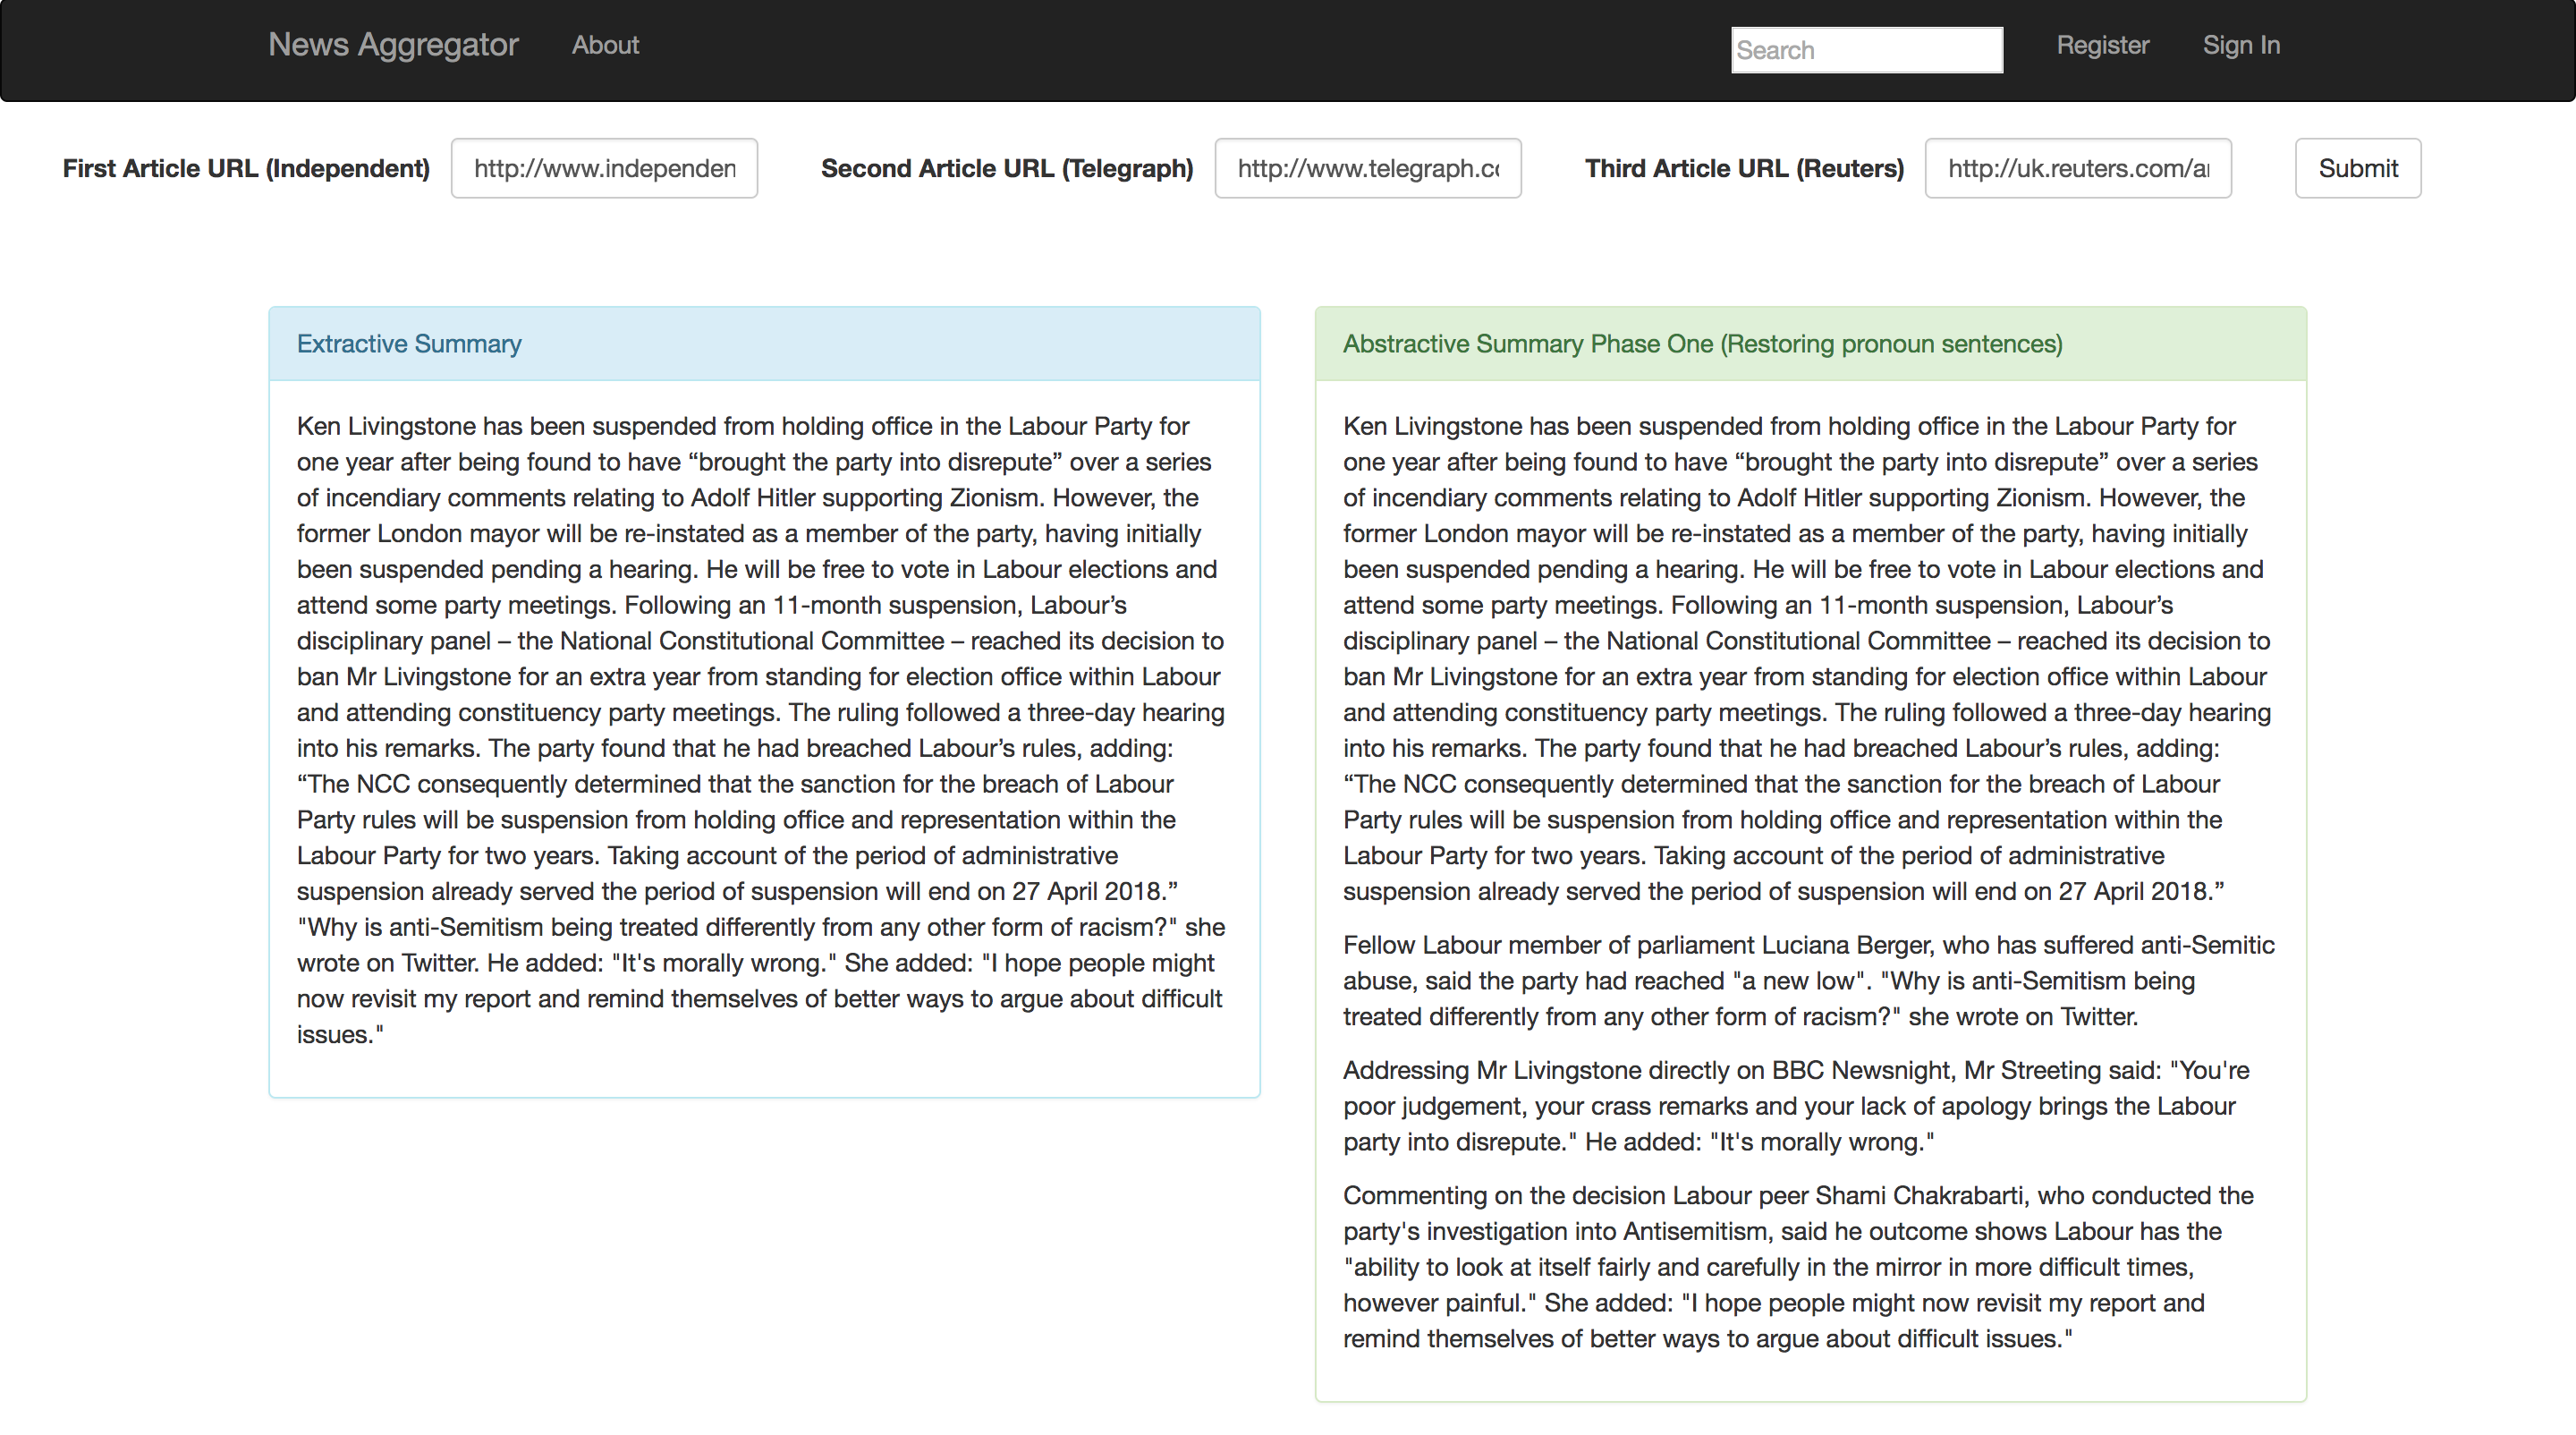
\includegraphics[scale=0.3]{SummaryEvaluationResource}
   \caption[A screenshot of the Summary Evaluation Resource]{A screenshot of the Summary Evaluation Resource. On the left is the extractive summary, and on the right is the extractive summary after the coreferences and quotations have been resolved as in Section \ref{extractiveimplementation}.}
   \label{summaryevaluationresource}
\end{figure} 

\subsubsection{An attempt at Abstractive Summarisation}

\label{abstractiveimplementation}

I made an initial attempt at abstractive summarisation, before reluctantly abandoning it on the grounds of infeasibility (further details on why are provided on why this was the case are given further on in this Section). \\

\textbf{Brief overview of Abstractive Summarisation algorithm}

The following algorithm presents in more detail the ideas presented in the Semantic Graph Section in Section \ref{abstractiveSummarisation}. \\

\begin{enumerate}
	\item \textbf{Rich Semantic Graph creation} \\ 
	In this process, the first step is to perform an analysis on each of the original articles using the Stanford CoreNLP \cite{corenlp} library. I then perform coreference resolution on the articles, replacing relevant nodes in the summary. I do this because it reduces the length of the summary significantly. The Rich Semantic Graph is then created from the Rich Semantic Subgraphs, which are created according to the procedure below. 
	\item \textbf{Rich Semantic SubGraph creation} \\
	In this step, the original summary is converted into several rich semantic subgraphs. First, the Stanford analyses computed in the first step are used to find a collection of "Relation Triples". Relation Triples are groups of subject, verb, object patterns. Each of these triples will be given its own subgraph. Each word in the triple is fed into the WordNet library \cite{wordnet} (Section \ref{WordNet} to find all the possible meanings of the word. \\
	Once every possible meaning has been found, the cartesian product of every possible meaning is generated, and assigned a score based off the WordNet usage statistics. The graph is created from this cartesian product, with each meaning of an individual word constituting a node. 
	\item \textbf{Rich Semantic Graph reduction} \\
	The graph is reduced by applying heuristics to combine sentences. For example, if two consecutive sentences both have the same subject, they can be combined into one sentence, with a conjunction for the object. 
	\item \textbf{Natural Language Generation}\\
	The final stage is to pass the reduced semantic graph into a natural language generator, in order to generate the final summary sentences.\\
\end{enumerate}

\textbf{Feasibility issues}

The major issue with this algorithm again centred around time. The designer of the algorithm had only presented results on simple sentence structures. As a result, when it came to the more complex structures and sentence lengths that inevitably appear in news articles, the algorithm began to struggle.

The major issue came in the creation of rich semantic subgraphs. Take the following relation triple for example.\\

\begin{displayquote}\emph{
Computing is hard\\}
\end{displayquote}

According to WordNet, there are two meanings to the word "computing", eleven for the word "is" and twelve for the word "hard". All told, that alone would result in 264 different combinations presented in the cartesian product. Given this would be just one out of potentially dozens of relation triples in an article, the amount of time to generate a single summary would become prohibitive. As a result, I decided that it would make more sense to focus on making the extractive summarisation as readable as possible instead. 

\subsection{Restlet}

\label{Restlet}

For my server I used the Restlet \cite{restlet} framework for Java. Restlet is a powerful open source framework that allows users to create vastly scalable Rest APIs and back end servers. There are three key classes in Restlet that I used.\\

\begin{itemize}
	\item \textbf{ServerResource} is a wrapper class, that provides the class with both a request object, and a response object. A server method can be created by using the annotation @Get or @Post as appropriate above a method. 
	\item \textbf{Application} is the base class for Restlet. Here, in an overrided method createInboundRoot I set the routes for the API to follow, and which ServerResource subclass to use when a request comes in to a specific api address. 
	\item \textbf{TaskService} is a service that allows the asynchronous scheduling and running of "tasks". I used this to run the server jobs required for fetching, labelling, clustering and summarisation. 
\end{itemize}

Documentation on the Web API I created is provided in Appendix \ref{WebAPI} and for the server jobs in Section \ref{ServerTasks}.

\subsection{Server Tasks}

\label{ServerTasks}

The following jobs are back end server tasks using the Restlet \cite{restlet} framework's TaskService (Section \ref{Restlet}). I created them with the purpose of fetching, labelling, clustering and summarising articles. They also perform other important tasks such as sending digests to subscribed users.  

\subsubsection{Scheduling of tasks}

\begin{figure}[ht!]
  \centering
    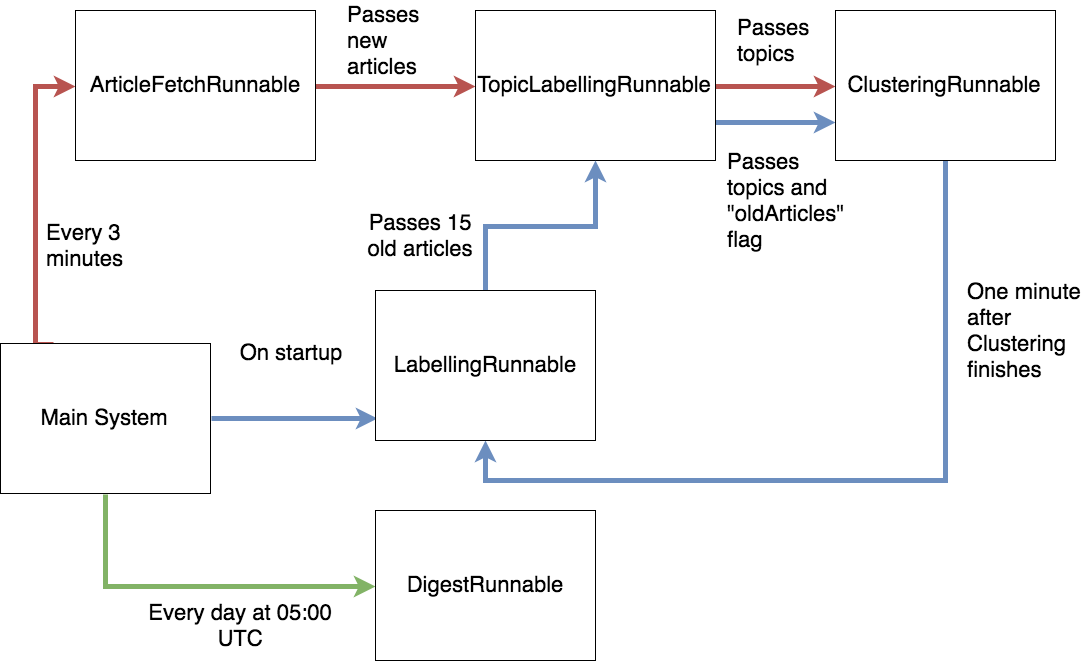
\includegraphics[width=\textwidth]{TaskService.png}
   \caption[A diagram showing the scheduling of tasks]{A diagram showing the scheduling of tasks using the TaskService and the flow of information in the server tasks.}
   \label{servertasks}
\end{figure} 

In order to make sure no new articles from external outlets are missed, the ArticleFetchRunnable is run every three minutes. The ArticleFetchRunnable, on completion, fires the TopicLabellingRunnable with the new articles as a parameter (this only happens if there is at least one new article). Once the TopicLabellingRunnable has completed, it in turn fires the ClusteringRunnable. 

\begin{sloppypar}
The principle behind this is to create a cascading effect. With the ArticleFetchRunnable being called so frequently, the TopicLabellingRunnable should rarely have to deal with a large batch of articles in a single run (the largest recorded so far is 22 articles in one Runnable). This cascading effect also means that the ClusteringRunnable wouldn't have to deal with a massive batch of topics at any one time either. This will all minimise the delay between an article first being published on an external outlet, and then reaching the NewSumm website.
\end{sloppypar}

With the LabellingRunnable, once the articles that have been picked up have gone through the whole process, and clustering has finished, the ClusteringRunnable then schedules the LabellingRunnable to start again a minute later. This means that only a maximum of one thread in the thread pool is dedicated to summarising old articles, and as many threads as possible can be dedicated to bringing news to the website as soon as possible after publication.

The DigestRunnable is fired once a day, at five in the morning in the UTC time zone.

Figure \ref{servertasks} shows how tasks are scheduled in the back end, and how the information flows between the separate server tasks.

\subsubsection{ArticleFetchRunnable}

The ArticleFetchRunnable runs through every source and fetches the latest articles. Each article is then checked against the database to see if it exists. If it does, then it is removed from the list of latest articles, whereas it is kept if it isn't present in the database.

Each article has the "isLabelled" flag set to false, and is then saved to the database.

\subsubsection{TopicLabellingRunnable}

The concept of the TopicLabellingRunnable is to model and label a set of articles. It has a constructor that takes as a parameter a list of articles. 

The Runnable models and labels each article, changing the "isLabelled" flag on the articles to true, and the "NeedsClustering" flag on the labels to true, before saving all to the database. 

\subsubsection{ClusteringRunnable}

The ClusteringRunnable is responsible for both clustering topics, and for producing the summaries. 

Initially, each label is clustered. Then, for each cluster, a "power set", consisting of all possible combinations of articles in the cluster (of size greater than or equal to one) is created. For each combination of articles an extractive summary is produced (this allows for the customisation of survey sources). 

Once the summaries have been generated, the clusters have been saved. They are added to the list of the labels' clusters in the database. In addition to this, for each label, a call to the Wikipedia API is made to find the list of categories that the label belongs to. The clusters are added to these labels as well.

In a time-saving measure, a list of clusters that have been summarised during the course of the runnable is kept. This means that if a cluster is created that has already been created for a different label, it doesn't need to be summarised again.

The "NeedsClustering" on the labels are also set to false.

\subsubsection{LabellingRunnable}

The LabellingRunnable's main function is to find articles that, for various reasons, could have "slipped through the cracks". It is fired at regular intervals, and takes fifteen articles from the database that have been marked as needing labelling, and calls the TopicLabellingRunnable with these articles.

\subsubsection{DigestRunnable}

The DigestRunnable is run each day. It goes through each user in the database, creating digests for those who have requested them. It then saves these digests in the database, thus creating an ID that is used to create a link to each. It then sends an email to each of the users with a digest, each email equipped with the generated link to view their digest.

\subsection{Front End}

\label{frontendimplementation}

For the implementation of the front end, I created a website and an iOS app.

The iPad version of the iOS app is designed to mirror the interface of the desktop website, whilst the iPhone version mirrors the interface of the mobile website. 

There are a few key differences from the initial design. These are:

\begin{itemize}
	\item \textbf{Article Viewer} - This screen now allows a greater amount of customisation on a user's part. Each article that the summary is created from is now accompanied by a switch. Turning this switch off will remove the article from the summary. The same happens in the opposite direction.
	\item \textbf{Summary Annotations} - Users can now see where the individual sentences of their summary are coming from. There is now a checkbox marked "Show Summary Annotations" in the corner, and when selected the text from the summary is highlighted according to its source (the source colours are shown on the corresponding switches on the right of the screen). Clicking on a highlighted piece of text will reveal a popover showing the source, along with the original sentence. If a sentence has some related sentences that aren't in the summary, the text won't be highlighted, and the popover will show the original, as well as all related sentences. \\
\end{itemize}

Screenshots from the website and apps can be seen in Figure \ref{appscreenshots}, and further details are provided in the user guide in Appendix \ref{userguide}.

\begin{figure}[ht!]
  \centering
  \begin{subfigure}[t]{0.6\textwidth}
        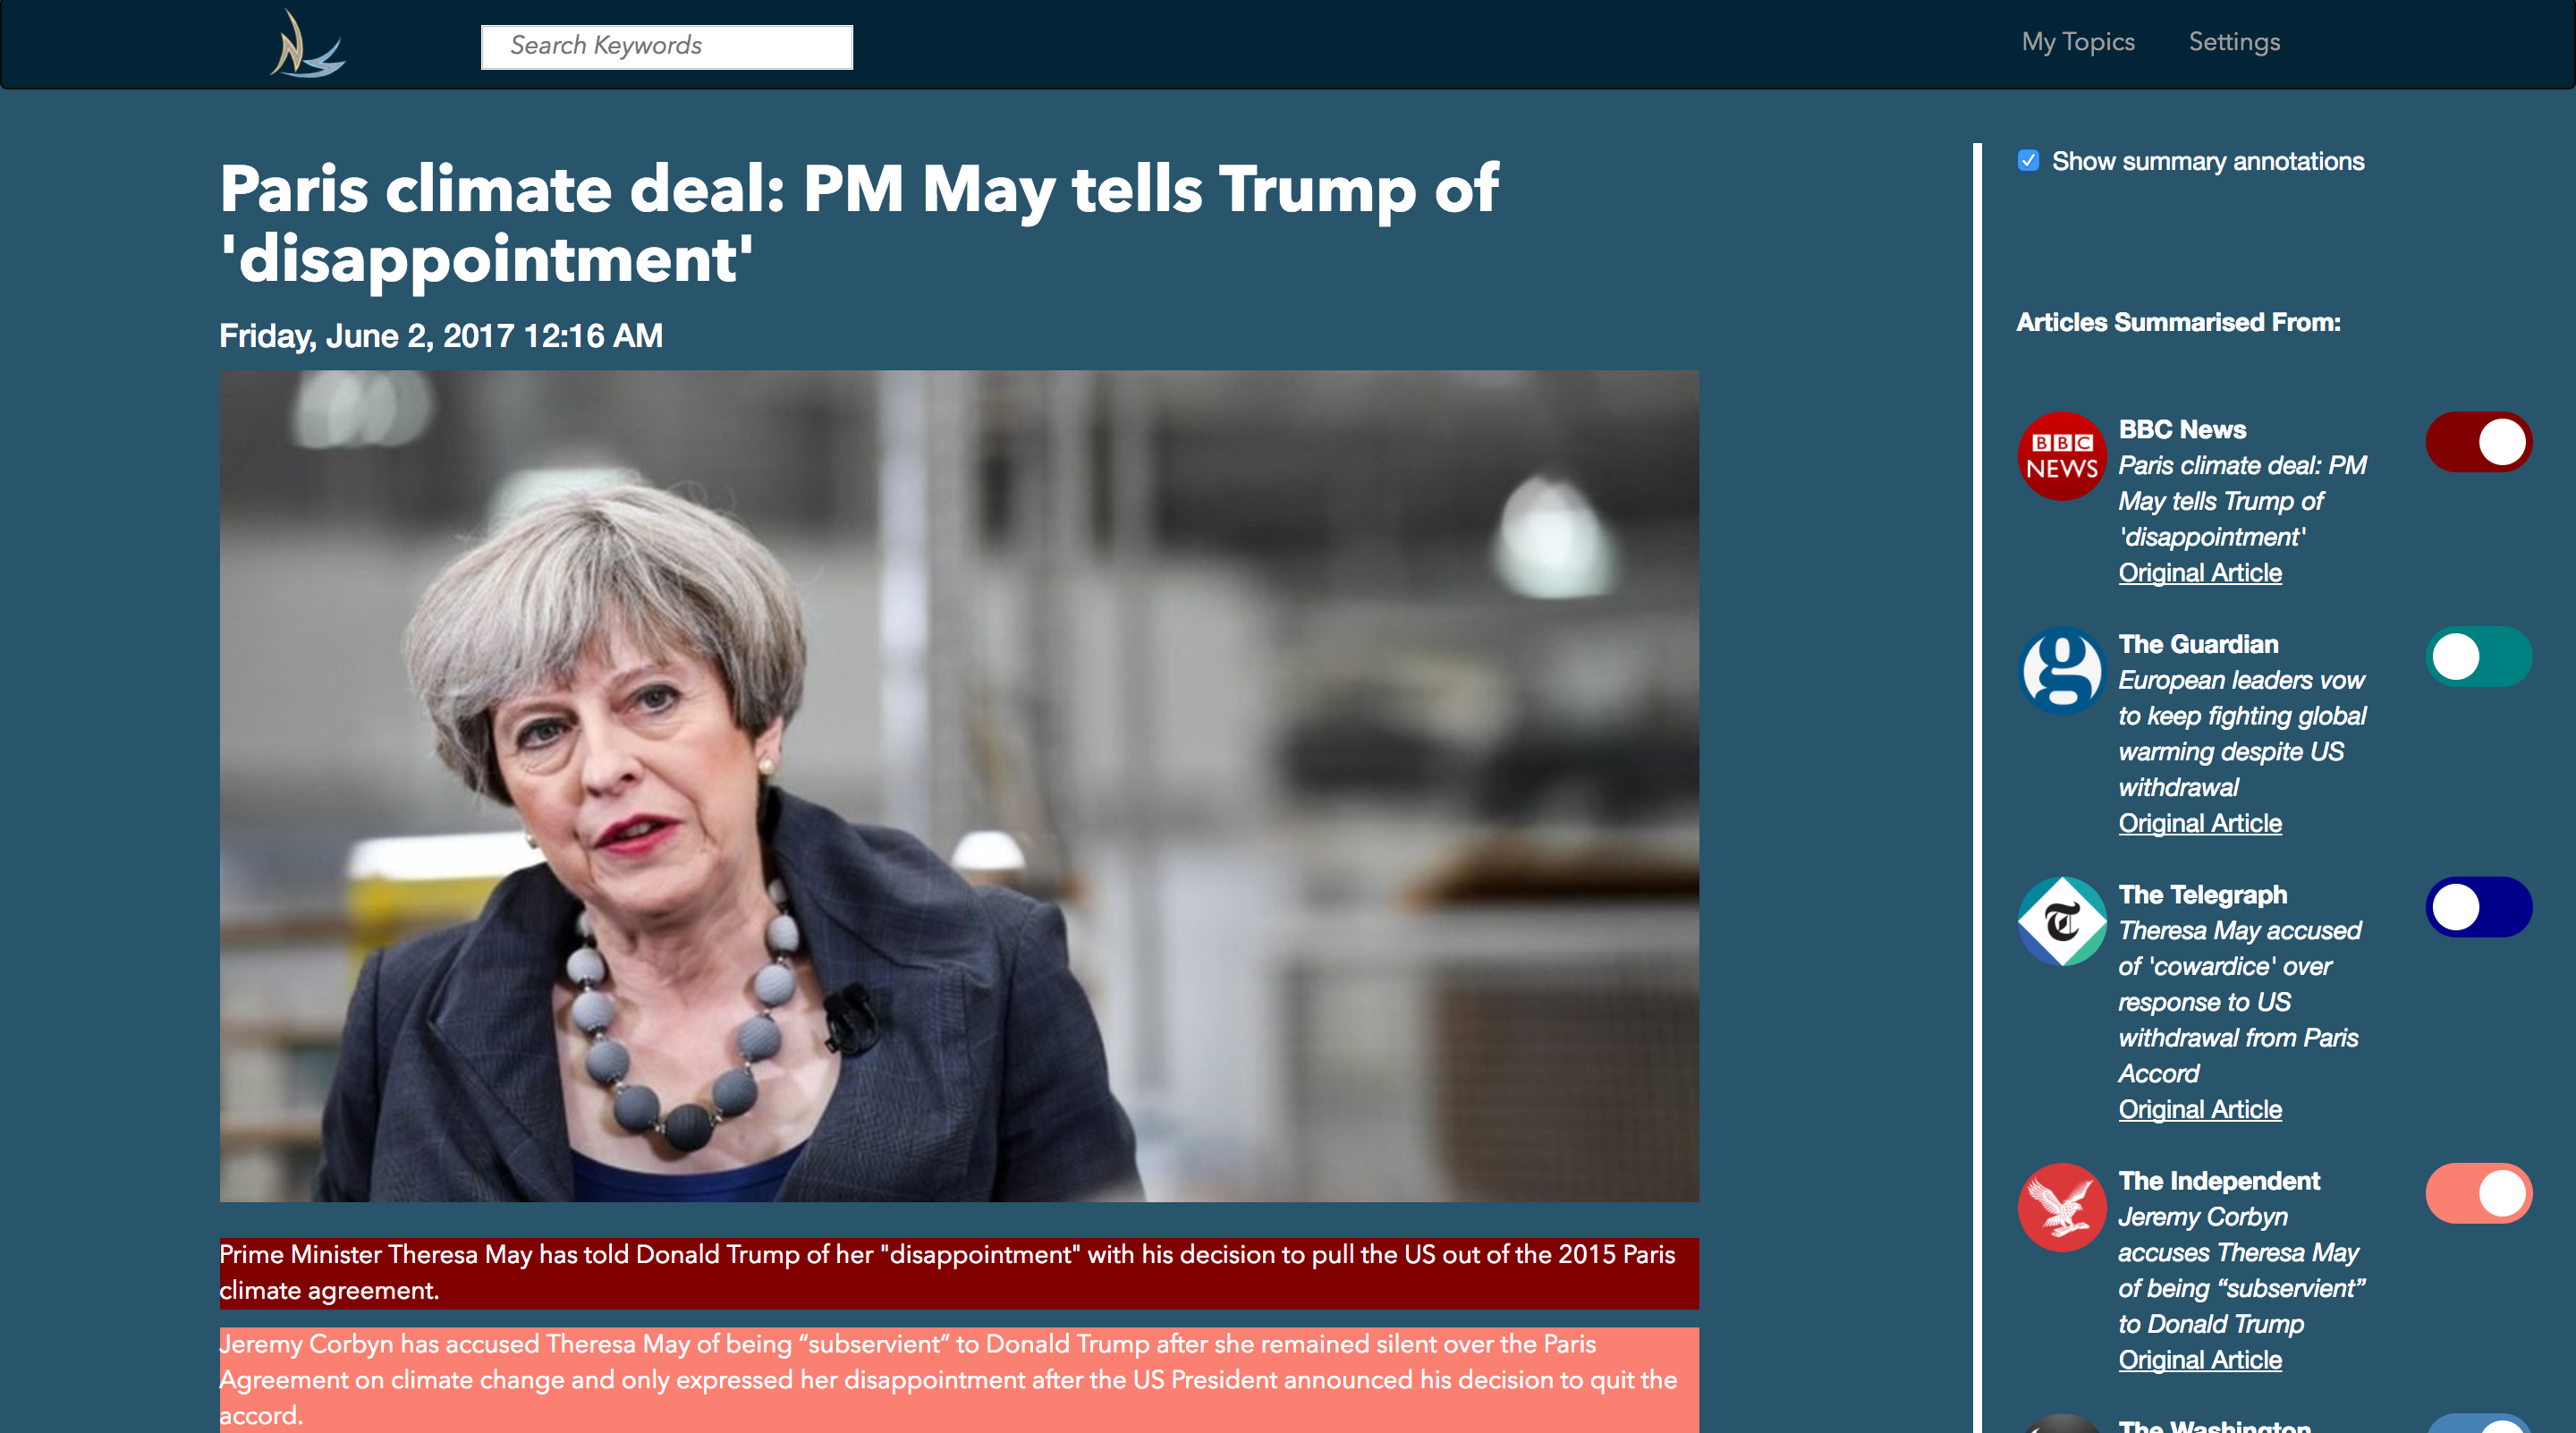
\includegraphics[width=\textwidth]{DesktopScreenshot}
        \caption{The article viewer, with summary annotations on, on the desktop website.}
    \end{subfigure}
   \qquad
    \begin{subfigure}[t]{0.3\textwidth}
    
\includegraphics[width=\textwidth]{iPhoneScreenshot.PNG}
   \caption{Search Results on the iPhone application.}
   \end{subfigure}
   \qquad
    \begin{subfigure}[t]{0.6\textwidth}
    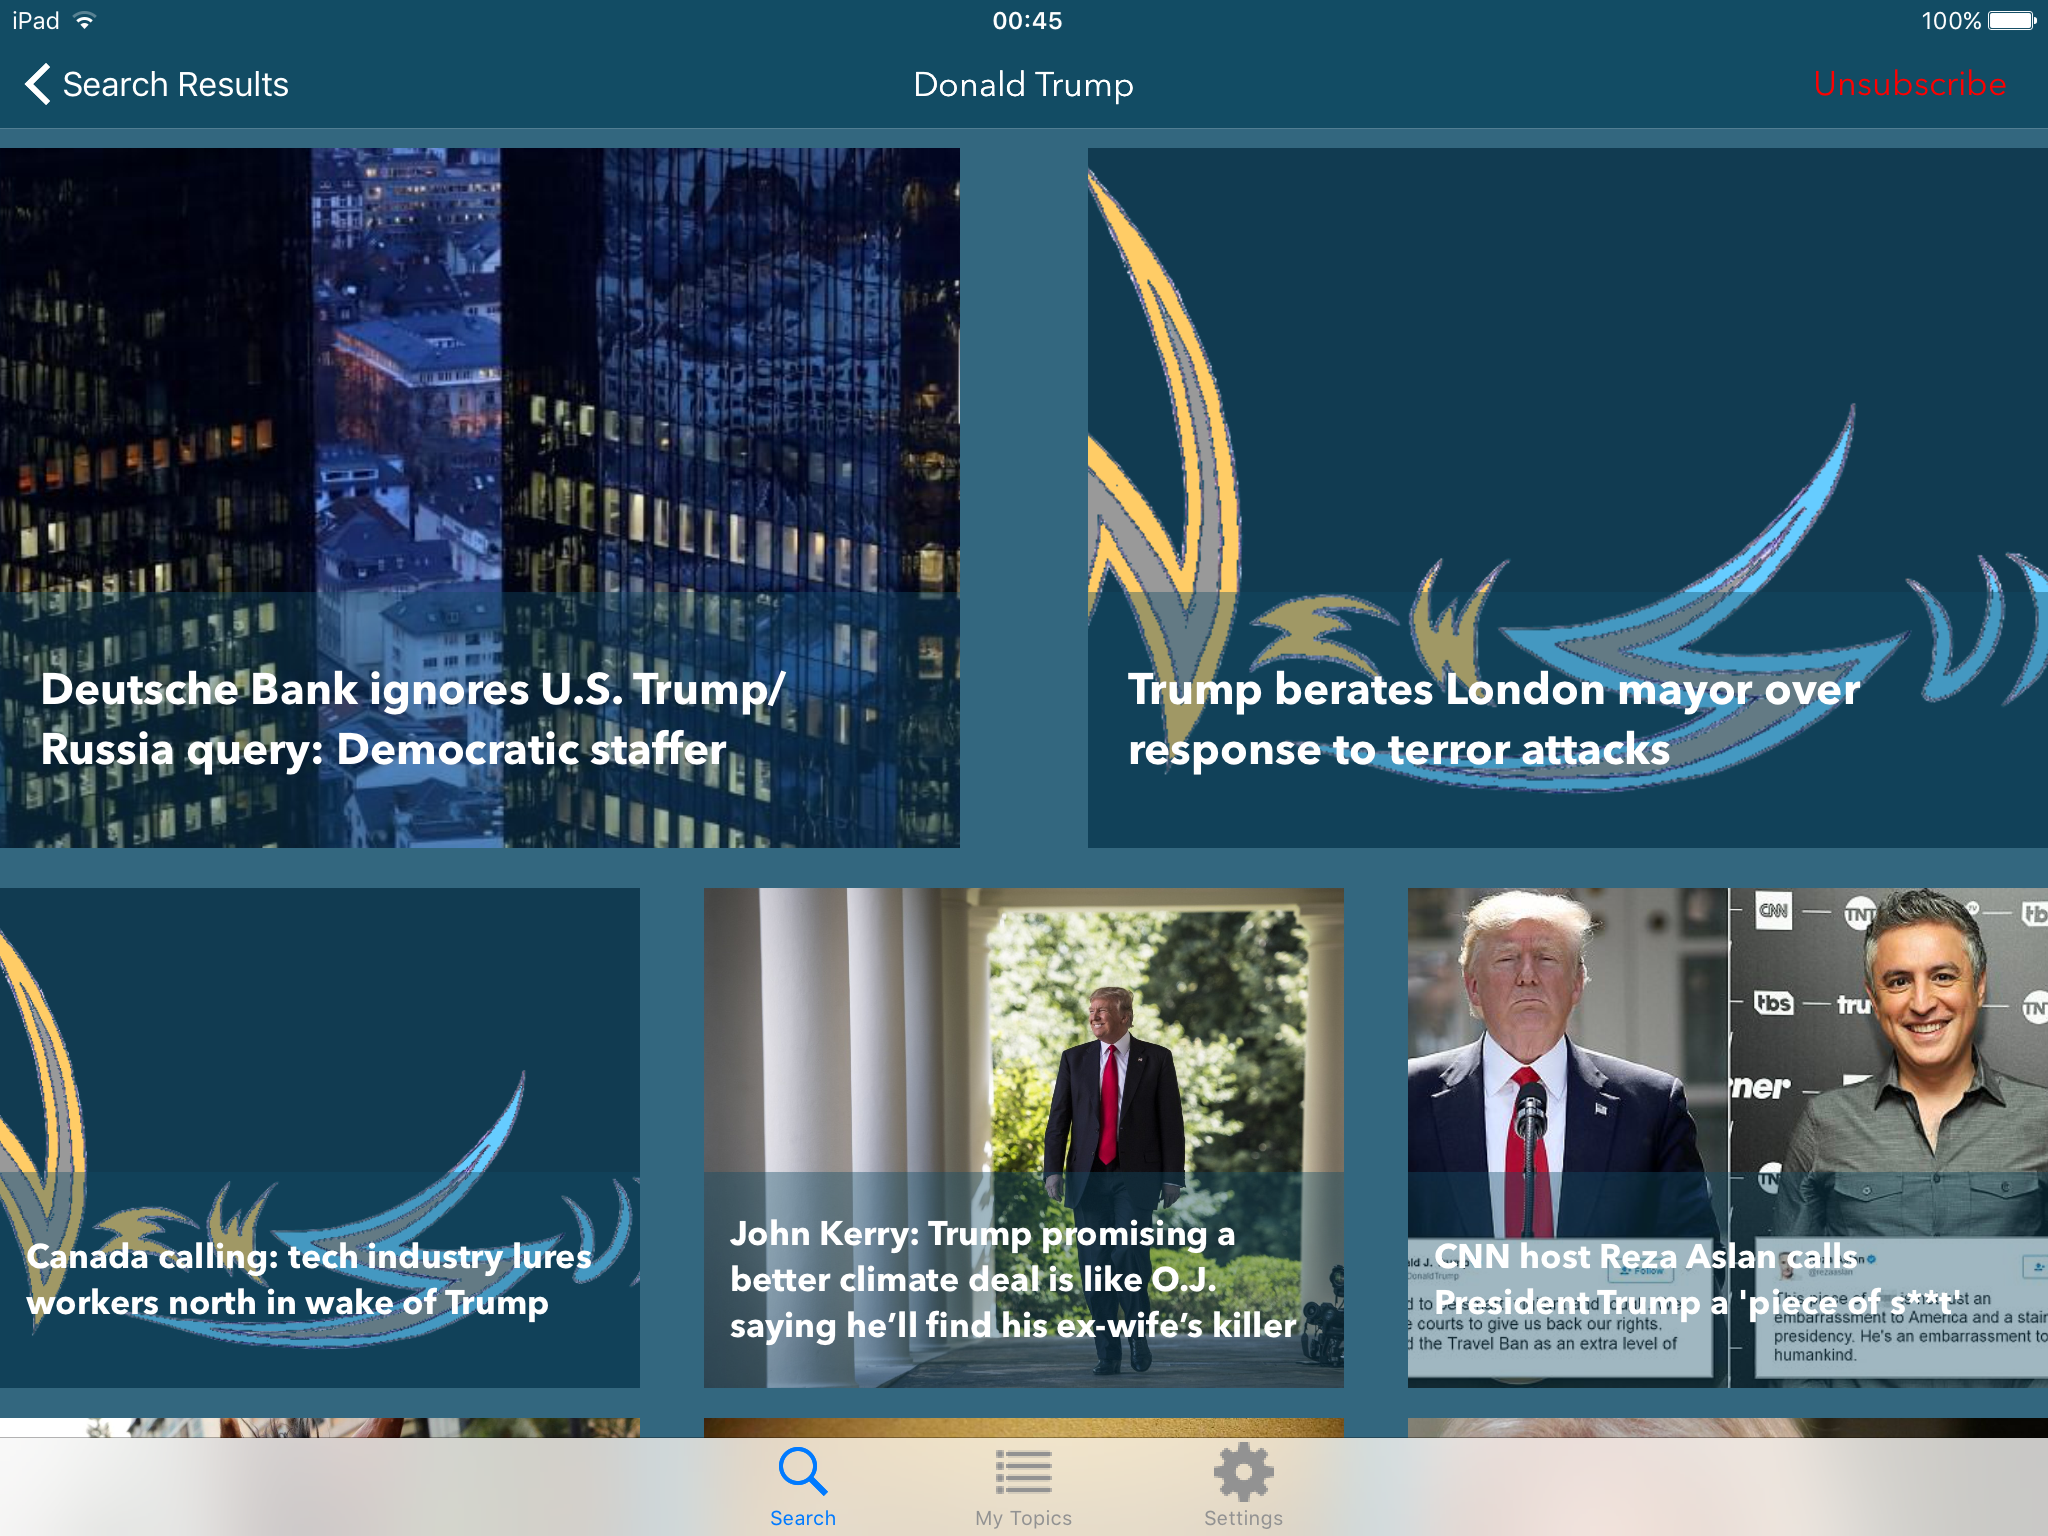
\includegraphics[width=\textwidth]{iPadScreenshot.PNG}
   \caption{The topic viewer on the iPad application.}
   \end{subfigure}
   \caption[Screenshots from the website and iOS Applications]{Screenshots from the website and iOS Applications.}
   \label{appscreenshots}
\end{figure}

%%%%%%%%%%%%%%%%%%%%%%%%%%%%%%%%%%%%%%%%%%%%%%%%%%%%%%%%%%%%%%%%%%%%%%%%%%%%%%%%%%%%%%%%%

\clearpage

\section{Evaluation}

The process of evaluating the project is three-fold. The first part was focused on evaluating the three key areas of the back end flow: Topic Labelling, Clustering and Summarisation. To do this, I sent out a survey on social media that presented the respondents with articles that have been labelled, articles that have been clustered, and articles that have been summarised (Section \ref{mlsurvey}). They were asked to rate each labelling, clustering and summarisation out of ten. This survey was then used to determine what parameters worked better for each phase of the back end. 

The second phase was evaluating the user interface. To do this, I sent out a second survey on social media (Section \ref{uisurvey}). This survey took potential users through the WebApp on a variety of devices (ranging from a standard desktop to tablets to mobile phones), asking them to perform basic tasks. At set stages of this survey, it also asked users to rate certain screens from one to ten, and to provide suggestions as to how these could be made more user-friendly. In addition to this I performed demonstrations of the WebApp and iOS applications at an Undergraduate Fair. Here I distributed a more simple Feedback Form, that requested feedback from attendees, and suggestions of what could be improved (Section \ref{uifeedback}). Finally, I also distributed the iOS application to a group of beta testers, made up of prospective users who had expressed an interest in the project at various stages, to get their opinions and suggestions.

Finally, I performed an in-depth analysis of the summariser itself, in an attempt to identify any major weaknesses in the tool. 

\subsection{Machine Learning and Summarisation Survey}

\label{mlsurvey}

The following survey was conducted using SurveyMonkey \cite{surveymonkey}, and was answered by 26 respondents. A link to the original survey can be found in Appendix \ref{mls}. The survey was split into three key sections: Labelling, Clustering and Summarisation. 

\subsubsection{Labelling}

To evaluate the labelling section, I selected at random three articles from the database and presented them to the respondents, along with the corresponding labels that the algorithm produced. Whilst chosen randomly, each article had been labelled using different parameters, and so the results would help determine which set of parameters is the most appropriate for the labelling algorithm.

The respondents were requested to score each labelling out of ten, and to suggest labels that should (or should not) have been on the list. \\

\textbf{First article}

\begin{mdframed}

\emph{Conservative social care funding cap: Theresa May defends changes} \cite{tmarticle}

Theresa May has defended her changes to the Tory social care policy, as critics called it a "manifesto meltdown".

The PM told the BBC "nothing has changed" and said rival parties had been "trying to scare" elderly people.

It came after she said earlier that there would be a cap on how much people paid for care - a change from the original policy which included no cap.

She did not say what level the cap would be set at but said it would be in a post-election consultation.

Labour and the Lib Dems said the Conservative social care policy was "in meltdown".

Since the publication of the Conservative manifesto last week, much attention has been focused on reforms to the way care for elderly and vulnerable adults is funded.

The manifesto did not mention an overall cap on costs, instead proposing a \pounds100,000 "floor" beyond which people's assets would be protected.

Speaking to activists in Wales earlier, Mrs May said the package would now include an "absolute limit" on the money people would have to pay - triggering accusations that she had made a U-turn.

In her interview, with the BBC's Andrew Neil, Mrs May denied this and said the principle the policy was based on remained absolutely the same.

The whole package will be put out to consultation, Mrs May said, adding that people had been "worried" by the Labour Party saying her reforms could mean they would have to sell their homes to pay for care.

Including an overall cap would mean the Tories were "protecting people for the future," Mrs May said.

"We are providing a system that provides sustainability in our social care for the future and we have got an ageing population. We need to do this otherwise our system will collapse."

Since the manifesto launch on Thursday, ministers had been saying the idea of a cap - as proposed by a government review in 2011 - had been rejected. \\

\end{mdframed}

\begin{mdframed}

\emph{Labels:}

"May", "Theresa May", "May Queen", "Elizabeth May", "Jeremy Corbyn", "United Kingdom general election, 2015", "Forms of government", "Labour", "Elderly care", "Self-care", "Primary care", "May ministry", "Nick Clegg", "Conservatism", "Wales", "United Kingdom general election, 2005", "United Kingdom general election, 2010", "United Kingdom general election, 1997", "Thursday", "Health", "Investors in People", "Jeremy Hunt", "BBC", "Labour Party", "Yesterday", "Last Week Tonight with John Oliver", "2011", "Andrew Neil", "Scottish Parliament election, 2016", "Day care", "Managed care", "Home care", "Transitional care", "Neonatal intensive care unit" \\

\end{mdframed}

\emph{Results:}

As Figure \ref{label1} shows, this labelling received an average score of 7.31 out of 10. I considered this score to be strong, as it indicated a general satisfaction. Comments afterwards on the survey indicated that the obstacle to the labelling receiving a higher score was the level of false positives included. The labelling had included the heuristic of finding labels by sourcing proper nouns in the original article. However, this included finding dates, money, and percentages, which resulted in false positives such as "Yesterday", "2011" and "Last Week Tonight with John Oliver", which are clearly not relevant to the article.

\begin{figure}[ht!]
  \centering
    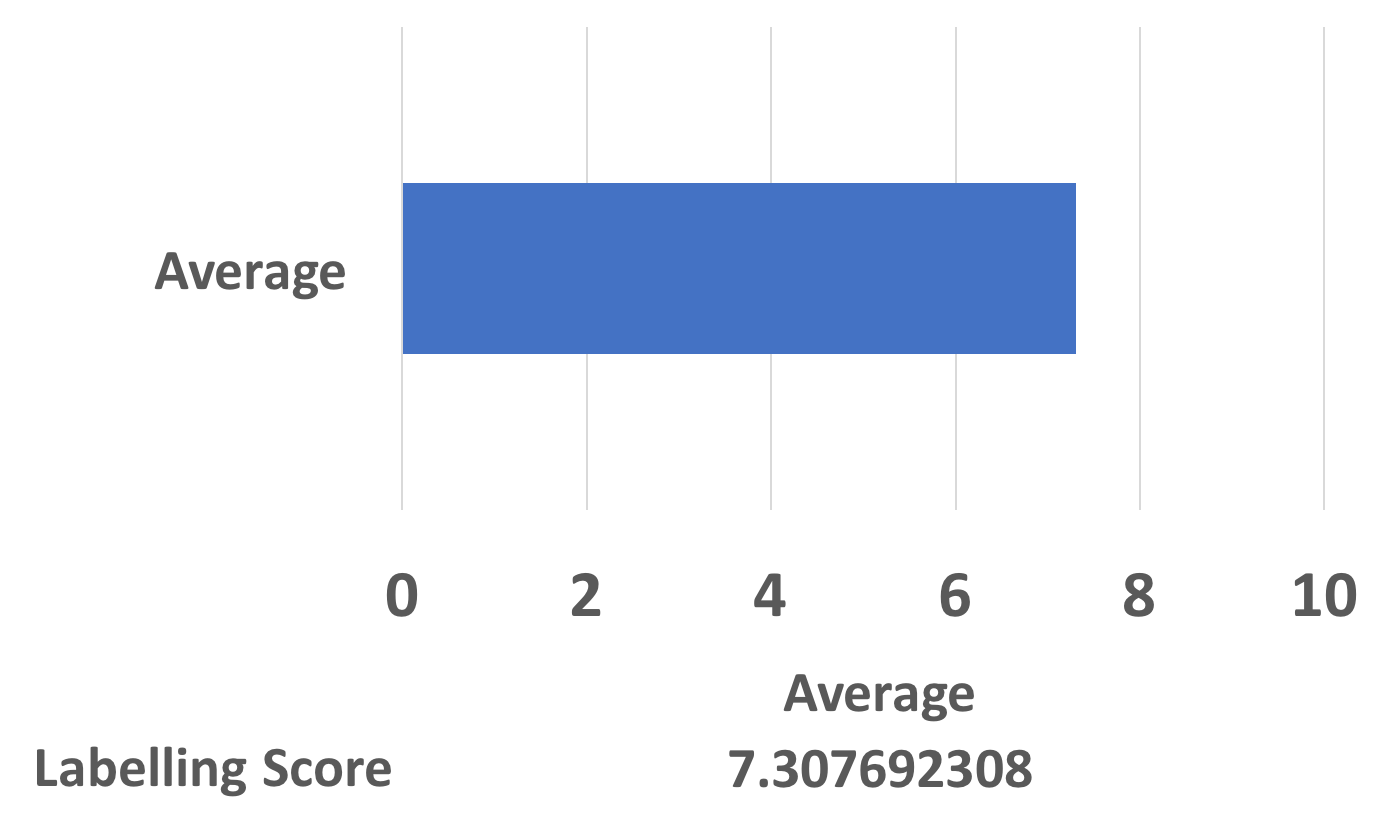
\includegraphics[scale=0.6]{label1score.png}
   \caption[The average score for a labelling]{The average score for the first article's labelling.}
   \label{label1}
\end{figure} 


\textbf{\\ Second Article}

\begin{mdframed}

\emph{Chelsea flower show: "abandoned Maltese quarry" wins top prize} \cite{cfsarticle}

It was not supposed to be pretty, but the judges certainly found it impressive. James Basson's take on an abandoned Maltese limestone quarry has won best in show at this year's Chelsea flower show.

The construction, which includes slabs of limestone and evergreens, perennials and ground cover, was designed to show the interaction between humans and nature on the island, Basson has said, and draws attention to the balance that needs to be maintained.
 
"I am absolutely thrilled to have won best in show for the first time," Basson said on Tuesday. "It is an incredible feeling and a testimony to the hard work of the whole team."

He thanked his wife, Helen, as well as Crocus, the nursery that built the garden, and his financial backer, M\&G Investments, for the roles they played.

"The garden is faultless and outstanding in terms of both construction and attention to detail," said the chair of the judging panel, James Alexander-Sinclair, after the decision was announced.

Discussing his design beforehand, Basson stressed its ecological message. After a research trip to the Maltese quarry that the garden is intended to evoke, he told the Daily Telegraph that it was "not supposed to be pretty. It is stark and monumentally brutal."

"I am fanatical about quarries anyway; the cleanliness and purity of them can be like a contemporary building. I love the graphic patterns of the blocks, the scouring marks, and the way nature regenerates after man has left. A client told me about this one, and when I had the chance of coming to Malta for a design job, I came to see it and was blown away," he said.

His design was divided into zones, each with its own ecology. It included shrubland, the landscape of the hills of the Mediterranean coastline and clifftop scenes, echoing the variety seen in Malta.

The garden also received the best construction award - the second such award in two years for Crocus.

"The message behind the designer's creation is that humans need to take action to preserve the fragile environment of our planet. Sustainable water disposal, recycling and composting: all are vital if Malta is to save its distinct and delicate landscapes," said the Royal Horticultural Society, which runs the annual flower show in London.

It said it awarded 73 gold medals. Kate Gould's "city living" garden, representing an urban apartment block and how to innovatively use space in an urban context, won best fresh garden. The award for best artisan garden went to Walker's wharf garden, supported by Doncaster Deaf Trust, by the designer Graham Bodle. \\

\end{mdframed}

\begin{mdframed}

\emph{Labels:}

"Chelsea", "The Daily Show", "Mediterranean Sea", "Helen", "Canada", "London", "The Tonight Show with Jay Leno", "Malta", "Tuesday", "The Oprah Winfrey Show", "May 23", "Chelsea Handler", "Peep show", "The Tonight Show Starring Johnny Carson", "Northern Ontario", "Royal Horticultural Society", "Wouter Basson", "James Basson", "James Sinclair (footballer)", "You're invited to Mary-Kate and Ashley's (film series)", "Party lists in the New Zealand general election, 2002", "The House Always Wins", "Football in Malta", "Quarry", "Maltese people", "Italian Maltese", "Maltese language", "Maltese (dog)", "Languages of Malta", "Maltese", "Callow Rock quarry", "Broadcroft Quarry"  \\

\end{mdframed}

\emph{Results:}

As Figure \ref{label2} shows, this labelling received an average score of 4.39 out of 10. I was expecting this article to receive a lower score out of ten, as it was an early iteration of the parameters used. In this case the number of labels to return had been artificially increased - my reasoning for this at the time was that this would increase the chances of slightly more obscure (but relevant labels) would be found in this way. However, users felt that this meant that the quality of labelling overall significantly deteriorated, as the level of false positives was far higher than the first article.

\begin{figure}[ht!]
  \centering
    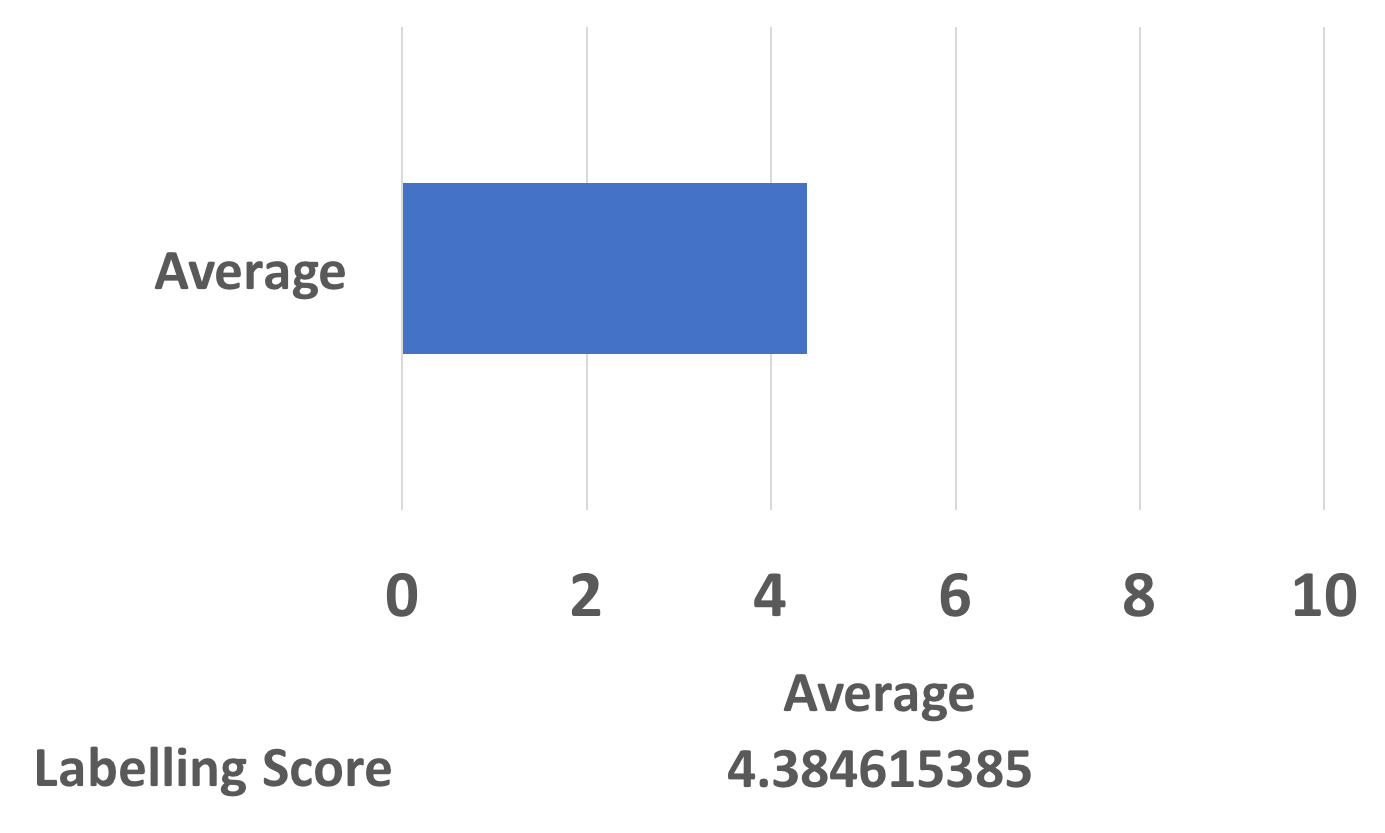
\includegraphics[scale=0.6]{label2score.png}
   \caption[The average score for a labelling]{The average score for the second article's labelling.}
   \label{label2}
\end{figure} 

\textbf{\\ Third Article}

\begin{mdframed}

\emph{Global markets are fighting back against Trump uncertainty} \cite{trumparticle}

After a brutal beatdown on Wednesday, investors are wasting no time picking themselves up off the mat. The S\&P 500 climbed 0.6\% to 2,370.71 at 2:24 p.m. ET, close to its highest level of the day. It's been quite the recovery for the benchmark. In premarket trading, the index looked headed for a second straight drop following former FBI Director Robert Mueller's appointment as special counsel to investigate Russian efforts to influence the November election. All it took was some better-than-expected economic data for them to change their tune, as initial jobless claims unexpectedly dropped. The relief rally can also be seen elsewhere in global markets. Haven assets gave back some earlier gains as gold decreased by 1\% and the yen slid by 0.7\% versus the US dollar. But the relief did not translate overseas, as the Stoxx Europe 600 dropped by 0.5\% during regular trading hours, while the MSCI All-World Index lost 1.2\%. The relatively muted reaction is a far cry from what was seen Wednesday, when the S\&P 500 dropped 1.7\%, its biggest decline since September 9, and a stock market fear gauge spiked by almost 50\%. The snappy recovery in stocks should be of little surprise, considering US equity investors have made a habit of buying on weakness throughout the eight-year bull market. Following the UK's vote last June to leave the European Union, the S\&P 500 fell by 5.3\% over two trading sessions, only to make up those losses in about a week. The same dynamic was in play when China unexpectedly devalued its currency in August 2015. After the S\&P 500 underwent an 11\% correction, traders bought the dip and restored the benchmark to its pre-sell-off levels within about two months. \\

\end{mdframed}

\begin{mdframed}

\emph{Labels:}

"Time zone", "Time in China", "Pacific Time Zone", "Market (economics)", "Capital market", "Emerging markets", "Prediction market", "Fish market", "Donald Trump", "Day", "Robert Mueller", "Haven" \\

\end{mdframed}

\emph{Results:}

As Figure \ref{label3} shows, this labelling received an average score of 6.54 out of 10. This score was better than I expected. The labelling used a version of the algorithm that didn't make use of the name finder, so as to increase the speed of labelling. As a result, the number of labels returned are far lower. Whilst users felt that again the labels weren't largely relevant, they scored this set of labels higher than for the second article because there were fewer false positives than before (because there were simply fewer labels).

\begin{figure}[ht!]
  \centering
    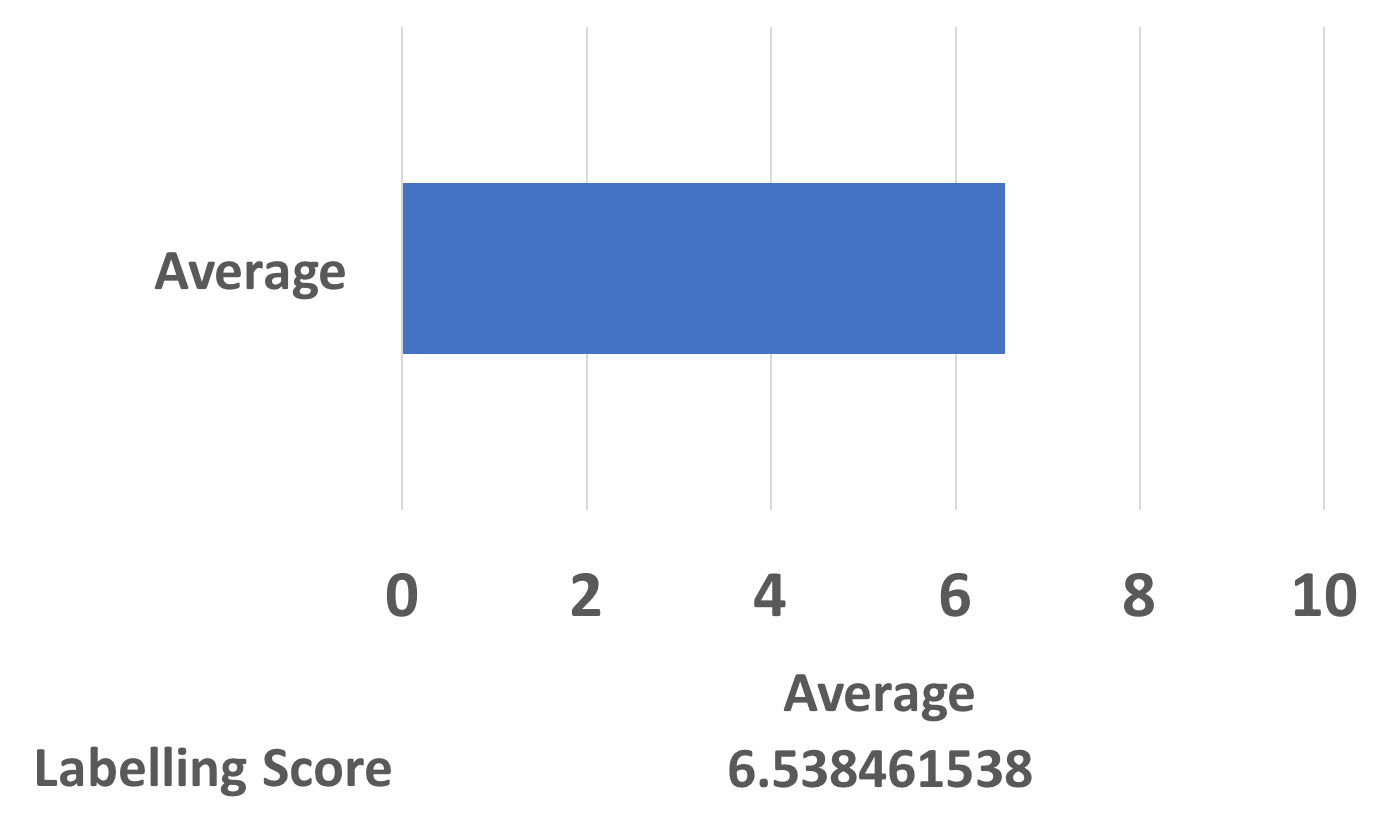
\includegraphics[scale=0.6]{label3score.png}
   \caption[The average score for a labelling]{The average score for the third article's labelling.}
   \label{label3}
\end{figure} 

\textbf{\\ Labelling Conclusions}

The overarching criticism that people wrote about in the feedback section of the survey was that the labelling algorithm suffers from an issue of "false positives" - that is to say, it frequently identifies labels that in all likelihood shouldn't be present.

Key differences between the three articles is that the first one was labelled using an algorithm that used the Apache OpenNLP \cite{opennlp} library's name finder to find key words. In the second, the labelling algorithm was designed to return more results by default, which explains its low score (primarily because there were too many false positives, as well as the fact that it missed key names, such as "Chelsea Flower Show"). The third article used no name finder, and had a smaller number of labels to return.

In the final product, I chose to use the first labelling algorithm, but with a modified name finder, that would only return names for organisations, people and locations, as opposed to including dates, percentages and money. I did this because I determined from the difference in score between the first and third articles that use of the name finder justified the increase in time required to label an article. However, because of the false positives due to dates, percentages and money in the first article, I removed searching for these from the name finder. 

\subsubsection{Clustering}

For Clustering, I provided respondents with four different sets of articles that have been clustered. For each article I provided the headline and a link to the original article. As before, I asked respondents to rate each clustering out of ten and provide additional justification. The clusters below were randomly selected, based on criteria including number of articles in the cluster, and different parameters used to cluster. In my opinion, clustering requires better scores than labelling, as an incorrect cluster would automatically render a summary near useless. As a result, I decided that whilst a score of seven out of ten was strong for labelling, the bar would need to be closer to nine out of ten for clustering.\\

\textbf{First Cluster}

\begin{mdframed}

\emph{Cluster:}

Joe Biden just made a stunning admission about Hillary Clinton's 2016 election bid \cite{bidenarticle}

Congressman for Salem brilliantly trolls Donald Trump over "witch hunt" claims \cite{trumpsalem} \\

\end{mdframed}

\emph{Results:}

As Figure \ref{cluster1} shows, this cluster received an average score of 5.23 out of 10. This was largely expected, and in fact perhaps a bit higher than anticipated. The articles are about two different pieces of news, and shouldn't have been clustered together, hence the low score. This clustering algorithm used rather low thresholds for similarity, hence causing this false clustering.  \\

\begin{figure}[ht!]
  \centering
    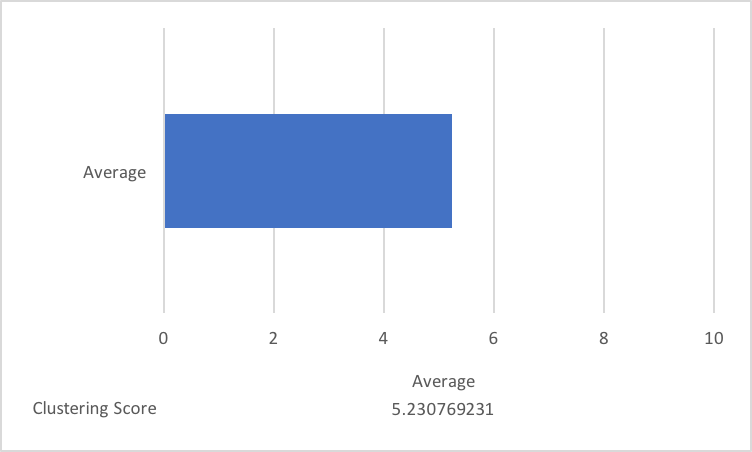
\includegraphics[scale=0.6]{cluster1score.png}
   \caption[The average score for a cluster]{The average score for the first set's clustering.}
   \label{cluster1}
\end{figure} 

\textbf{Second Cluster}

\begin{mdframed}

\emph{Cluster:}

Manchester United Player's Player of the Year revealed \cite{united1}

Manchester United Player of the Year awards are underway \cite{united2}

Live Manchester United Player of the Year Awards \cite{united3}

Our 7 favourite photos from Manchester United's Player of the Year Awards night \cite{united4}

Man United fans say the same thing as Ander Herrera is named Player of the Year \cite{united5}

Manchester United stars and WAGS turn on the style at Player of the Year awards \cite{united6}

Anthony Martial among five first-team absentees from Man Utd awards ceremony \cite{united7} \\

\end{mdframed}

\emph{Results:}

As Figure \ref{cluster2} shows, this cluster received an average score of 9.38 out of 10. This was very much expected, as the articles were within an hour of each other and ostensibly about the same piece of news. It represents an example that should be bread and butter for the clustering algorithm , and it passed with flying colours. \\

\begin{figure}[ht!]
  \centering
    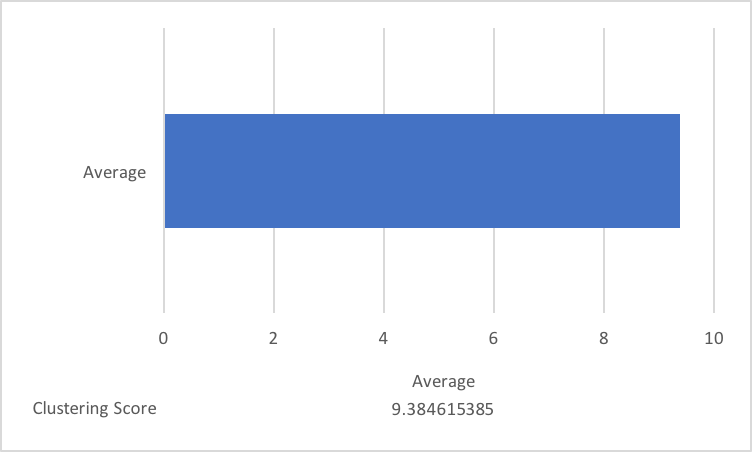
\includegraphics[scale=0.6]{cluster2score.png}
   \caption[The average score for a cluster]{The average score for the second set's clustering.} 
   \label{cluster2}
\end{figure} 

\textbf{Third Cluster}

\begin{mdframed}

\emph{Cluster:}

Uber to appeal arbitration ruling in self driving car lawsuit \cite{uber1}

Uber threatens to fire self-driving car engineer in trade secrets case \cite{uber2}

Uber threatened to fire engineer accused by rival Alphabet of stealing self-driving trade secrets \cite{uber3}

Uber is threatening to fire the engineer at the heart of its legal battle with Google \cite{uber4}

Uber threatens to fire former Google engineer over self-driving car spat with Waymo \cite{uber5} \\

\end{mdframed}

\emph{Results:}

As Figure \ref{cluster3} shows, this cluster received an average score of 6.54 out of 10. This cluster doesn't penalise the timestamp, and so an article that was published nearly a week before the others was included in the cluster, hence the lower score. Whilst this was largely expected, it did emphasise the fact that clustering had to be strong - the titles in this cluster were very similar, and yet the respondents noticed the difference between the articles in large numbers. \\

\begin{figure}[ht!]
  \centering
    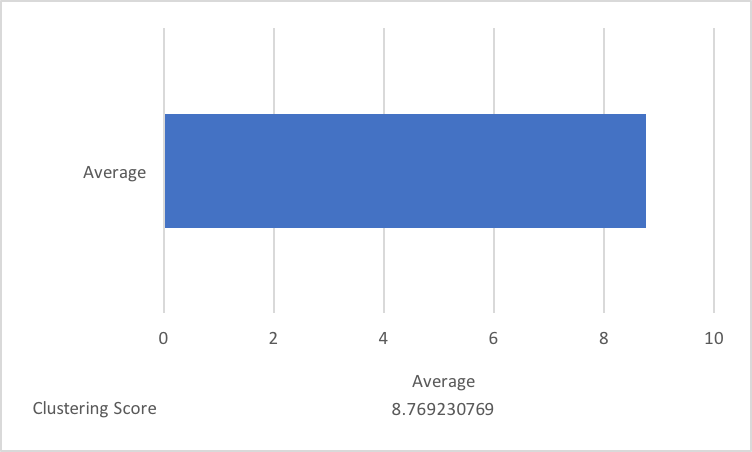
\includegraphics[scale=0.6]{cluster3score.png}
   \caption[The average score for a cluster]{The average score for the third set's clustering.}
   \label{cluster3}
\end{figure} 

\textbf{Fourth Cluster}

\begin{mdframed}

\emph{Cluster:}

"Two explosions" heard at Ariana Grande concert in Manchester \cite{ag1}

Concert goers "run out screaming" after loud bangs at Manchester Arena \cite{ag2}

Celebs pray for victims of Manchester Arena explosions \cite{ag3}

"A major incident targeted at our city" MPs respond to Manchester explosion \cite{ag4}

Emmerdale star Isabel Hodgins' horrifying Manchester Arena experience \cite{ag5} \\

\end{mdframed}

\emph{Results:}

As Figure \ref{cluster4} shows, this cluster received an average score of 9.23 out of 10. This, whilst indicating a very strong cluster, was ever so slightly below my expectations. I felt that this was a better cluster than the second cluster above. For this cluster I used the thresholds from the second cluster, along with an increased timestamp penalty when compared to the third article, hence the expectation of the high score. \\

\begin{figure}[ht!]
  \centering
    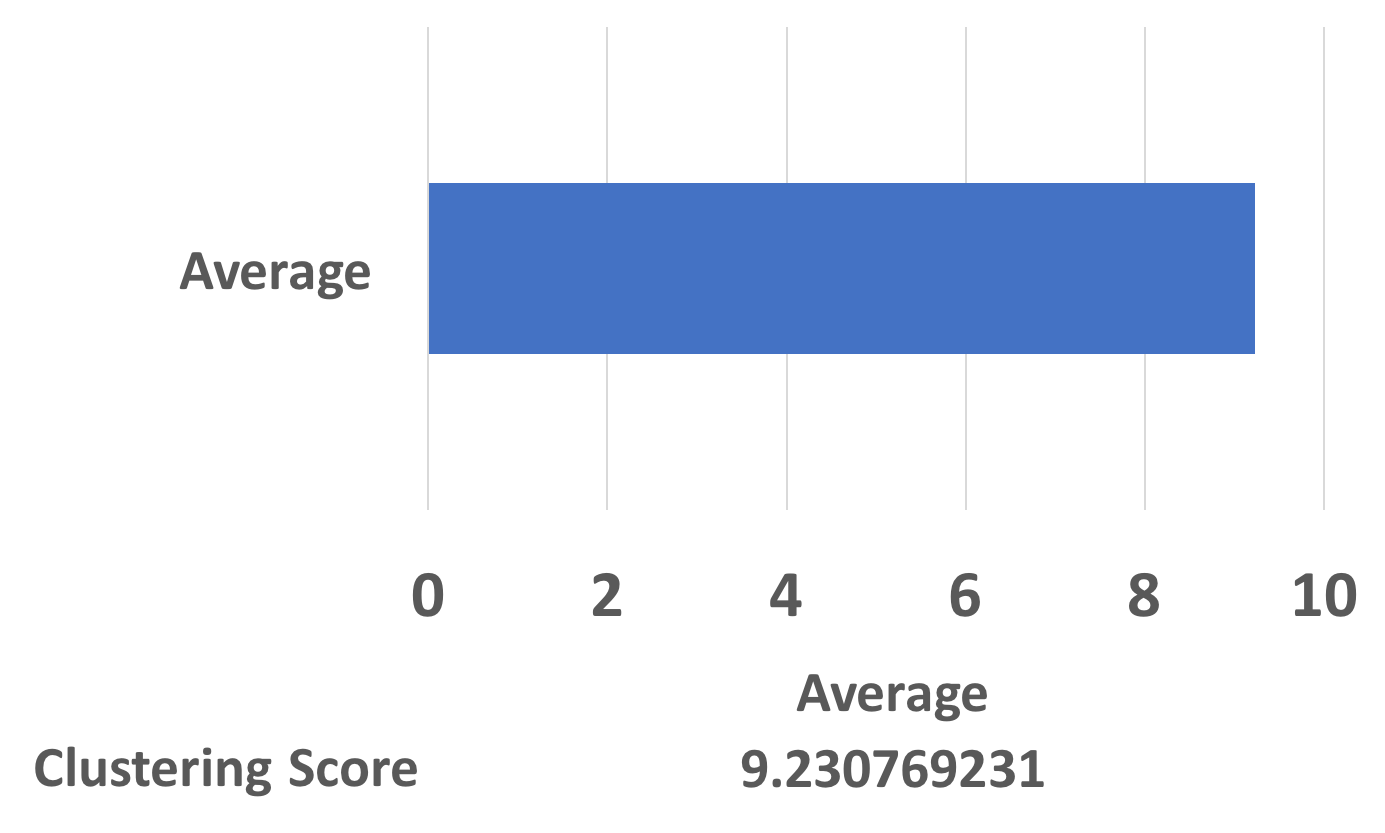
\includegraphics[scale=0.6]{cluster4score.png}
   \caption[The average score for a cluster]{The average score for the fourth set's clustering.}
   \label{cluster4}
\end{figure} 

\textbf{Clustering Conclusions}

In the first cluster, the main criticism was that the articles were about two very different topics. In reaction to this, I raised the thresholds significantly in the similarity algorithm. 

Whilst the second was universally agreeable, the third cluster had a lower score. This was because one of the articles in the cluster was about a slightly different topic, and had been published nearly a week before. In reaction to this, I increased the penalty for the difference in timestamps in the clustering algorithm, thus ensuring articles a week apart wouldn't be clustered together.

The final cluster was also considered to be very good, and incorporated the successful thresholds from the second cluster with a timestamp penalty derived from the third cluster. I used the thresholds and timestamp penalty from this cluster as the basis for the parameters of the clustering algorithm. I used these ahead of the second cluster's parameters as it had a higher penalty for the timestamp than for the second cluster, which was shown by the third cluster to be of major importance.

\subsubsection{Summarisation}

I presented respondents with summaries for three different clusters. The clusters were again chosen randomly, and users were again asked to give a rating for each out of ten and a justification for doing so. There is an argument for using the same clusters as before, but I didn't do this. I decided that it was more important to show users summaries for clusters that I knew were strong, so that they could view summaries for correct clusters. I decided that the key is for the summaries to be coherent and readable, and to have as few redundant sentences as possible. \\

\textbf{First Summary}

\begin{mdframed}

\emph{Cluster:}

"Two explosions" heard at Ariana Grande concert in Manchester \cite{ag1}

Concert goers "run out screaming" after loud bangs at Manchester Arena \cite{ag2}

Celebs pray for victims of Manchester Arena explosions \cite{ag3}

"A major incident targeted at our city" MPs respond to Manchester explosion \cite{ag4}

Emmerdale star Isabel Hodgins' horrifying Manchester Arena experience \cite{ag5} \\

\emph{Summary:}

Celebrities have begun paying tribute to victims of terrifying explosions inside Manchester Arena on Monday night.

Several people were killed after explosions were heard inside the venue, with video footage showing concert goers fleeing the arena after bangs rang out immediately after the Ariana Grande concert finished.

In response to the tragic events various celebs tweeted condolences and prayers.

Demi Lovato tweeted: "Tearing up imaging innocent concert goers losing their lives.. praying for everyone and all \#arianators."

Katy Perry responded on the micro blogging site: "Praying for everyone at @arianagrande's show".

While Ellie Goulding responded with a message to all affected by the tragic events: "Sending love to those affected in Manchester." Olly Murs wrote in two tweets.

"Shocked! Can't believe it!! Sending my love to everyone that was @ManchesterArena tonight!" and added, "No one should go to a concert and never come home".

Gary Lineker wrote: "Truly awful news from the great city of Manchester. Thoughts are with all those affected."

Jeremy Corbyn made sure to thank Emergency responders: "Terrible incident in Manchester. My thoughts are with all those affected and our brilliant emergency services."

Rio Ferdinand tweeted: "Just heard the news what's happening in Manchester.. hope everyone safe and sound!" Bloodied concertgoers were pictured being helped by emergency services outside the gig and armed police were seen patrolling the arena.

Evie Brewster, who attended the concert, told MailOnline: "Ariana Grande had just finished her last song and left the stage when a huge explosion sounded. Suddenly everybody started screaming and running for the exit." \\

\end{mdframed}

\emph{Results:}

As Figure \ref{summ1} shows, this summary received an average score of 7.54 out of 10. This summary is coherent, and so I expected this to receive a decent mark, which it did. A complaint from users was that the extremely short paragraphs meant that the summary was not as readable as it could be, which is why the score for this summary is not higher. \\

\begin{figure}[ht!]
  \centering
    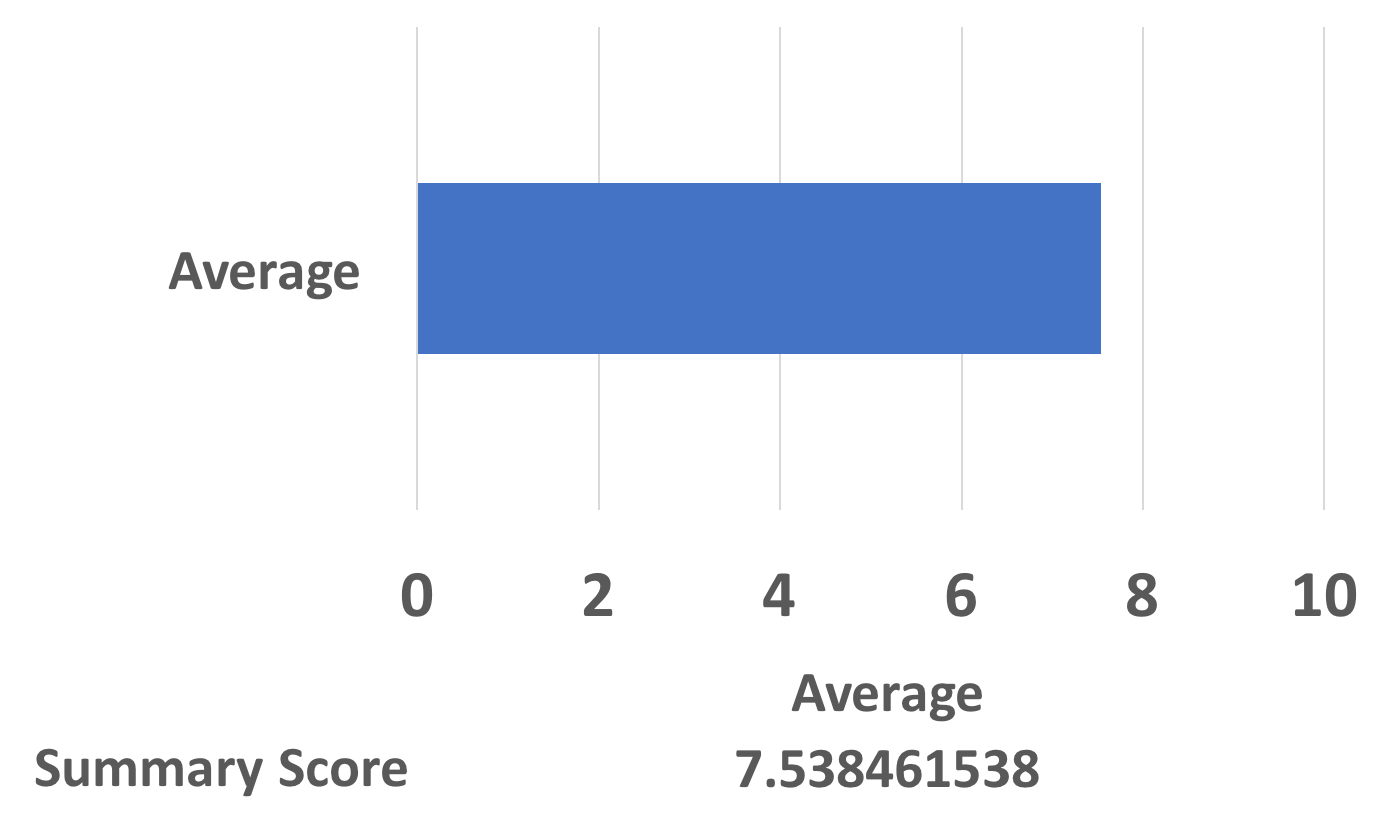
\includegraphics[scale=0.6]{summ1score.png}
   \caption[The average score for a summary]{The average score for the first cluster's summary.}
   \label{summ1}
\end{figure} 

\textbf{Second Summary}

\begin{mdframed}

\emph{Cluster:}

Donald Trump says special counsel "hurts our country" as Russia probe "becoming criminal investigation" \cite{trump1}

Trump says, speaking for himself, there was no collusion with Russia \cite{trump2}

Donald Trump says "even my enemies say there is no Russia collusion" \cite{trump3} \\

\emph{Summary:}

WASHINGTON President Donald Trump on Thursday said the appointment of a special counsel to investigate possible collusion between his presidential campaign on Russia was dividing the country, and he repeated his contention there was no such collusion.

Lindsey Graham, the Republican senator, said Russia probe seemed to be moving from counter-intelligence to a criminal investigation.

Mr Trump has told US media outlets that the appointment of a special counsel "hurts our country terribly" as it shows how divided the United States.

"I believe it hurts our country terribly, because it shows we're a divided, mixed-up, not-unified country," Mr Trump told news outlets.

He said the counsel was a "pure excuse for the Democrats having lost an election".

Michael Flynn discussed establishing a back channel for communication between Donald Trump and Vladimir Putin that could be used to bypass national security bureaucracy, it has been reported.

Mr Flynn and other advisers to the president's election campaign were in contact with Russian officials and others with Kremlin ties in at least 18 calls and emails during the last seven months of the 2016 presidential race, current and former US officials familiar with the exchanges told Reuters.

Mr Trump reacted angrily to the latest allegations on Thursday, tweeting: "With all the illegal acts that took place in the Clinton campaign \& Obama Administration, there was never a special coucel (SIC) appointed!"

Mr Trump added: "This is the single greatest witch hunt of a politician in American history!"

Describing the investigation into any possible links with Moscow, the President said he was the victim of a "witch hunt".

Six of the previously undisclosed contacts described to Reuters were phone calls between Sergei Kislyak, Russia's ambassador to the United States, and Trump advisers, including Mr Flynn, Mr Trump's first national security adviser, three current and former officials said.

Conversations between Mr Flynn and Mr Kislyak accelerated after the November 8 vote as the two discussed establishing a back channel for communication between Trump and Russian President Vladimir Putin that could bypass the US national security bureaucracy, which both sides considered hostile to improved relations, four current US officials said.

But the disclosure could increase the pressure on Mr Trump and his aides to provide the FBI and Congress with a full account of interactions with Russian officials and others with links to the Kremlin during and immediately after the 2016 election. \\

\end{mdframed}

\emph{Results:}

As Figure \ref{summ2} shows, this summary received an average score of 8.31 out of 10. A key difference between the first summary and this one is that the strategy for forming paragraphs is different. In this case, consecutive sentences from the same original source are grouped together, thus making longer, more coherent paragraphs. This is the key driver behind the higher score, as expected. \\

\begin{figure}[ht!]
  \centering
    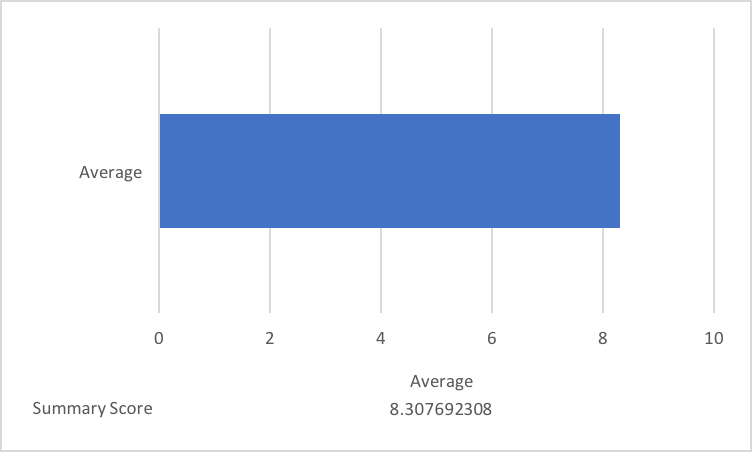
\includegraphics[scale=0.6]{summ2score.png}
   \caption[The average score for a summary]{The average score for the second cluster's summary.}
   \label{summ2}
\end{figure} 

\textbf{Third Summary}

\begin{mdframed}

\emph{Cluster:}

When is Pippa Middleton marrying James Matthews? Everything you need to know \cite{pippa1}

Pippa Middleton's dream wedding set to be soggy as Met Office predicts rain \cite{pippa2}

What time is Pippa Middleton's wedding and where is St Mark's Church? \cite{pippa3} \\

\emph{Summary:}

It is one element of a bride's big day that she has no control over: the weather.

So Pippa Middleton will be hoping that the forecasters are wrong to predict showers that threaten to hit during her wedding on Saturday.

The Duchess of Cambridge's younger sister is to tie the knot with James Matthews in what will be the society wedding of 2017.

Their ceremony is due to start at St Mark's Church in Englefield, Berkshire, at 11.30am on Saturday.

The Met Office is predicting rain for the area on Saturday - the same time Pippa and her new husband are likely to pose for wedding pictures.

But the couple will no doubt be hoping they can dodge the showers and enjoy some of the predicted sunshine that is likely to break through the clouds throughout the afternoon.

After making an unforgettable appearance at the royal wedding of big sister Kate, Pippa will take centre stage on Saturday at the picturesque 12th century church.

The Duke and Duchess of Cambridge will be among the guests as their children Prince George and Princess Charlotte play starring roles as a page boy and bridesmaid.

But Kate has already confessed to a Buckingham Palace garden party guest that she is a little apprehensive about how her children will behave.

Prince Harry will also be sitting among the congregation, but royal-watchers will be waiting to see if he brings his American actress girlfriend Meghan Markle.

Kate's controversial uncle, Gary Goldsmith, who was a guest at the Duke and Duchess of Cambridge's 2011 wedding, is also said to be attending.

Hedge fund boss Mr Matthews got down on bended knee during a trip to the Lake District last summer to propose to Miss Middleton.

At the time, the couple had been dating for less than a year, but had moved in together and a thrilled Pippa was said to have been totally surprised by the proposal. \\

\end{mdframed}

\emph{Results:}

As Figure \ref{summ3} shows, this summary received an average score of 8.85 out of 10. I expected this summary to score the highest out of the three, and it reflected in the final results. The summary is the most coherent and readable - in fact it almost reads like an actual article in its own right, as opposed to a summary of several articles. The higher score was because respondents felt that this summary had fewer redundant sentences, a direct result of a higher threshold when finding redundant sentences in the algorithm. \\

\begin{figure}[ht!]
  \centering
    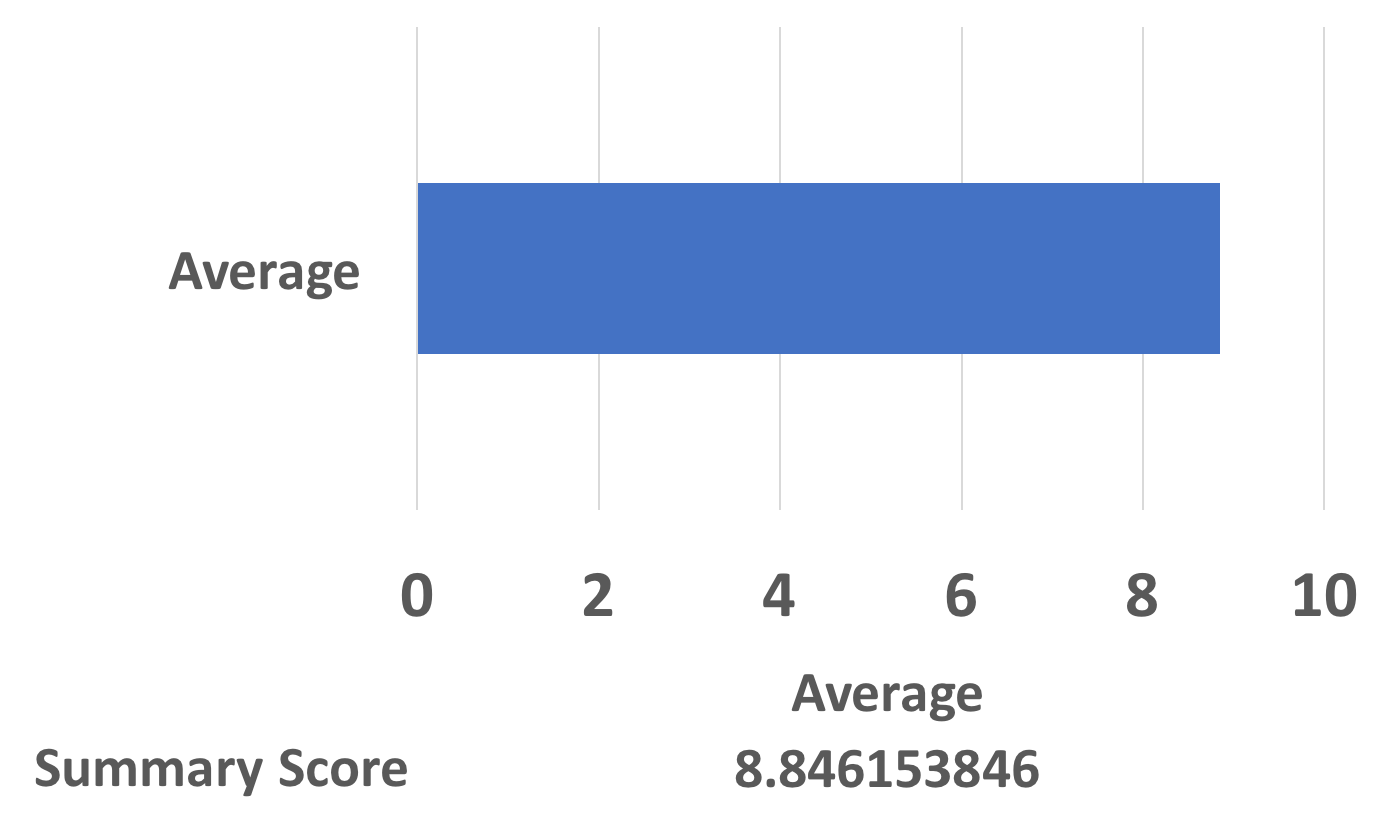
\includegraphics[scale=0.6]{summ3score.png}
   \caption[The average score for a summary]{The average score for the third cluster's summary.}
   \label{summ3}
\end{figure} 

\textbf{Summary Conclusions}

The reaction to the summaries was reasonably positive. In the first summary, a common criticism was that the way the paragraphs were breaking in the summary made it much less readable. 

The second and third summaries both used a different procedure for breaking paragraphs up, which was much better received. The second summary has a slightly lower score than the third summary as it was believed the second summary had a few more redundant sentences than the third. As a result, the threshold for redundant sentences in the summarisation algorithm was set at the level of the third summary.

\subsection{User Interface Evaluation}

The evaluation of the user interface was three-fold. First, I provided a survey that asked respondents to perform certain functions and provide their opinions on how easy or difficult certain features were to use. Then I went to an Undergraduate Fair, and provided a demonstration of the product to peers, asking them to fill out feedback forms afterwards. Finally, I distributed the iOS app to a group of testers to try out. 

\subsubsection{A Survey}

\label{uisurvey}

The following is a subset of the answers given to the survey (to which the link can be found in Appendix \ref{uis}), which was filled in by 22 respondents. These respondents were sourced using social media, and largely in the young to middle aged age bracket. They also all indicated in the first survey about News Reading Habits (Section \ref{survey}) that they would be interested in using a news summariser, making their opinions all the more important (which is why these respondents were sought after). A majority of questions in this survey asked the respondents to perform a task on the WebApp, before following up on whether it worked, and whether they found it easy to do. Answers to these questions are omitted below. The answers that are shown below are responses to questions about users' opinions of the various aspects of the WebApp in general, and their justifications for them. \\

\textbf{Search Results}

At this stage of the survey, a user has been asked to search for the topic "Russia" on the home page, and have now reached the search results screen.

The panels on the search results screen provide the first 250 characters of the Wikipedia \cite{wikipedia} article pertaining to the topic. However, users were split on whether this was clear or not (Figure \ref{ui1}), and in fact were generally in agreement that there needed to be more clarity on this (Figure \ref{ui2}). 

In order to tackle this issue, I added "Wikipedia:" in front of each 250 character extract. \\

\begin{figure}[ht!]
  \centering
    \includegraphics[scale=0.6]{ui1.png}
   \caption[A graph depicting responses to the User Interface Survey]{}
   \label{ui1}
\end{figure} 

\begin{figure}[ht!]
  \centering
    \includegraphics[scale=0.6]{ui2.png}
   \caption[A graph depicting responses to the User Interface Survey]{}
   \label{ui2}
\end{figure} 

\textbf{Topic Viewer}

Once the user has clicked on the "Russia" topic, they are taken to the Topic Viewer screen. Users generally felt very happy with the layout of this screen (Figure \ref{ui3}), but one point for improvement was that the screen was very "data hungry" and "took too long to load".

In reaction to this, I decided to streamline the information that is provided to the Topic Viewer screen through the API. Details on this can be found in the Optimisation section (Section \ref{apioptimisation}). \\

\begin{figure}[ht!]
  \centering
    \includegraphics[scale=0.6]{ui3.png}
   \caption[A graph depicting responses to the User Interface Survey]{}
   \label{ui3}
\end{figure} 

\textbf{Article Viewer}

At this point the respondent has been provided a link to a specific article. 

Users were happy with the layout of the article viewer (Figure \ref{ui4}), but felt that the image was a bit too large. This was rectified afterwards.

The users were then taken through the steps of using the Summary Annotations portion of the screen. Feedback for this was again positive, if a bit lower than the score for the article viewer overall (Figure \ref{ui5}). A lot of the reasoning for this was that the availability of certain features needed to be made clearer, which they have been in later versions of the product, with the help of status messages in the bottom right-hand corner of the screen. \\

\begin{figure}[ht!]
  \centering
    \includegraphics[scale=0.6]{ui4.png}
   \caption[A graph depicting responses to the User Interface Survey]{}
   \label{ui4}
\end{figure} 

\begin{figure}[ht!]
  \centering
    \includegraphics[scale=0.6]{ui5.png}
   \caption[A graph depicting responses to the User Interface Survey]{}
   \label{ui5}
\end{figure} 

\textbf{Topic Dashboard and Topic Settings}

The final aspects of the survey centre around the topic dashboard and the topic settings pages. The user first visits the topic dashboard, where they should see their subscription to the "Russia" topic that they searched for earlier. Users again felt positive about this screen (Figure \ref{ui6}).

One of the last tasks the respondents were asked to perform was the deselection of default sources for the "Russia" topic. Users felt that this was not intuitive (Figure \ref{ui7}) and that there should be some more information explicitly informing a user what deselecting a source does. This has since been put in.

\begin{figure}[ht!]
  \centering
    \includegraphics[scale=0.6]{ui6.png}
   \caption[A graph depicting responses to the User Interface Survey]{}
   \label{ui6}
\end{figure} 

\begin{figure}[ht!]
  \centering
    \includegraphics[scale=0.6]{ui7.png}
   \caption[A graph depicting responses to the User Interface Survey]{}
   \label{ui7}
\end{figure} 

\subsubsection{Feedback from Undergraduate Fair}

\label{uifeedback}

At the Undergraduate Fair twelve peers filled out the feedback form (Appendix \ref{uif}) for the product. The overarching theme of the feedback was that the product would be more than useful, as it would "save a lot of time" and "users won't need to read as much". This is a clear indication that NewSumm goes some way, if not all the way to solving the volume problem set out in the Introduction (Section \ref{intro}).

Users felt that the User Interface was very polished, but that the overall WebApp was at times frustratingly slow. This point, which also came up at points in the main survey, is addressed in Section \ref{apioptimisation}.

\subsubsection{iOS Applications}

Due to limitations imposed by Apple \cite{apple} on the distribution of applications, evaluation of the iOS app could not be performed in the formal manner that the Back End and WebApp had been evaluated. 

As a result, I assembled a group of "testers" who would sign up as a beta tester of the application on iTunes Connect \cite{itunesconnect}, allowing them to download a build of the app without it being formally placed on the App Store.

The last build of the iPhone application was installed 11 times, and the last build of the iPad application was installed 8 times. A total of four different builds were looked at by testers, with each new build being released in response to feedback from the previous.   

\subsection{Summary Analysis}

In this section I aimed to analyse the summaries that are produced by the back end. To do this, I used a Jupyter \cite{jupyter} notebook and python to analyse different aspects of each summary in the database. I then transferred the data into Microsoft Excel \cite{excel}, and made use of its extensive graphing capabilities to visualise the data.

\subsubsection{Outlet Matrix}

\begin{sidewaysfigure}
    \centering
    \includegraphics[width=\textwidth]{matrix.png}
    \caption{A matrix comparing outlets when summarised together}
    \label{fig:matrix}
\end{sidewaysfigure}

Figure \ref{fig:matrix} shows a matrix of different sources when pitted against each other. To produce this matrix, I took each of the outlets that are used in the back end. For each outlet, I then found the summaries it has in common with each of the other outlets. For the purposes of this matrix, I only included summaries where there were only these two outlets, thus enabling a direct comparison without external interference.

In each set of summaries I found how the text was split between the two outlets, and recorded the average percentages in the matrix. This matrix will be used in the following sections in order to identify interesting points in the data. 

The matrix is colour coded. The averages in the final column are on a colour scale, with the highest values being dark green, and the lowest being a deep red. On the inner columns of the table, a cell is coloured yellow if between 30 and 40, and 60 and 70. It is coloured red if below 30, green if above 70 and not shaded if between 40 and 60.

\subsubsection{Neutral Outlets}

Ignoring sources such as ESPN \cite{espn}, Cricinfo \cite{cricinfo} and Four-Four-Two \cite{fourfourtwo}, which are purely sporting websites, the two key "neutral" sources in the application are the BBC \cite{bbc} and Reuters \cite{reuters}.

Figures \ref{bbc-news} and \ref{reuters} paint a stark picture on summary distribution when these two sources are included. In fact, the matrix (Figure \ref{fig:matrix}) says that the BBC and Reuters have the two lowest contributions to summaries out of all the outlets in the system. 

For the BBC, the percentage contribution is below 50\% for the vast majority of other outlets, whilst the same can be said of Reuters.

Also notable from the charts is the fact that, with the exception of The Daily Mail \cite{dailymail} in the BBC's case and The Telegraph in Reuters', the neutral sources fare poorly against the partisan UK newspapers that are in the system (namely The Daily Mail, The Guardian \cite{guardian}, The Telegraph \cite{telegraph}, The Mirror \cite{mirror} and The Independent \cite{independent}). 

A explanation for this would be that the BBC and Reuters supply the facts for a summary, whilst the partisan organisations produce articles that are a bit more opinionated. These opinions are then prioritised by the LexRank algorithm \cite{lexRank} as they are usually unique, and so are included in droves, thus marginalising slightly the apparent contributions of the neutral sources. 

\begin{figure}[ht!]
  \centering
    \includegraphics[scale=0.15]{bbc-news.png}
   \caption[A graph depicting responses to the User Interface Survey]{The percentage of summaries that originates from the BBC \cite{bbc} when compared to other outlets.}
   \label{bbc-news}
\end{figure} 

\begin{figure}[ht!]
  \centering
    \includegraphics[scale=0.15]{reuters.png}
   \caption[A graph depicting responses to the User Interface Survey]{The percentage of summaries that originates from Reuters  \cite{reuters} when compared to other outlets.}
   \label{reuters}
\end{figure} 

\subsubsection{The Political Spectrum}

In February 2017 polling organisation YouGov \cite{yougov} ran a poll to find out the public's perception of the political leanings of mainstream newspapers in the United Kingdom \cite{yougovarticle}. Their results found that The Daily Mail \cite{dailymail} is viewed to be Britain's most right-wing paper, whilst The Guardian \cite{guardian} edges The Mirror \cite{mirror} as the most left-wing. The Independent \cite{independent} is considered broadly centrist, whilst The Telegraph \cite{telegraph} is also placed on the right (Figure \ref{yougov}). 

\begin{figure}[ht!]
  \centering
    \includegraphics[scale=0.4]{yougovpoll.png}
   \caption[A graph depicting responses to the User Interface Survey]{The results of the YouGov poll.}
   \label{yougov}
\end{figure}

NewSumm has five outlets that are on the list of newspapers considered by YouGov. They are listed in Table \ref{mediaorganisations}, along with their respective percentages from the matrix.

\begin{table}[H]
	\centering
	\begin{tabular}{l|r}
		\textbf{Outlet} & \textbf{Percentage} \\ \hline
		The Guardian & 62.19 \\ \hline
		The Mirror & 49.29 \\ \hline
		The Independent & 41.44 \\ \hline
		The Telegraph & 44.51 \\ \hline
		The Daily Mail & 59.73 \\ \hline
	\end{tabular}
	\caption[Parameters for estimating topic models]{The five mainstream UK newspapers in NewSumm.}
	\label{mediaorganisations}
\end{table}

From this table a clear trend can already be seen. The further to the left or right a newspaper is, the higher the overall percentage contribution they make in the summary. A potential explanation for this would be that an opinion expressed by an organisation farther from the centre is less likely to be reproduced as an opinion of an organisation closer to the centre. 

This trend amongst the UK newspapers is backed up by the US equivalents. Pew Research Center \cite{pewresearch} conducted a survey in early 2014 to establish the "Ideological Placement of Each Source's Audience" \cite{pewarticle} (Figure \ref{pewresearch}). Out of the outlets represented in NewSumm, the survey findings found that The Guardian is furthest left, followed by The Washington Post \cite{washingtonpost}, CNN \cite{cnn} and then CNBC News \cite{cnbc} (which is close to the centre). This also constitutes the trend of the matrix, with the Guardian on a high percentage, and CNBC on a low percentage.

\begin{figure}[ht!]
  \centering
    \includegraphics[scale=0.6]{pewresearch.png}
   \caption[A graph depicting responses to the User Interface Survey]{The results of the Pew Research Center poll.}
   \label{pewresearch}
\end{figure}

\subsubsection{Sentence Analysis}

In order to try and identify more specifically what helps an article contribute more to a summary I then investigated how sentence length affects the summaries.

To do this I went through each outlet, finding every summary that it is included in. For each of those summaries, I compared the sentence lengths in the summary to the sentence lengths in the original article. The average for both for every outlet is displayed in Figure \ref{sentencestats}.

\begin{figure}[ht!]
  \centering
    \includegraphics[scale=0.4]{sentencestats.png}
   \caption[A graph depicting responses to the User Interface Survey]{How sentence length affects summaries.}
   \label{sentencestats}
\end{figure}

From Figure \ref{sentencestats} it would initially seem clear from the orange and blue lines that sentence length definitely affects what goes in a summary and what doesn't, as the line indicating the sentences in a summary are almost always shorter than those that don't enter the survey. 

However, this is highly likely to be little more than a coincidence. Using the knowledge that the summariser strips each article sentence, removing every word in Mallet's stopwords \cite{mallet} (Section \ref{tm}), I then did the same myself and reproduced the graph. As can be seen from the yellow and grey lines the lines are now nearly on top of each throughout, which in turn would strongly suggest that sentence length plays no major part in influencing what the summariser selects.

\subsubsection{Article Length Analysis}

Having investigated the effects of sentence length on summaries, the next logical step was to investigate the effect of the original article's length.

To do this I went through each outlet, finding each summary that it is included in. For each of these summaries I recorded the length of the original article (in words), and the percentage number of words that were included in the final summary. The results are shown in the scatter graph shown in Figure \ref{articlelength}, in which each dot represents a different outlet.

An important point is that the graph shows the article length with stopwords removed, and so shows the exact length of article that the core of the summariser would be analysing.

\begin{figure}[ht!]
  \centering
    \includegraphics[scale=0.6]{articlelength.png}
   \caption[A graph depicting responses to the User Interface Survey]{How article length affects summaries.}
   \label{articlelength}
\end{figure}

As can be seen from the graph, whilst the data may appear quite spread out at first, there is a definite parabola-like effect, as represented by the curve on the graph. This would imply that there is a "sweet spot" on article length, between about 150 and just over 300 words per article. However, as there are clearly also some points in the sweet spot below the curve, a middling article length does not guarantee a high percentage of the summary.

\subsubsection{Quotes}

The final aspect of the investigation centres around quotes. The aim is to find whether the number of quotes an original article has plays a direct role on the final contribution an outlet makes to a summary.

Figure \ref{quotes} depicts a scatter graph where the percentages from the matrix are on the y-axis, and the average number of quotes per original article is on the x-axis. Each dot on the scatter graph represents an outlet.

\begin{figure}[ht!]
  \centering
    \includegraphics[scale=0.6]{quotes.png}
   \caption[A graph depicting responses to the User Interface Survey]{How the number of quotes affects summaries.}
   \label{quotes}
\end{figure}

What we can see from Figure \ref{quotes} is that there may be a slight trend downwards as the number of quotes in an article rises, but it's not particularly clearcut, thus suggesting that quotes may not have much of an effect of the final summary. 

\subsubsection{What makes an "ideal" article?}

Using the findings from the summary analysis, we can determine that the "ideal" (in this case an article that would form a very high percentage of the final summary) article will likely:

\begin{itemize}
	\item \textbf{Will present opinions} and not attempt to be a neutral piece. 
	\item \textbf{Will aim to be on the political left or right} rather than a centrist piece.
	\item \textbf{Will be of middling length}, preferably between 150 and 300 words.
\end{itemize}

\subsection{Evaluation Conclusion}

In the first part of the evaluation, the inner workings were fully evaluated by potential users by way of surveys. The results were encouraging. Topic Labelling was deemed to be a bit more than adequate, but with room for improvement, whilst clustering and summarisation were generally considered to be strong. The User Interface was largely received very well, with the caveat that at times the applications appear to be quite slow. 

The second part of the evaluation was aimed at the results produced by the summariser. This showed that very short and very large articles can be disadvantaged, as well as those that are purely factual, or in the political centre. This analysis hints at the possibility that "fake news" could permeate into the summaries at times, and so going forward this would be an area to tighten up the summariser. However, by limiting the sources for the summariser to purely trusted news sources, this problem can already be minimised without the need to specifically change how summarisation works.

%%%%%%%%%%%%%%%%%%%%%%%%%%%%%%%%%%%%%%%%%%%%%%%%%%%%%%%%%%%%%%%%%%%%%%%%%%%%%%%%%%%%%%%%%

\newpage

\section{Optimisation}

During the course of the project, various aspects proved to be lacking in efficiency, either in space or in time. The following subsections present how these issues were addressed. 

\subsection{Speed Optimisations}

\subsubsection{Topic Modelling}

Originally Topic Modelling would take place at the start of each Topic Labelling task on the server. This would prove to be very inefficient, as with a large data set the modeller could easily take more than a few minutes to train the models, which in turn adds an overhead to the labelling process each time new articles are fetched.

To rectify this, the model is trained once a week, and kept in a model file. At the start of each Topic Labelling task the model is read in, thus saving minutes of overhead on each run.

\label{topicmodellingoptimisation}

\subsubsection{Clustering}

There would be stages in the early days of the server, where the application would crash periodically. Upon investigation I found that this was often due to the fact that the clustering algorithm was hanging. When topics would grow large, the clusterer would struggle, because every single article would be clustered every single time a new article was added to the topic.

I applied a heuristic to the clustering algorithm to improve this. Working on the knowledge that a new article won't end in the same cluster as an older with a significantly different timestamp, I would only run the clusterer on the most recent articles in the topic. This meant that I had placed an upper bound on the number of articles being clustered at any one time, thus ensuring the server would crash less frequently.

A consequence of this was that it meant that the percentage of articles being labelled increased dramatically. Before, whenever the application crashed, all the new articles that hadn't been labelled yet would be lost, and moved to the back of a long queue to be picked up by the LabellingRunnable. This meant that the percentage of articles labelled on the same day was about 50\% initially, but following the optimisation of the clusterer is up to nearly 95\%. 

\subsubsection{API Optimisation}

In response to complaints in the survey about the speed of the WebApp, I streamlined the amount of data transferred through the API as much as possible. 

An example would be that in the past when a user requests a topic, the server would return a topic including all it's summaries. This would be a reasonably large data transfer, and one that would also require many database operations. Now, however, when a user requests a topic, the server returns only the absolutely necessary information for displaying the list of articles in panel form in the topic viewer. 

\label{apioptimisation}

\subsection{Memory Optimisations}

One major issue is that of space. Some of the libraries used, such as the Apache OpenNLP \cite{opennlp} library, are very space-intensive, and this was creating Out Of Memory exceptions, which would crash the server. 

As a solution I implemented singleton patterns for each library that was space-intensive. However, I had to manage this carefully, as the Apache OpenNLP library is not thread-safe, meaning that I needed a singleton instance for each thread. Doing this, combined with increasing the available heap space to 3GB (and upgrading the server itself on Digital Ocean \cite{digitalOcean}) meant that memory was no longer an issue in the application.

%%%%%%%%%%%%%%%%%%%%%%%%%%%%%%%%%%%%%%%%%%%%%%%%%%%%%%%%%%%%%%%%%%%%%%%%%%%%%%%%%%%%%%%%%

\newpage

\section{Conclusion}

The primary aims of NewSumm were to reduce the volume of articles that a user has to read, and to find a way to prevent users from missing information by collating multiple sources together. These aims have been largely satisfied by the final product, as proven by the feedback both at the Undergraduate Fair and in the UI survey. Feedback from the Undergraduate Fair also indicated that potential users have been impressed by the "clean and slick" design.

However, it certainly can't be said that NewSumm is a complete success. The evaluation has brought out a potential vulnerability in the summariser, in which neutral sources such as the BBC \cite{bbc} and Reuters \cite{reuters} could be marginalised in place of the partisan media, which in turn could threaten the secondary aim of the project of producing summaries that a user can feel near certain is trustworthy. In fact, it could even suggest that "fake news" could enter the application, and dominate a summary as it would be distinctive enough. The counter to this argument though would be that if all sources are trusted sources, then this would negate any potential issues as the outlets themselves are trusted enough to not produce "fake news" (though it of course won't solve the problem that some summaries could be inherently biased in the absence of sources from both ends of the political spectrum).

Continuing on the back end, whilst labelling has been shown to throw more than its fair share of false positive labels, the clustering and summarisation algorithms have been well received by respondents of the survey. This would indicate that if the small flaws in topic labelling can be addressed going forward, then the system itself would start consistently producing very strong clusters and summaries for all topics.

%%%%%%%%%%%%%%%%%%%%%%%%%%%%%%%%%%%%%%%%%%%%%%%%%%%%%%%%%%%%%%%%%%%%%%%%%%%%%%%%%%%%%%%%%

\newpage

\section{Future Work}

\subsection{Back End Improvements}

One of the issues raised during the evaluation was that labelling of articles was good, but not excellent. As a result, this is one area for improvement in future work. One way to do this would be to find a cheaper way of finding overlap between each pair of potential labels than the algorithm set out in Section \ref{labellingalgorithm}. Another potential way to improve labelling would be to apply more natural language heuristics. For example, the heuristic of adding every name in an article as a label worked well. Both of these methods would require investigation, and so improving labelling could have to be treated as a task with an open-ended timeline going forward.

An area that worked well in evaluation, but could also be looked at is summarisation itself. The Summary Analysis found a slight vulnerability in that neutral sources can sometimes be marginalised in a summary. A simple solution for this would be to prioritise neutral sources in summaries over more partisan sources. 

Another improvement for summarisation would be to implement aspects of the abstractive summarisation (as cheaply as possible). A core feature of the early stages of abstractive summarisation was analysing difference sentences for synonyms. This can be used to identify more related sentences, thus reducing the number of redundant sentences even lower in a summary. This would also be a reasonably fast implementation, as the libraries required have already been fully researched (Section \ref{nlp}). 

\subsection{Foreign Languages}

One interesting direction that NewSumm could go in would be to expand to languages other than English. 

A lot of the important infrastructure would already be in place for such an endeavour, as Apache's OpenNLP \cite{opennlp} library provides models for languages such as Spanish, French, German and Dutch, whilst NewsAPI's API \cite{newsApi} counts several foreign language outlets amongst his collection. Mallet \cite{mallet} also provides stopwords files for foreign languages for use in Topic Modelling (and in my summarisation algorithm).

Working on a foreign language (that I can speak) that has models ready for use in OpenNLP and a plethora of sources on NewsAPI could mean that this feature would be ready within a matter of a fortnight, as very little of the remaining infrastructure would need to change.

\subsection{Copyright License}

A key issue that could form an obstacle to NewSumm being released on the market is the copyright implications of the summariser. 

In February 2007 Google \cite{google} were successfully taken to court by Copiepresse \cite{copiepresse}, which is an association of Belgian newspaper publishers. Copiepresse argued that the fact that Google News \cite{googleNews} was presenting titles and small snippets to users constituted a breach in copyright \cite{copiepressearticle}. Considering NewSumm uses more of an article than just a small snippet, it can be reasonably concluded that NewSumm would breach copyright if published on the market.

There are two potential options to take this forward. The first would be to develop further the abstractive summarisation algorithm, so that the final summary doesn't contain the original copyrighted material.

The second would be to enter negotiations with each outlet for a copyright license. This could be potentially expensive, and is not guaranteed to be successful with every outlet, but unless abstractive summarisation works, it could become the only solution to a major blocker on any eventual release of the product. 

\subsection{Other Apps}

Having created a WebApp and an iOS application, the next logical step could be to develop an Android application. 

Given I'm proficient in Java, which is the Android development language, and have some experience with Android development, this could be completed in a matter of a few weeks. 

The fact that the API to the server has already been fully developed only serves to reinforce the concept that this could be completed quickly. 

%%%%%%%%%%%%%%%%%%%%%%%%%%%%%%%%%%%%%%%%%%%%%%%%%%%%%%%%%%%%%%%%%%%%%%%%%%%%%%%%%%%%%%%%%

\newpage

\Urlmuskip=0mu plus 1mu
%\printbibliography[heading=bibintoc]
\bibliography{sample}

%%%%%%%%%%%%%%%%%%%%%%%%%%%%%%%%%%%%%%%%%%%%%%%%%%%%%%%%%%%%%%%%%%%%%%%%%%%%%%%%%%%%%%%%%

\newpage

\begin{appendices}

%%%%%%%%%%%%%%%%%%%%%%%%%%%%%%%%%%%%%%%%%%%%%%%%%%%%%%%%%%%%%%%%%%%%%%%%%%%%%%%%%%%%%%%%%

\section{Source Code and Documentation Repositories}

The various aspects of the project are implemented on four different GitHub \cite{github} repositories:

The source code for the \textbf{back end and WebApp} can be found at:

\begin{displayquote}\emph{
https://github.com/kunalwagle/newsaggregator-backend\\}
\end{displayquote}

The source code for the \textbf{iOS application} can be found at:

\begin{displayquote}\emph{
https://github.com/kunalwagle/newsaggregator-ios\\}
\end{displayquote}

The python notebook that was used for the \textbf{evaluation and analysis} can be found at:

\begin{displayquote}\emph{
https://github.com/kunalwagle/newsaggregator-evaluation\\}
\end{displayquote}

The repository for the \textbf{report} can be found at:

\begin{displayquote}\emph{
https://github.com/kunalwagle/newsaggregator-reports\\}
\end{displayquote}

The report repository also includes all graphs and charts that were displayed at points in the report. 

%%%%%%%%%%%%%%%%%%%%%%%%%%%%%%%%%%%%%%%%%%%%%%%%%%%%%%%%%%%%%%%%%%%%%%%%%%%%%%%%%%%%%%%%%

\newpage

\section{Secondary Screen Wireframes}

\label{wireframes}

In this section the designs and justifications for the remaining screens in the application are set out. This section is intended to follow from the initial user story section, which can be seen in Section \ref{userstory}.

\subsection{Search Results Page}

The search results page (depicted in Figure \ref{searchPage}) is designed to allow users to see as much as possible and do as much as possible without having to leave the page. The results are presented in the application's panel design, with an image corresponding to each panel. Below the panel, is a description of the topic, that is likely to be created from the first paragraph of the Wikipedia \cite{wikipedia}\index{wikipedia} article about that particular topic. 

Below this is a button, to view the topic's articles, and which takes the user to a topic viewer page (Section \ref{topicviewer}). If logged in, the user is taken to the topic settings page, where they can choose any particular preferences they have for this specific topic. If the user isn't logged in, they are taken to a page allowing them to log in or register, before being taken to the preference page.

In addition to this, the search bar is still prominent on the search results page, so that users can edit their queries easily in case of minor errors.

\label{searchresults}

\begin{figure}[ht!]
  \centering
    \includegraphics[scale=0.3]{SearchPage.png}
   \caption[A wireframe of the Search Results page]{The Search Results page has a focus on showing users as much information as possible about each topic.}
   \label{searchPage}
\end{figure}

\subsection{Topic Viewer}

The topic viewer (Figure \ref{topicViewer}) is accessed if a user has clicked on the view button from the search results page. This screen is similar to that of the topic dashboard (Section \ref{topicdashboard}). Minor changes include the page control at the bottom of the screen being replaced by page statistics, including figures about how often articles are created, the number of subscribers, and the total number of hits that the page has had. The other major difference is the presence of a subscribe button in the top right hand side of the screen. If a user is logged in, this will subscribe them to the topic, and if they aren't, it will prompt them to log in.

The remaining aspects of the screen are the same - namely the panelled articles, and the icons in the top right of each panel that indicate which sources the article originated from.

\label{topicviewer}

\begin{figure}[ht!]
  \centering
    \includegraphics[scale=0.3]{TopicViewer.png}
   \caption[A wireframe of the Topic Viewer]{The topic viewer is similar in structure to the topic dashboard, but with the addition of statistics and a subscribe button.}
   \label{topicViewer}
\end{figure}

\subsection{Topic Settings}

The aforementioned Topic Settings page sets out two preferences from the user for a specific topic (shown in Figure \ref{topicSettings}). These are namely: \\

\begin{itemize}
	\item \textbf{Should the topic's articles be included in the user's email digest?}
	
	This is answered by a simple on/off switch. 
	
	\item \textbf{Which sources should be used to construct summaries}
	
	This aspect is done using the panelling effect used in other screens. Each news outlet's logo forms the basis of the panel, with the title of the outlet below. These panels form buttons that the user can click on to either select or deselect an outlet. The panel will either have a coloured outer rim, or an embedded effect to indicate selection. \\
\end{itemize}

\label{topicsettings}

\begin{figure}[ht!]
  \centering
    \includegraphics[scale=0.3]{TopicSettings.png}
   \caption[A wireframe of the Topic Settings page]{The Topic Settings page allows users to specify key preferences about the topic.}
   \label{topicSettings}
\end{figure}

\subsection{Digest Viewer}

The digest viewer will show users (who have requested them) their daily digest. The form would be nearly identical to that seen in the topic dashboard of Figure \ref{topicDashboard}. However the articles would be made up of the ten latest articles across the user's subscriptions, rather than from a single topic. The link to this page would be sent daily to the user via email.

%%%%%%%%%%%%%%%%%%%%%%%%%%%%%%%%%%%%%%%%%%%%%%%%%%%%%%%%%%%%%%%%%%%%%%%%%%%%%%%%%%%%%%%%%

\newpage

\section{Surveys and Feedback Forms}

\subsection{News Reading Habits}

\label{nrh}

This survey was created using Google Forms \cite{googleForms}. Its answers are documented in Section \ref{survey}.

\emph{https://goo.gl/forms/N5tA4VRnNSEyEeCL2}

\subsection{Machine Learning and Summarisation}

\label{mls}

This survey was created using SurveyMonkey \cite{surveymonkey}. Its answers are documented in Section \ref{mlsurvey}.

\emph{https://www.surveymonkey.co.uk/r/newsumm-ml}

\subsection{User Interface Survey}

\label{uis}

This survey was created using SurveyMonkey. Its answers are documented in Section \ref{uisurvey}.

\emph{https://www.surveymonkey.co.uk/r/newsumm-ui}

\subsection{Undergraduate Fair Feedback Form}

\label{uif}

\begin{figure}[p]
  \centering
    \includegraphics[scale=0.8]{NewSummFeedback.png}
   \caption[A wireframe of the Topic Settings page]{A Feedback Form for potential users.}
   \label{feedbackform}
\end{figure}

This form (Figure \ref{feedbackform}) was presented to all attendants of the demonstratIons at the Undergraduate Fair. Its answers are referenced in Section \ref{uifeedback}.



%%%%%%%%%%%%%%%%%%%%%%%%%%%%%%%%%%%%%%%%%%%%%%%%%%%%%%%%%%%%%%%%%%%%%%%%%%%%%%%%%%%%%%%%%

\pagebreak

\section{API}

\label{WebAPI}

The following constitutes the API that the iOS application and WebApp uses to make requests to the server.

All calls below should be prefixed with \emph{http://kunalnewsaggregator.co.uk:8182}.

\subsection{Searching for Topics}

\emph{GET	/api/wikipedia/\{searchTerm\}}

Request Parameters:
\begin{itemize}
	\item \textbf{searchTerm}: The keyword(s) to search the Wikipedia API for.
\end{itemize}

Search Wikipedia \cite{wikipedia} for a list of topics pertaining to the user's search request. Combine with the contents of the topic database to return the Wikipedia titles, first paragraphs, links to images and an article count for each topic in the database.

\subsection{Getting a topic}

\emph{GET	/api/topic/\{topic\}/user/\{userId\}}

Request Parameters:
\begin{itemize}
	\item \textbf{topic}: The id of the topic to return the contents for.
	\item \textbf{userId}: (optional) The id of the logged in user, if applicable.
\end{itemize}

Returns the basic information (titles, ids and image links) of the articles within a topic in a wrapper with a list of settings for the topic. The settings are set to the user preferences. If none exist, or the user is not provided, the default topic settings are provided.

\subsection{Settings}

\emph{POST	/api/settings}

Request Parameters:
\begin{itemize}
	\item \textbf{user}: The id of the user changing their settings.
	\item \textbf{digest}: True if the user is requesting digests for the topic. False otherwise.
	\item \textbf{sources}: A list of sources that the user wants to set as their default sources for the given topic
	\item \textbf{topicId}: (optional) The id of the topic to apply changes to. If not present, then apply changes to all of the user's subscriptions.
\end{itemize}

Given the request parameters in a multipart form, the server sets the user's settings for the topic (or for all their topics if a topicId is absent). Returns the updated User object.

\subsection{Subscriptions}

\subsubsection{Subscribing and Unsubscribing}

\emph{GET	/api/user/subscribe/\{user\}/\{topicId\}}\\
\emph{GET	/api/user/unsubscribe/\{user\}/\{topicId\}}

Request Parameters:
\begin{itemize}
	\item \textbf{user}: The id of the user subscribing or unsubscribing to the topic.
	\item \textbf{topicId}: The id of the topic concerned.
\end{itemize}

Subscribes, or unsubscribes the user to/from the topic provided. Returns the topic object.

\subsubsection{Getting a user's subscriptions}

\emph{GET	/api/user/subscriptions/\{user\}}

Request Parameters:
\begin{itemize}
	\item \textbf{user}: The id of the user.
\end{itemize}

Returns a User object, populated with a list of the user's subscriptions and the relevant settings for them.

\subsection{Digests}

\emph{GET	/api/digest/\{digestId\}}

Request Parameters:
\begin{itemize}
	\item \textbf{digestId}: The id of the digest to fetch.
\end{itemize}

Returns a list of titles, ids and image links for the articles in the corresponding digest.

\subsection{Getting an Article}

\emph{GET	/api/article/\{articleId\}/topic/\{topicId\}/user/\{user\}}

Request Parameters:
\begin{itemize}
	\item \textbf{articleId}: The id of the article.
	\item \textbf{topicId}: The id of the topic the article is in.
	\item \textbf{user}: (optional) The id of the user making the request (if logged in).
\end{itemize}

Returns the requested article in a wrapper with a list of default sources to display the summary for. The default sources are generated using the topicId and user parameters. 

\subsection{Home Page}

\emph{GET	/api/home/\{userId\}}

Request Parameters:
\begin{itemize}
	\item \textbf{userId}: (optional) The id of the user making the request (if logged in).
\end{itemize}

If the userId parameter is present, returns the ten latest articles from across the user's subscriptions. If the userId isn't passed, or if the user doesn't have subscriptions, returns the ten latest articles in the database.

%%%%%%%%%%%%%%%%%%%%%%%%%%%%%%%%%%%%%%%%%%%%%%%%%%%%%%%%%%%%%%%%%%%%%%%%%%%%%%%%%%%%%%%%%

\newpage

\section{User Guide}

\label{userguide}

The following is a guide for users of NewSumm. It's applicable to users of the WebApp, and the iOS app (both on the iPhone and iPad), with a few minor differences, which are stated in the guide.

\subsection{Home Page}

The Home Screen (Figure \ref{desktophome}) shows a search bar to users, so that they can search for any topic of interest as easily as possible. In addition to this, the ten most recent articles are displayed on the home page for easy access to users. 

If users are subscribed to any topics (a guide on how to subscribe can be found in Appendix \ref{viewingtopic}, then the ten most recent articles will be exclusively from their subscriptions.

Each screen on the WebApp has a Navigation Bar at the top, and each screen on the iOS applications are equipped with a Tab Bar at the bottom. Both allow users easy access to their subscriptions and their settings.

\begin{figure}[ht!]
  \centering
        \includegraphics[width=\textwidth]{desktophome.PNG}
        \caption{The home page of the desktop website.}
   \label{desktophome}
\end{figure}

\subsection{Searching}

To search for a topic, use the search bar in the navigation bar, or the search bar on the home page.

\begin{figure}[ht!]
  \centering
  \begin{subfigure}[t]{0.6\textwidth}
        \includegraphics[width=\textwidth]{desktopsearch.PNG}
        \caption{The search results page on the WebApp.}
    \end{subfigure}
   \qquad
    \begin{subfigure}[t]{0.3\textwidth}
    \includegraphics[width=\textwidth]{phonesearch.PNG}
   \caption{Search Results on the iPhone application.}
   \end{subfigure}
   \caption{The search results page}
   \label{crosssearching}
\end{figure}

Search results are then displayed in a grid (Figure \ref{crosssearching}). Each search result is accompanied by the first 250 characters of it's Wikipedia \cite{wikipedia} article (for the user to distinguish between two similar topics), and an "article count" - an indication on how many summaries there are for that topic.

\subsection{Viewing a topic}

A user can view a topic by selecting it from the Search Results screen, or through the "My Topics" section (Appendix \ref{mytopics}).

On a desktop or the iPad the articles are shown through panels like the search results page before it (Figure \ref{crosstopic}). The two most recent articles are shown on larger panels on the top of the screen. 

\begin{figure}[ht!]
  \centering
  \begin{subfigure}[t]{0.6\textwidth}
        \includegraphics[width=\textwidth]{desktoptopic.PNG}
        \caption{Viewing a topic on a larger screen.}
    \end{subfigure}
   \qquad
    \begin{subfigure}[t]{0.3\textwidth}
    \includegraphics[width=\textwidth]{phonetopic.PNG}
   \caption{Viewing a topic on a smaller screen.}
   \end{subfigure}
   \caption[Screenshots from the website and iOS Applications]{Viewing a topic.}
   \label{crosstopic}
\end{figure}

On the mobile site and the iPhone application the lead article is shown on a panel, but the rest of the articles are shown in a list, so as to maximise usage of the space available on the smaller screen. 

To subscribe to a topic, click on the green "Subscribe" button at the top right of the screen (or in the centre at the top on mobile platforms). If not logged in, you will be prompted to log in at this stage. Once the topic has been subscribed to the button will change to a red one marked "Unsubscribe". Clicking on this would have the expected effect.

\label{viewingtopic}

\subsection{Viewing an article}

An article can be viewed by clicking on a panel in the home page, the topic viewer, or on the topic dashboard (Appendix \ref{mytopics}). 

On larger screens the article title, image, and body are shown on the left of screen (Figure \ref{crossviewing}). On the right is a list of the original articles for the summary, along with links to each. On smaller screens the list of original articles appears below the article text.

Each of the original articles is listed with a switch. Turning the switch off will change the summary accordingly, replacing the article text with a new article, representing a summary if the removed original did not exist. Turning the switch back on will reverse this change. Setting defaults of which outlets should be on and off can be done in the settings (Appendix \ref{settings}).

\begin{figure}[ht!]
  \centering
  \begin{subfigure}[t]{0.6\textwidth}
        \includegraphics[width=\textwidth]{padarticle.PNG}
        \caption{The article viewer on the iPad.}
    \end{subfigure}
   \qquad
    \begin{subfigure}[t]{0.6\textwidth}
    \includegraphics[width=\textwidth]{desktoparticle.PNG}
   \caption{The article viewer with summary annotations turned on, on the WebApp.}
   \end{subfigure}
   \caption[Screenshots from the website and iOS Applications]{Viewing an article.}
   \label{crossviewing}
\end{figure}

At the top right of the screen (or just below article text on smaller screens) there is a checkbox for "Summary Annotations". Clicking on this will highlight the article text. Each sentence of the text will become colour coded - the colour represents the original article it is from and can be matches with that original's switch colour on the right. If a sentence was sourced from more than one article, it will appear unhighlighted. Users can see the sources for this, and for any other sentences, by clicking on the sentence. A popover will appear, indicating the original sentence in each of the original articles.

\subsection{Viewing My Topics}

Your topic dashboard can be accessed by clicking the "My Topics" button on the navigation bar, or on the tab bar in the iOS applications. If you haven't logged in, you will be prompted to at this stage.

On the WebApp and the iPad app, the list of a user's topics will be on the left of the screen (Figure \ref{desktopdashboard}). Clicking on one will reveal a topic viewer on the right for that topic, which operates in an identical way to the one described before (Appendix \ref{viewingtopic}).

\begin{figure}[ht!]
  \centering
        \includegraphics[width=\textwidth]{desktopdashboard.PNG}
        \caption{The topic dashboard on the desktop website.}
   \label{desktopdashboard}
\end{figure}

On the iPhone app, the list of topics is presented in a table initially, and clicking on a topic will take the user to a new screen representing the topic.

\label{mytopics}

\subsection{Changing User Settings}

\label{settings}

Clicking the settings button on the navigation bar or tab bar will reveal this page (Figure \ref{desktopsettings}). You will be asked to log in, if you haven't already.

The list of a user's topics is presented at this stage in an identical fashion to in the topic dashboard (Appendix \ref{mytopics}).

Clicking on a topic will yield a settings page that is comprised of three main parts.

In the first, there is a grid of all the outlets that NewSumm supplies summaries from. Clicking on a source will deselect it, thus removing it from the list of default summaries when the settings are saved. This does not remove the source completely, as it can be manually brought back in by changing the switch in the article viewer, but will instead just switch it off by default.

The second section is a switch asking if the user would like this topic to be included in daily digests. If a user selects yes to one or more of these, they will receive a daily email with a link to a specially created page displaying the ten most recent articles across these topics.

\begin{figure}[ht!]
  \centering
        \includegraphics[width=\textwidth]{desktopsettings.PNG}
        \caption{The settings page of the desktop website.}
   \label{desktopsettings}
\end{figure}

Finally, there are three buttons. The first is to unsubscribe from the topic, the second is to apply these settings to all of a user's topics, and the third is to apply these settings to this topic only.

\end{appendices}

%%%%%%%%%%%%%%%%%%%%%%%%%%%%%%%%%%%%%%%%%%%%%%%%%%%%%%%%%%%%%%%%%%%%%%%%%%%%%%%%%%%%%%%%%

%\newpage
%\printindex

\end{document}